\documentclass[12pt]{article}
\usepackage{graphicx}
\usepackage[ngerman]{babel}
\usepackage[T1]{fontenc}
\usepackage{lastpage}
\RequirePackage{subfiles}
\usepackage[a4paper, left=23mm, top=32.5mm, right=25mm, bottom=20mm, headheight=50mm]{geometry}
\usepackage{fancyhdr}
\usepackage{float}
\restylefloat{table}
\usepackage{tabularx}
\usepackage{csquotes}
\usepackage{pdfpages}
\usepackage{pdflscape}
\usepackage{xurl}
\usepackage{subcaption}
\usepackage{wrapfig}
\usepackage{nameref}





% my cheaty way of making linebreaks in tables
\usepackage{makecell}
\renewcommand{\cellalign}{tl}
\renewcommand{\theadalign}{tl}

\addto\captionsngerman{
    \renewcommand{\figurename}{Abb.}
}
\renewcommand{\familydefault}{cmss}

% Remove indent
\setlength{\parindent}{0pt}
\setlength{\parindent}{0mm}
\setlength{\parskip}{2mm}

% Header and Footer settings
\pagestyle{fancy}
\fancyhead[L,L] {
\includegraphics[height=10mm]{img/HSLU_Logo.png}}
\fancyhead[R,R] {
\includegraphics[height=10mm]{img/project_logo_BanaCone_1.png}}
\fancyfoot[L, L] {PREN 1}
\fancyfoot[C] {\thepage /\pageref{LastPage}}
\fancyfoot[R, R] {\today}
\renewcommand{\headrulewidth}{0pt}
\renewcommand{\footrulewidth}{0.4pt}

% References
\RequirePackage{wrapfig}
\RequirePackage[backend=biber]{biblatex}
  \addbibresource{references.bib}

\RequirePackage[linktoc=all]{hyperref}
\hypersetup{
  colorlinks,
  citecolor=black,
  filecolor=black,
  linkcolor=black,
  urlcolor=black
}

% Glossary
\usepackage[section, acronym]{glossaries}
\makeglossaries


    % Override the mark (because the glossary is only a section use the chapter mark)
% else, the \leftmark whould not be the chapter name
\makeatletter
  \renewcommand{\glossarymark}[1]{}
\makeatother

\RequirePackage{nomencl}

\newglossarystyle{acronymindent}{
  \setglossarystyle{long}

  % glossary group skipp
  % This one made it ugly
  % \renewcommand*{\glsgroupskip}{\vspace{3mm}}
  \renewenvironment{theglossary}
  {
    % bold name
    % \renewcommand{\glsnamefont}[1]{\textbf{#1}}
    % No new line when 1.8cm- but then the vspace isnt right anumore for last ones
    \begin{longtable}[l]{@{}p{\dimexpr 1.6cm-\tabcolsep}p{0.6\hsize}}
  }
  {
    \end{longtable}
  }
}

% Make the name bold
\renewcommand{\glsnamefont}[1]{\textbf{#1}}

\newcommand\addglossary{
  \printnomenclature[2cm]
  % Akronyme
  \addcontentsline{toc}
    {section}
    {Akronyme}

  \printglossary[
    title=Akronyme,
    style=acronymindent,
    type=\acronymtype
  ]
  \newpage
}

% Actual document
\begin{document}

\title{\textbf{Produktentwicklung 1}

Autonomer Wegfindungsroboter

Hochschule Luzern - Informatik, Technik und Architektur

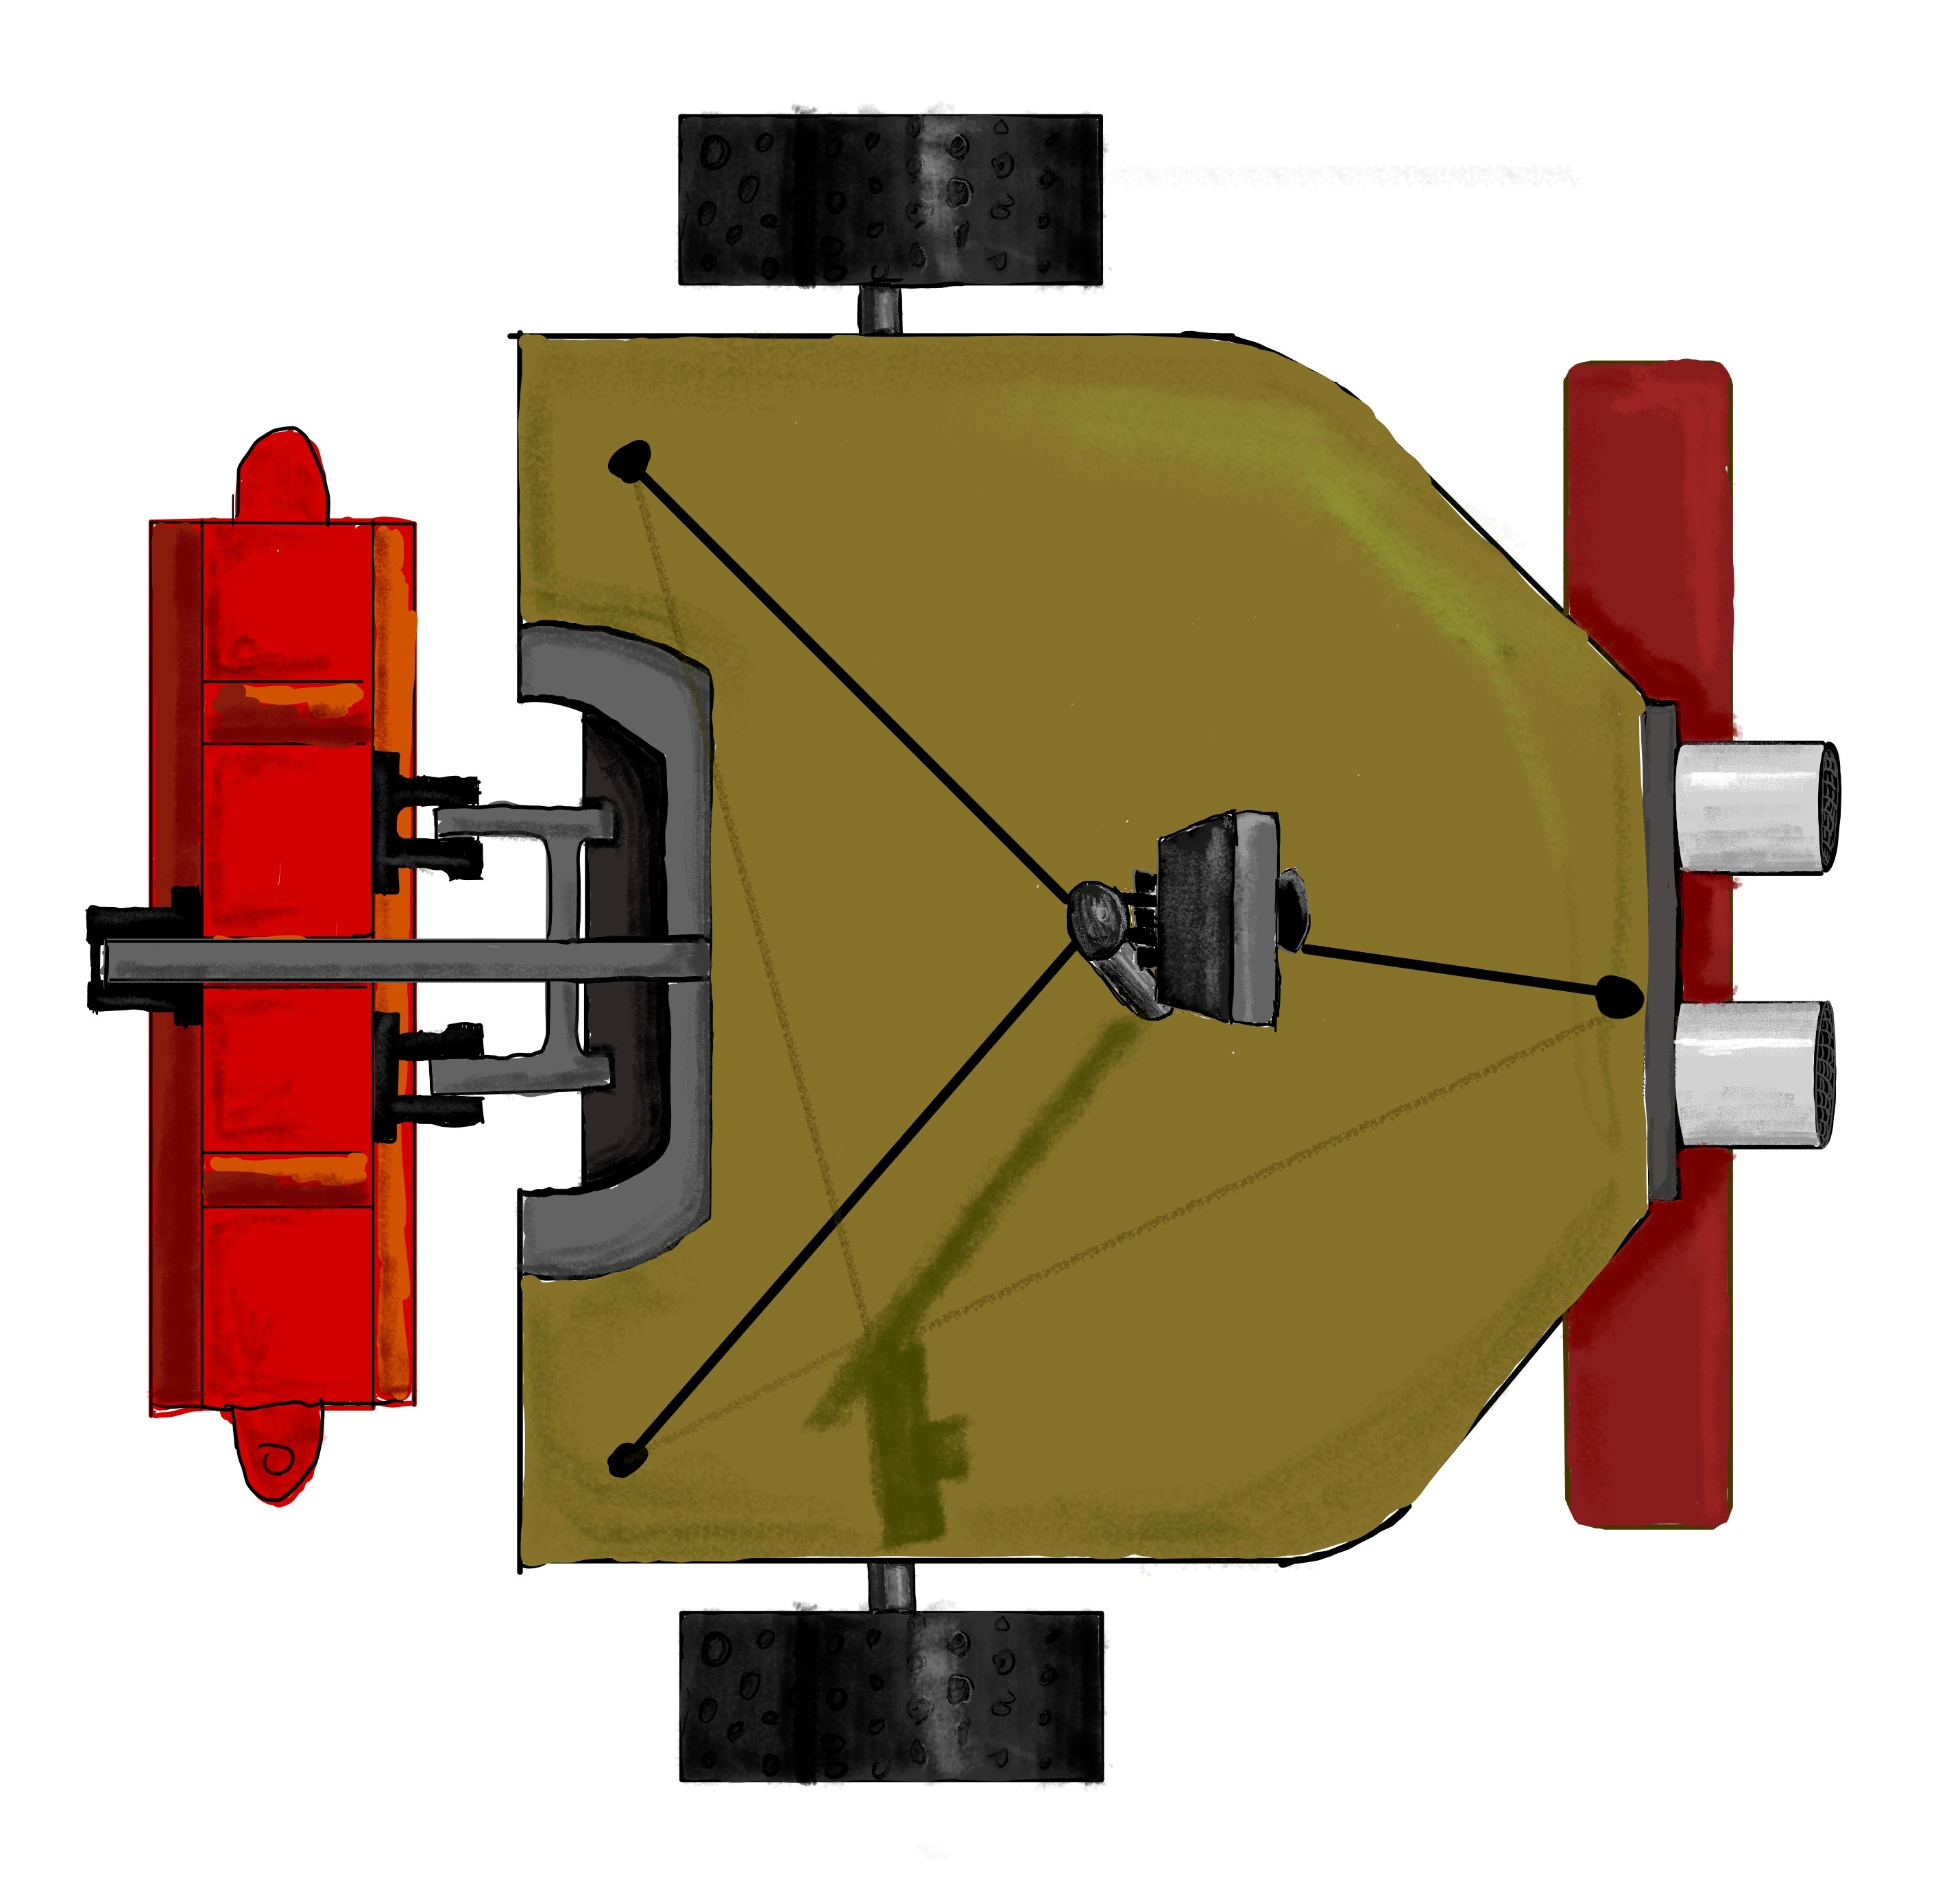
\includegraphics[width=0.5\textwidth]{assets/gesamtkonzept/Skizze-Fahrzeugkonzept.jpg}}


\author{
\begin{tabular}{ l l l}
  \textbf{Gruppe 4} && \\
  Kasper Jonah & jonah.kasper@stud.hslu.ch & Elektrotechnik\\
  Zimmermann Ivan & ivan.zimmermann@stud.hslu.ch & Elektrotechnik \\
  Schmid Lukas & lukas.schmid@stud.hslu.ch & Informatik\\
  Meyer Alina & alina.meyer@stud.hslu.ch & Informatik \\
  Mumenthaler Marc & marc.mumenthaler@stud.hslu.ch & Maschinentechnik\\
  von Atzigen Elias & elias.vonatzigen@stud.hslu.ch & Maschinentechnik \\
  \\
  \textbf{Betreuender Dozent} && \\
  Thalmann Markus & markus.thalmann@hslu.ch & Elektrotechnik \\
  \\
  \\
  \\
  TA.BA\_PREN1.H2401 &&\\
\end{tabular}
}
\date{\today}


    \maketitle
    \newpage

    \section*{Abstract}

Diese Arbeit präsentiert das Design eines Roboters, der autonom ein Wegentz durchqueren kann und dabei zufällig platzierte Hindernisse erkennt. Dazu wurden die Teilfunktionen der Roboters definiert und durch Prototyping entwickelt.

Es wurde ein Roboter designed, der den Linien auf einem Wegenetz folgen kann, sich darauf um die eigene Achse drehen kann und Hindernisse selbständig erkennt und einordnet. Bewegliche Hindernisse auf dem Wegenetz können sicher angehoben und wieder zurückgestellt werden.

\begin{figure}[H]
\centering
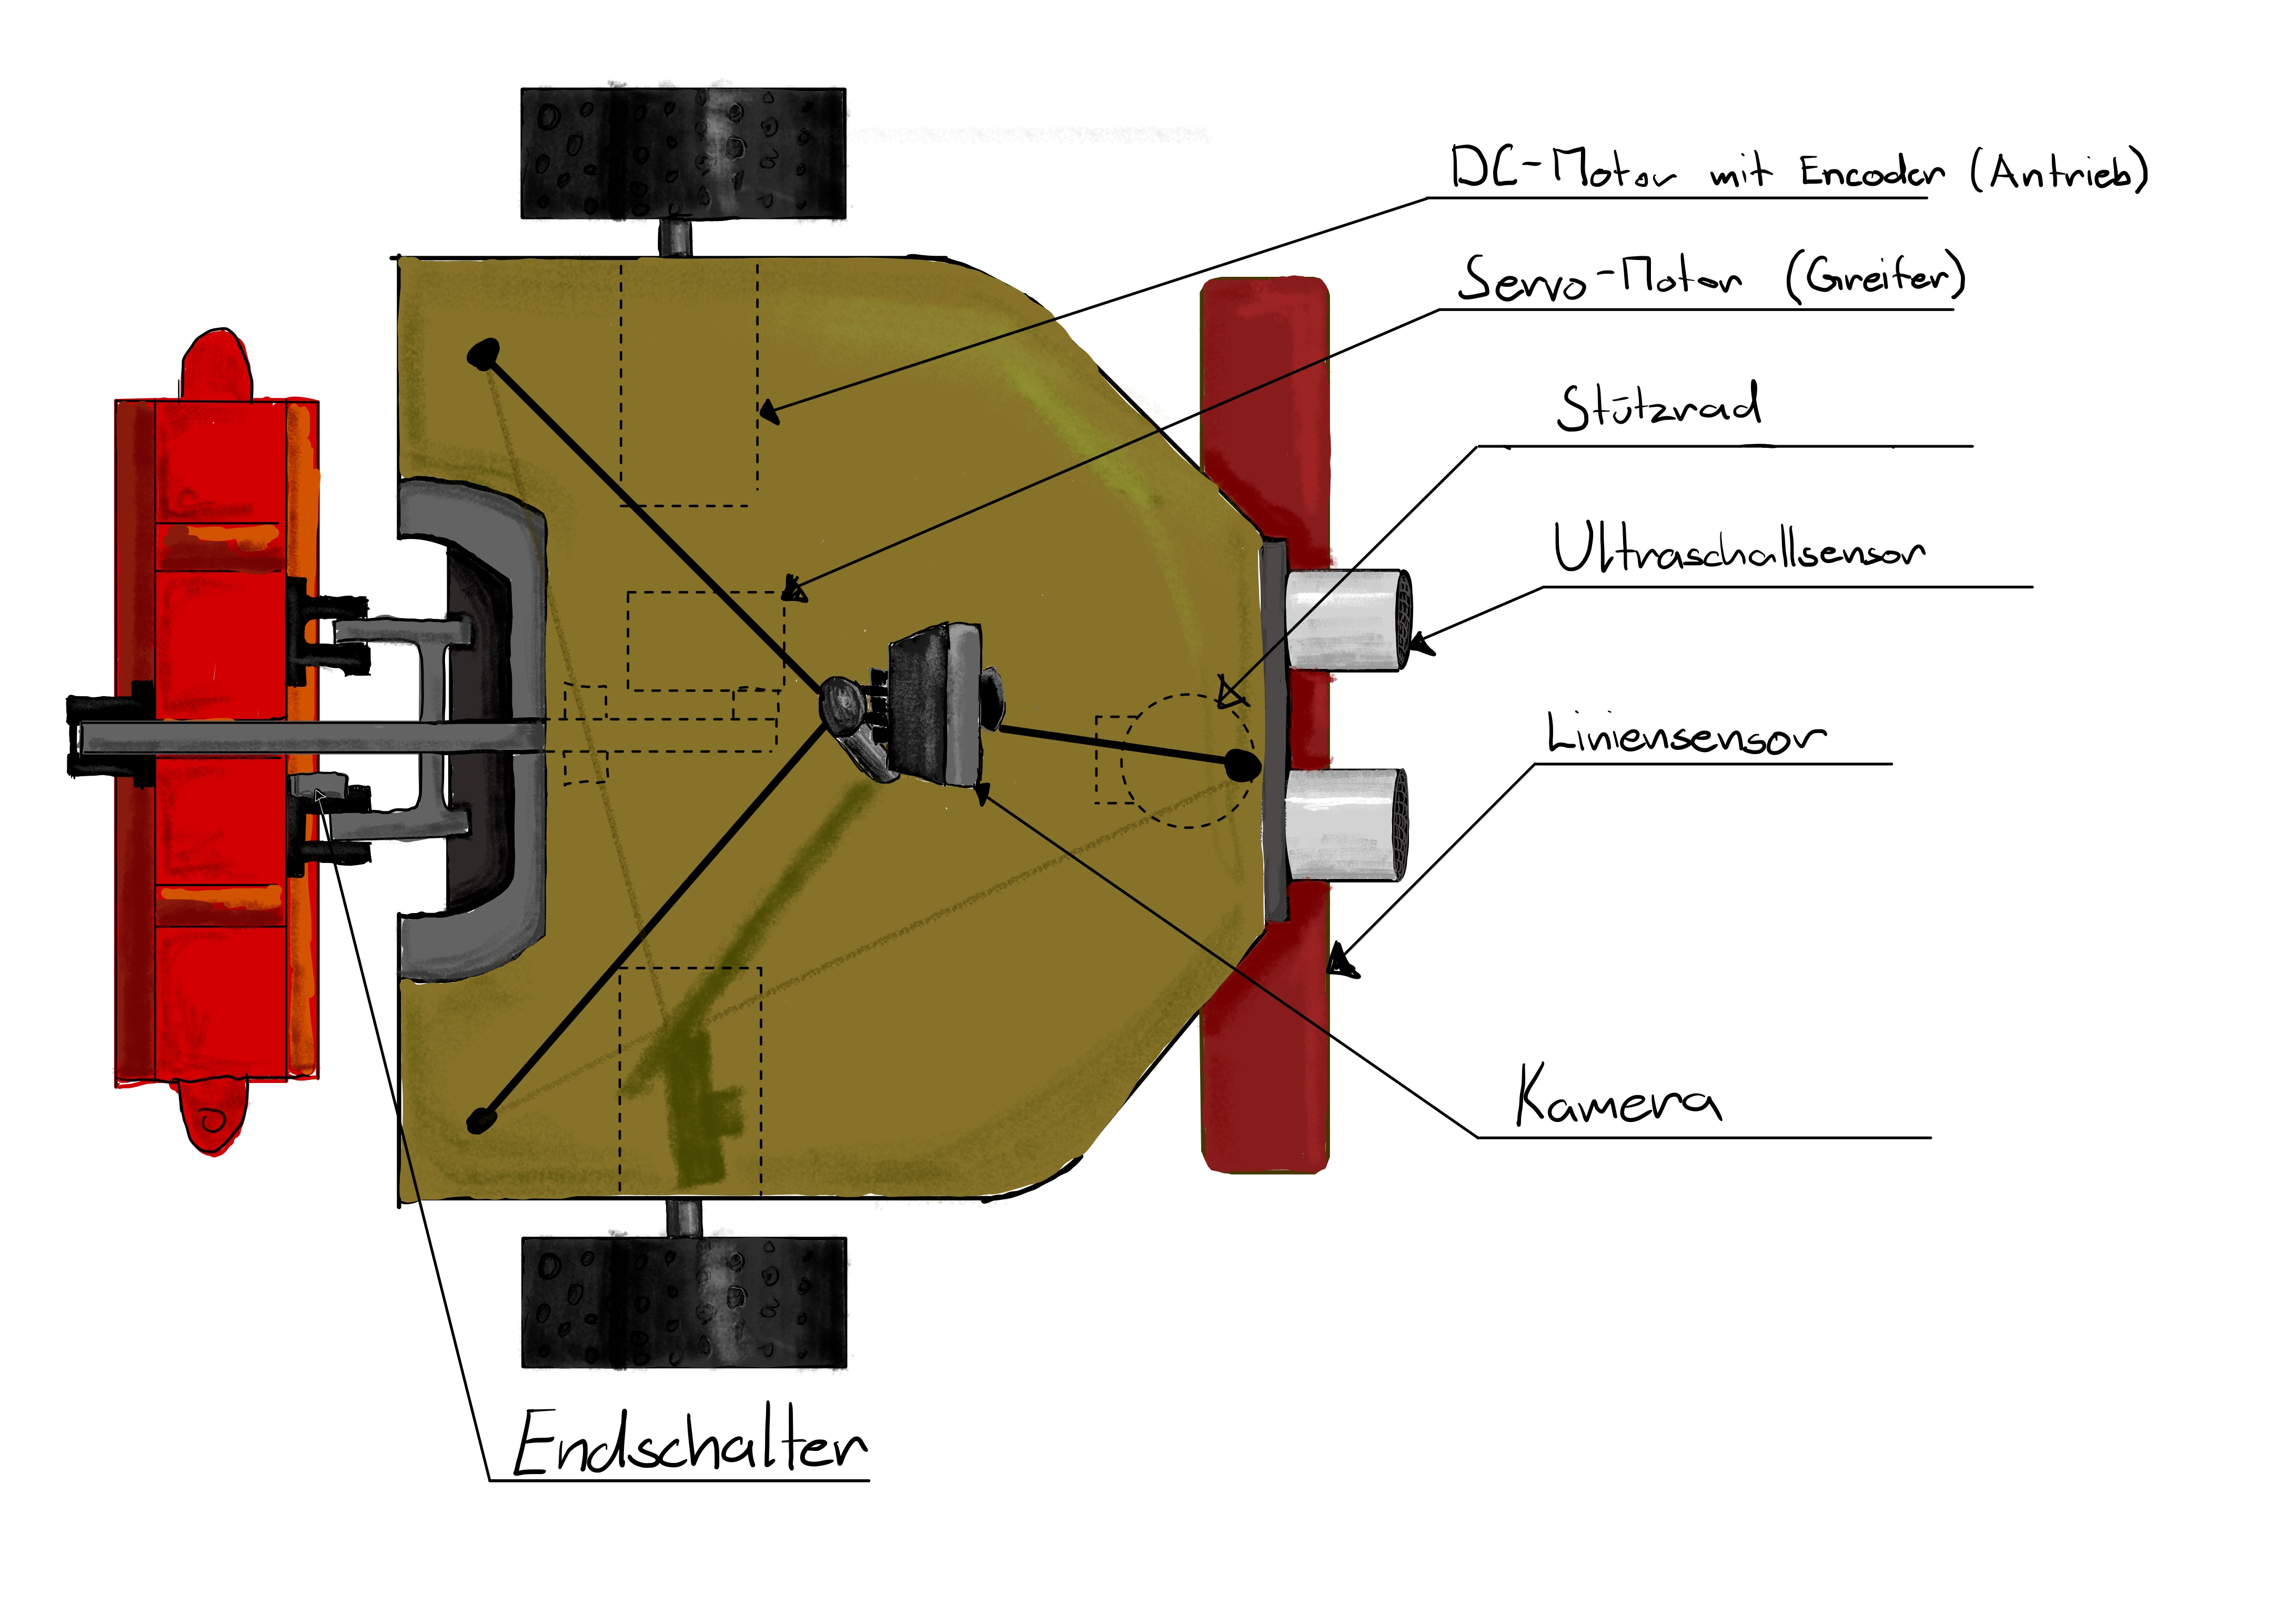
\includegraphics[width=0.7\textwidth]{assets/gesamtkonzept/Skizze-Fahrzeugkonzept-Beschriftet.jpg}
\caption{Konzeptskizze Gesamtkonzept}
\label{fig:robot_concept-scetch_labeld-abstract}
\end{figure}

Der Roboter wird das Wegenetz auf drei Rädern durchfahren, wobei zwei davon mit Motoren betrieben werden. Ein Liniensensor bestehend aus Fototransistoren wird eingesetzt, damit der Roboter die Linien des Wegenetzweks nicht verlässt.

Die Hebervorrichtung, die der Roboter braucht, um bewegliche Hindernisse zu beseitigen, wird mit einem Greifer mit flexiblen Backen umgesetzt. Ein Ultraschallsensor detektiert, sobald sich eine Barriere in der Nähe befindet, damit sich der Greifer langsam darauf zu bewegen kann. Sobald die Endschalter am Greifer betätigt werden, greift dieser zu. Durch die doppelte Hindernisdetektierung ist der Roboter zuverlässig und durch die Konstruktion des Greifers, kann das Hindernis sicher gefasst werden, auch falls sich dieses schräg auf der Linie befindet.

Hindernisse werden mit einer Kamera und Bilderkennung erkannt, damit der Roboter weiss, welche Wege befahrbar sind. Es kann Zeit eingespart werden, da die Hindernisse aus der Distanz detektiert werden.

Um die Machbarkeit zu simulieren wurde ein Simulator programmiert. Dieser stellt dar, wie der Roboter sich durch das Wegenetz fortbewegt und misst die Zeit. Zusätzlich dient er als Grundlage zur Navigation im richtigen Roboter.

Das finale Design des autonomen Roboters bietet eine effiziente und sichere Lösung, um das Wegenetz zu durchqueren. Es ist eine zuverlässige Grundlage für die Umsetzung in Produktentwicklung 2.



    \tableofcontents\thispagestyle{fancy}
    \newpage
    \listoffigures\thispagestyle{fancy}
    \newpage
    \listoftables
    \newpage
    \subfile{glossary.tex}

%%%%%%%%%%%%%%%%%%%%%%%%%%%%%%%%%%%%%%%%%%%%%%%%%%%%%%%%%%%%%%%%%%%%%%%%%%%%%%%%%%%%%%%%%%
%%%%%%%%%%%%%%%%%%%%%%%%%% Add your file here %%%%%%%%%%%%%%%%%%%%%%%%%%%%%%%%%%%%%%%%%%%%
%%%%%%%%%%%%%%%%%%%%%%%%%%%%%%%%%%%%%%%%%%%%%%%%%%%%%%%%%%%%%%%%%%%%%%%%%%%%%%%%%%%%%%%%%%

    % Include files
    \section{Einleitung}

In dieser Dokumenation wird im Rahmen von \acrfull{pren1} die Entwicklung eines autonomen Roboters geplant. Dieser Roboter soll in der Lage sein, ein Wegenetzwerk zu erkennen und diesem zu folgen. Auf den einzelnen Wegen können sich Hindernisse befinden. Die eine Art der Hindernisse sind Pillonen. Wenn sich diese auf einem Pfad befinden, kann dieser nicht befahren werden. Die andere Art der Hindernisse können entfernt werden. Damit der Pfad befahrbar ist, müssen diese jedoch wieder an der selben Stelle zurückgestellt werden.
Das Projekt wird in einem interdiszipilinären Team durchgeführt. Das Team besteht aus Studenten aus den Studiengängen Maschinentechnik, Elektrotechnik und Informatik. Dadurch sind die Kompetenzen, die benötigt werden für die Planung und die Umsetzung des Projektes vorhanden.

In diesem Bericht werden sowohl die Vorgehensweise, als auch die gesamte Planung des Projektes beschrieben. In der Planung wird beschrieben wie das geplante Gesamkonzept erarbeitet wurde. Als erstes wurde eine Technologierecherche durchgeführt. Die einzelnen Lösungen wurden evaluiert und kombiniert. Folgend wurden die Lösungskombinationen evaluiert, woraus sich das Konzept ergab.

Diese Planung bildet die Vorbereitung fuer \acrfull{pren2}. In \acrshort{pren2} wird der geplante Roboter entwickelt. Das Modul wird mit einem Wettbewerb abgeschlossen, wobei die einzelne Gruppen ihre Roboter gegeneinander antreten lassen.

Bei der Konzeptentwicklung des Roboters war es das Ziel einen möglichst simplen Roboter zu bauen, der funktioniert. Der Fokus liegt nicht darauf den schnellsten Roboter zu haben, er sollte jedoch effizient sein.
    \subsection{Aufgabenstellung}

Die Aufgabenstellung ist auf folgender Grafik skizziert. Zentral sind die variablen Bedingungen im Wegenetz. Die Strecke kann durch Pylonen gesperrte Knoten haben. Linien können komplett entfernt sein.  Auf einer Verbindungslinie kann sich ein Hindernis befinden, welches vom Roboter angehoben werden darf. Der Roboter muss danach das Hindernis an die ursprüngliche Stelle zurückstellen. Erreicht der Roboter das Ziel, muss es dies signalisieren.

\begin{figure}[H]
\centering
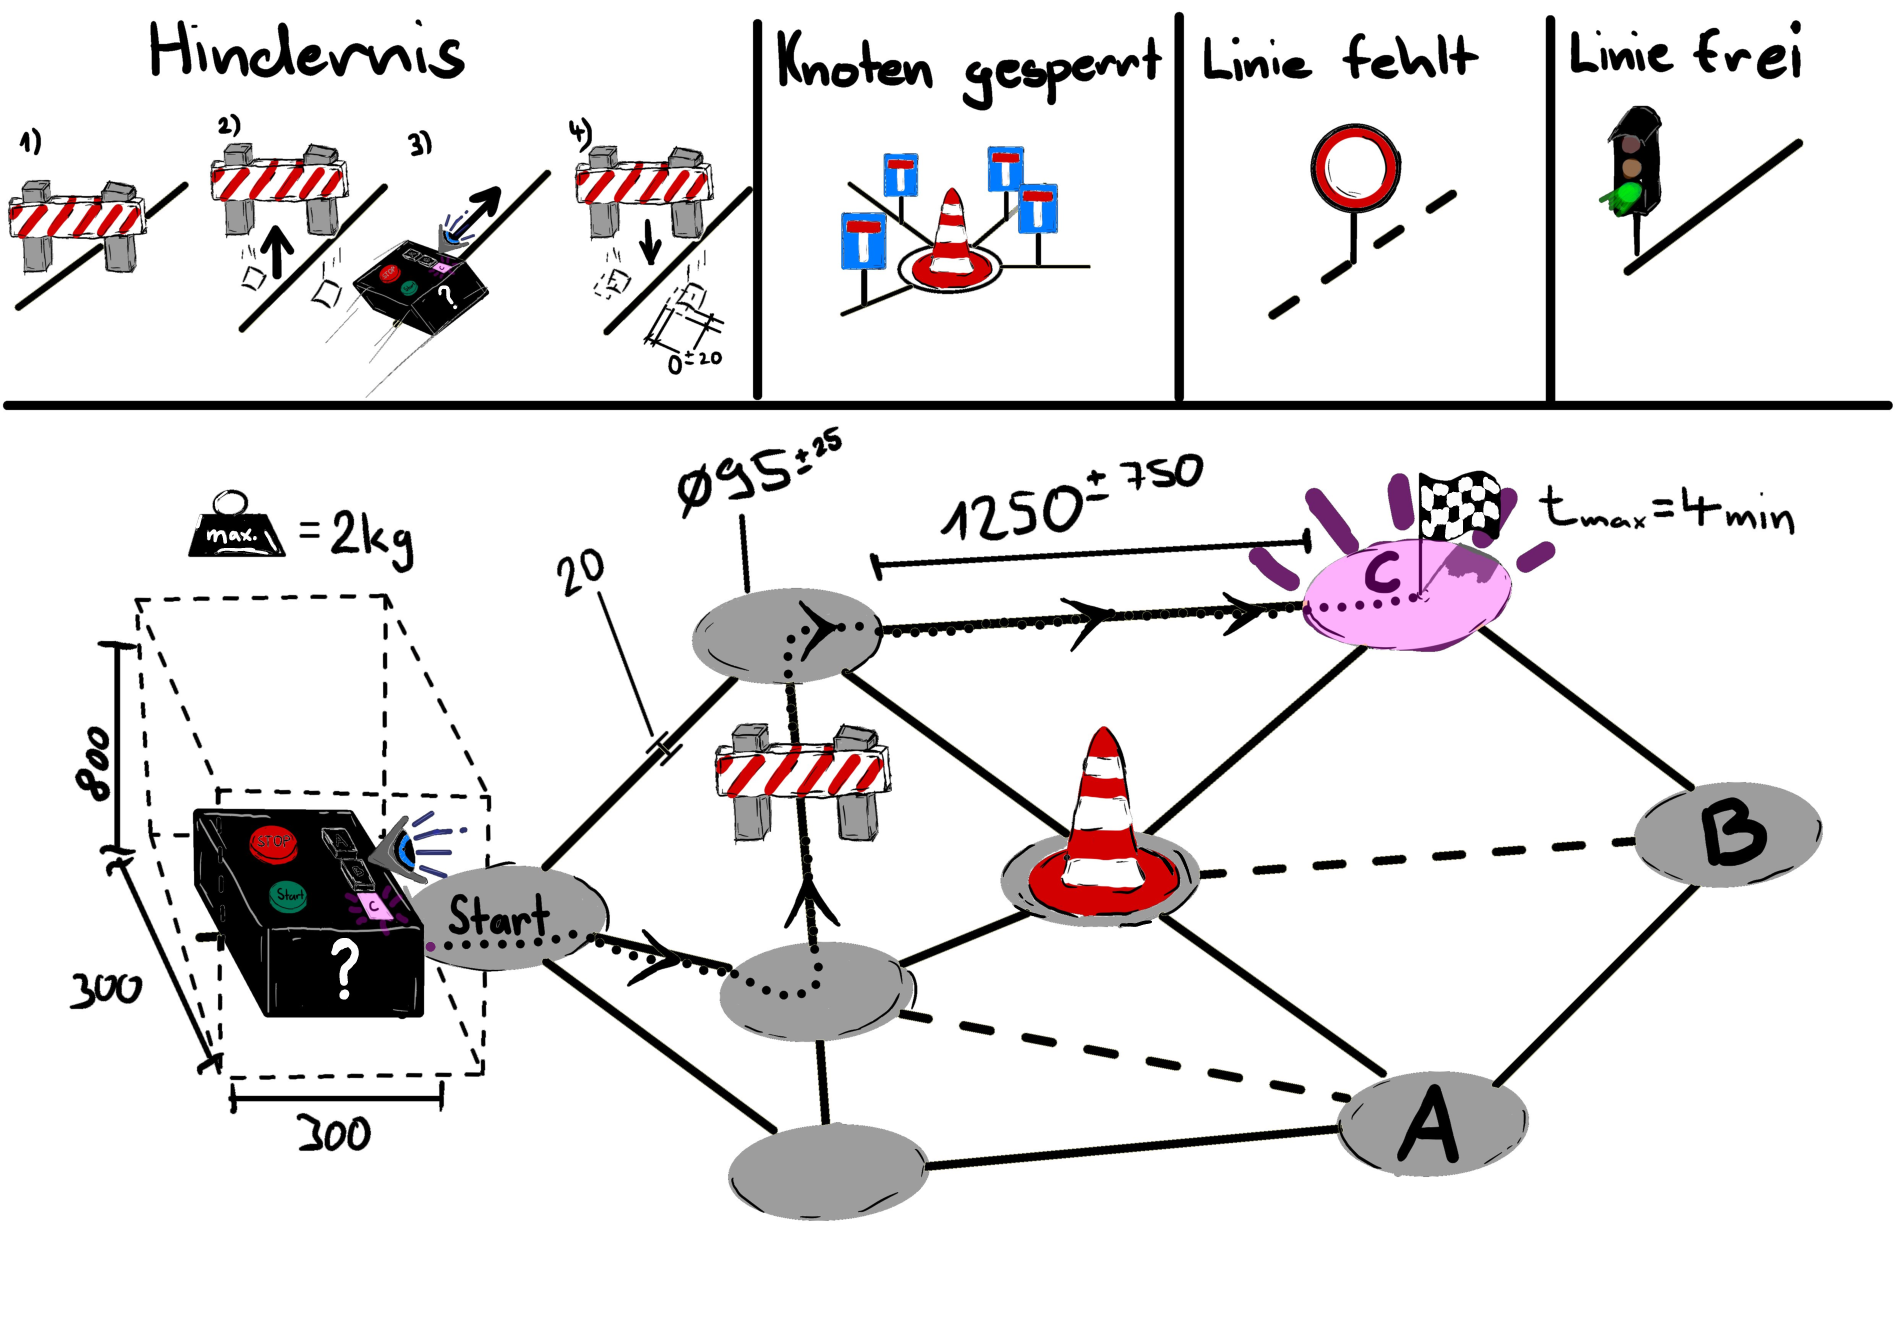
\includegraphics[width=\textwidth]{img/Skizze_Aufgabenstellung_v4.2.png}
\caption{Aufgabenstellung}
\label{fig:aufgebanstellung}
\end{figure}

\subsection{Anforderungsliste}

Die Anforderungsliste wurde basierend auf der Aufgabenstellung erstellt und anschliessend von dem betreuenden Dozenten freigegeben. Zur Strukturierung wurden die Anforderungen in sieben Gruppen gegliedert: Gerät, Sicherheit, Software, Nachhaltigkeit, Demonstration, Wegenetz und Budget. Die einzelnen Anforderungen wurden in die Kategorien Fest-, Mindest-- und Wunschanforderungen unterteilt. Zu jeder Anforderung wurde mindestens eine Fachrichtung definiert, welche für die Einhaltung der
Anforderung verantwortlich ist.

Die vollständige Anforderungsliste befindet sich im Anhang im Kapitel \nameref{anforderungliste}.

    \section{Gesamtkonzept}

In den folgenden Kapiteln wird das erarbeitete Konzept des Roboters vorgestellt. Dafür wird zuerst eine Skizze gezeigt, die den geplanten Roboter visualisiert, danach werden die Komponenten und Technologien, die im Roboter verwendet werden, aufgelistet. Nachfolgend werden die einzelnen Teilfunktionen, die der Roboter während einem Durchlauf benötigt erläutert. 

Das Konzept wurde mithilfe des Prototypings getestet. Dies ist im Anhang in Kapitel \nameref{prototyping} zu finden.

\subsection{Visualisierung}

Die Einzelteile des Roboters sollen wie auf Abbildung \ref{fig:robot_concept-scetch_labeld} gezeigt zusammengesetzt werden.

\begin{figure}[H]
\centering
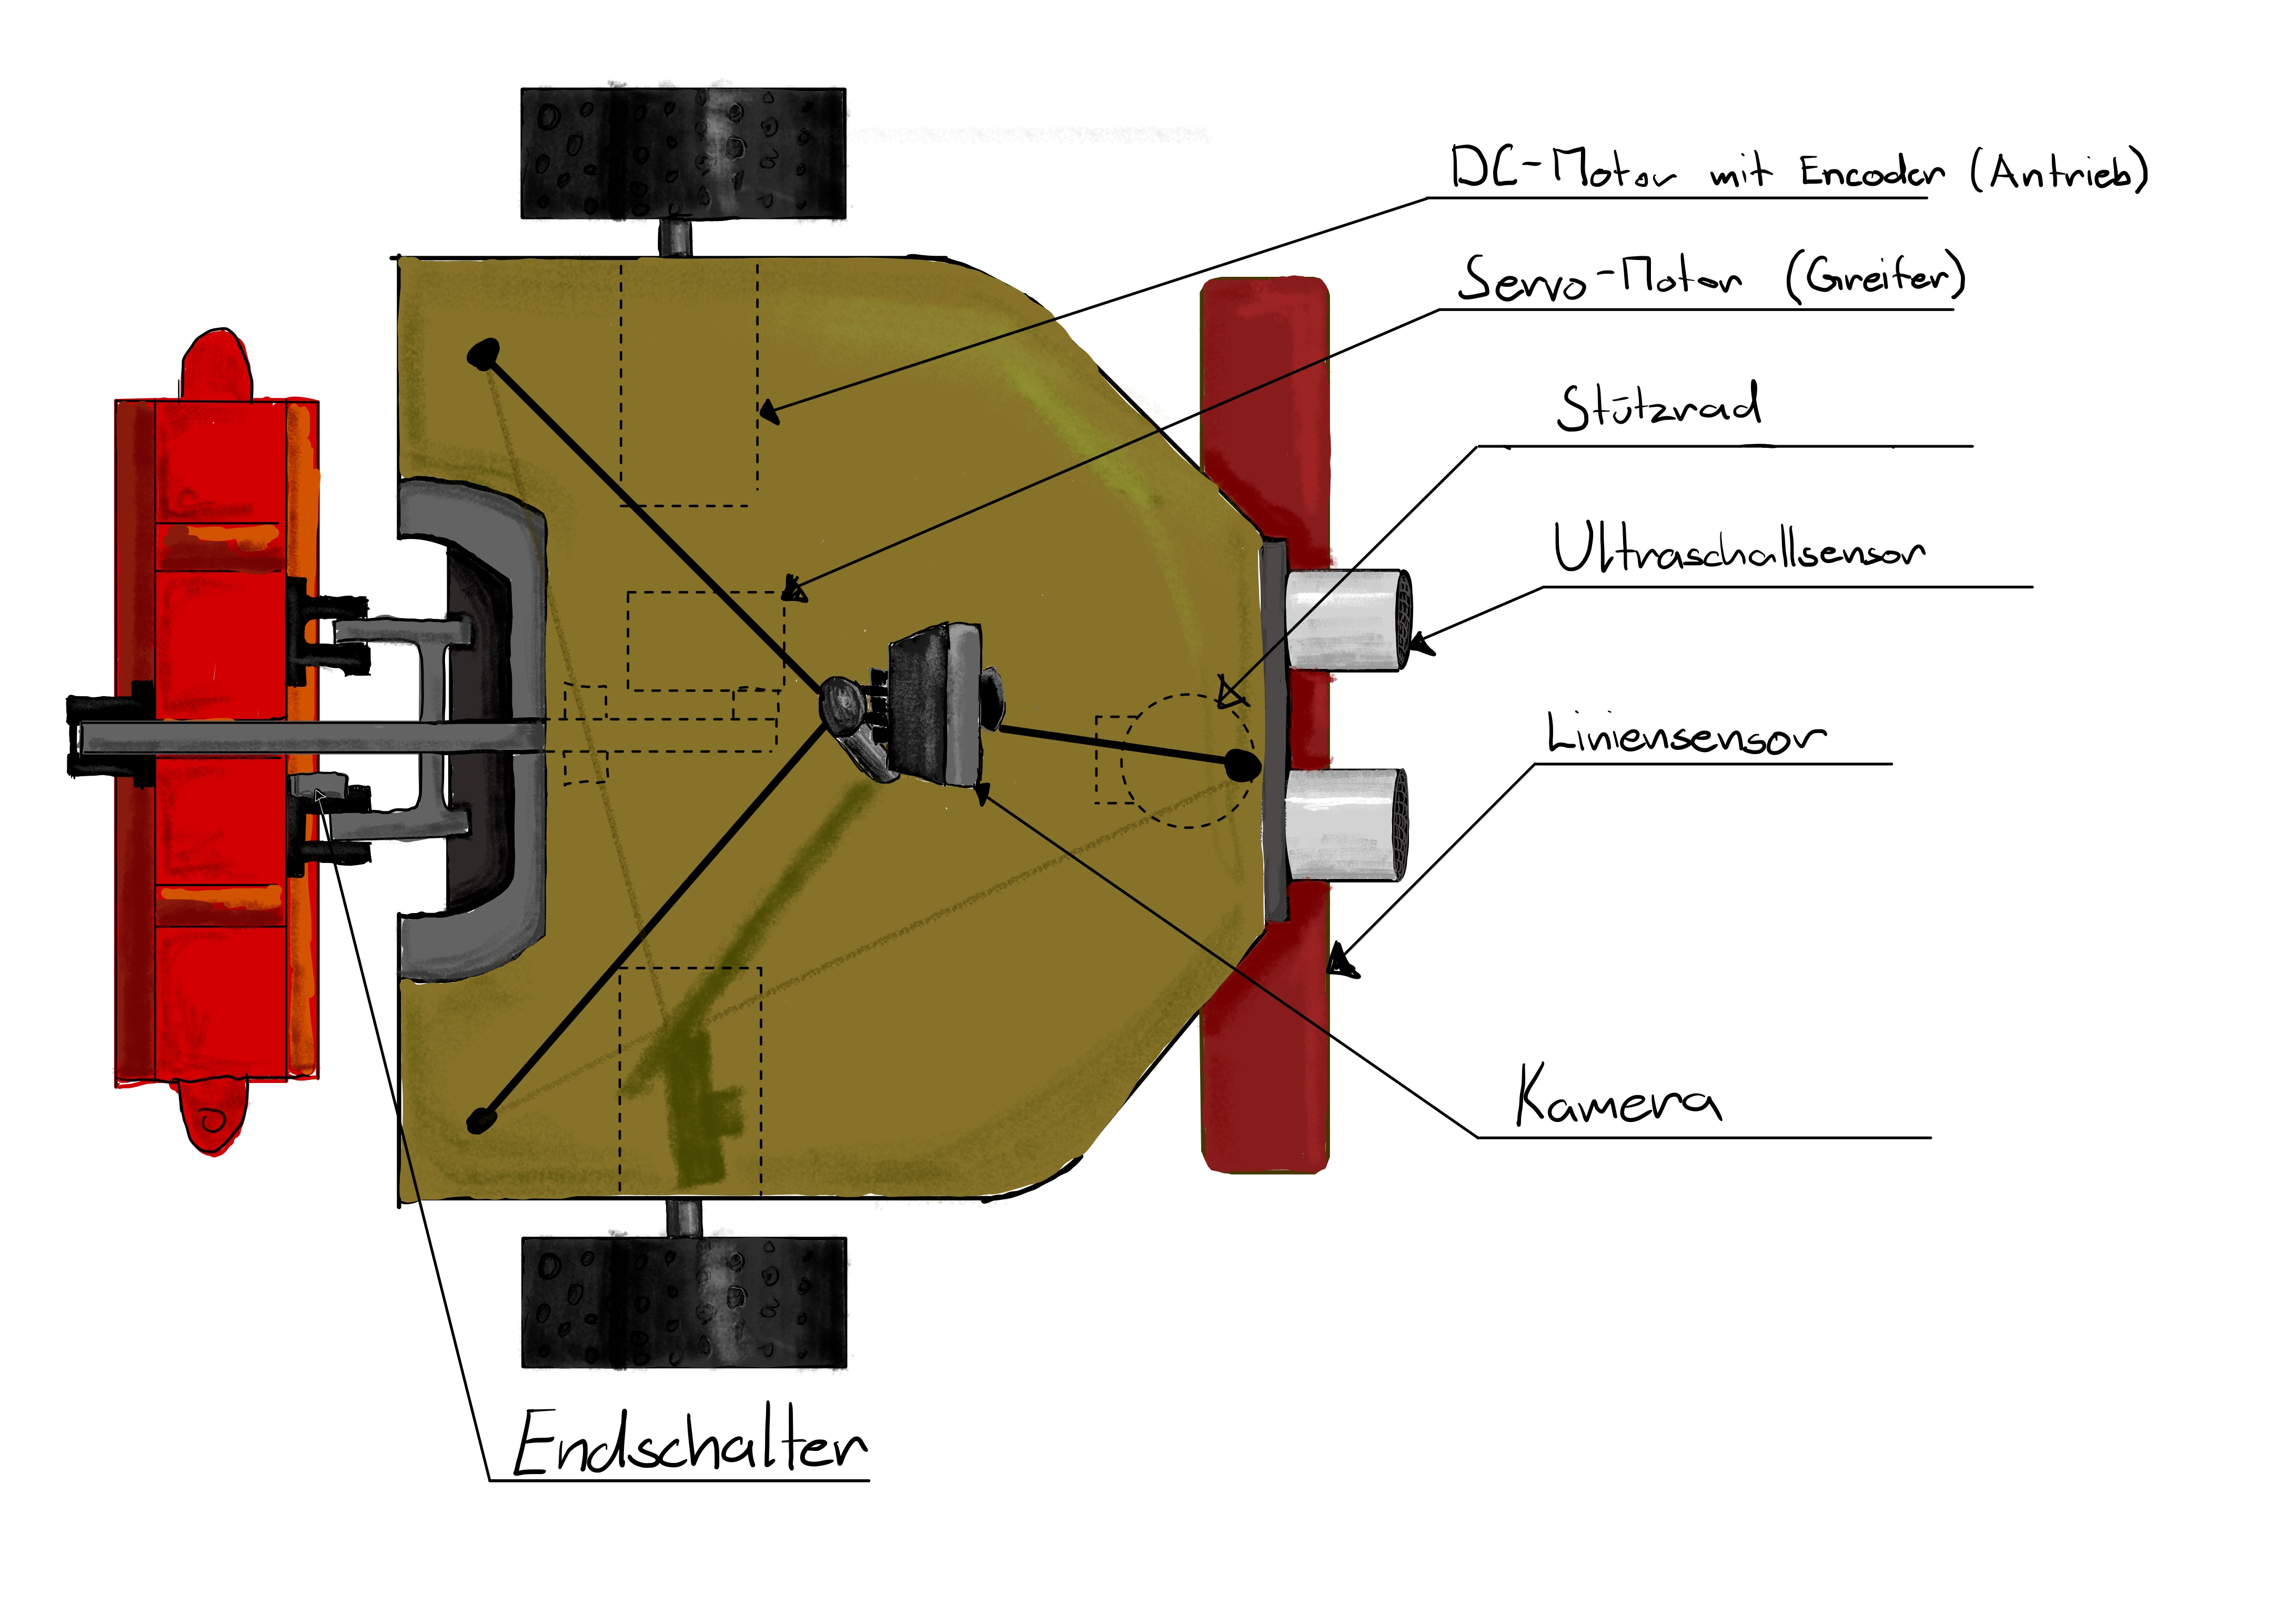
\includegraphics[width=\textwidth]{assets/gesamtkonzept/Skizze-Fahrzeugkonzept-Beschriftet.jpg}
\caption{Konzeptskizze Gesamtkonzept}
\label{fig:robot_concept-scetch_labeld}
\end{figure}

\subsection{Komponenten}
Für das Konzept wurden die auf Abbildung \ref{table:mk-all} ersichtlichen Komponenten mithilfe der Technologierecherche (siehe Anhang \nameref{techrecherche}) und anschliessenden morphologische Kästen (siehe Anhang \nameref{mk}) und Nutzwertanalysen (siehe Anhang \nameref{nutzwertanalyse}) ermittelt. 

\begin{table}[H]
\centering
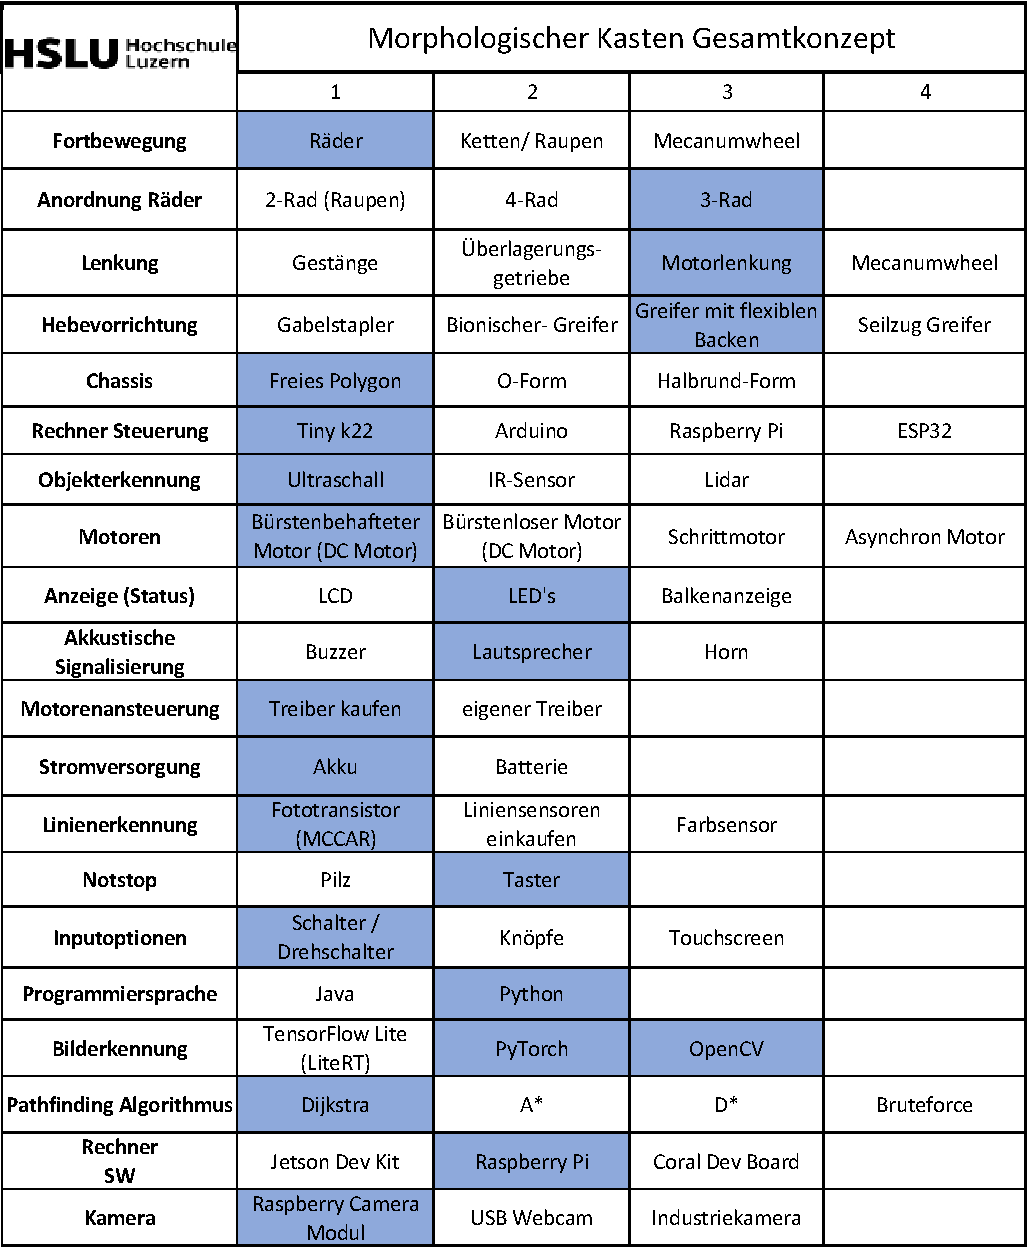
\includegraphics[width=\textwidth -20mm]{assets/MK-all.pdf}
\caption{Morphologischer Kasten: Gesamtkonzept}
\label{table:mk-all}
\end{table}

Es ist geplant einen Roboter in Form eines freien Polygons zu bauen, der sich mit drei Rädern fortbewegt und eine Motorlenkung besitzt. Hindernisse kann der Roboter dank einem Greifer mit flexiblen Backen anheben. Dies ist in der vorherigen Abbildung \ref{fig:robot_concept-scetch_labeld} ersichtlich.

Die Steuerung wird auf einem \gls{tinyk22} betrieben. Die Distanz zu den Objekten wird mittels einem Ultraschallsensor erkannt. Die bürstenbehafteten Motoren werden mit einem gekauften Treiber angesteuert. Die Stromversorgung läuft über einen Akku. Der Akkustand und der Status des Roboters werden durch \acrfull{led} angezeigt. Damit der Roboter die Linien erkennt, wird ein Liniensensor mit Phototransistoren verwendet. Das Ziel wird über einen Drehschalter vom Benutzer ausgewählt.
Wenn der Roboter das Ziel erreicht, verkündet er dies über einen Lautsprecher. Im Notfall wird der Roboter über einen Taster ausgeschaltet.

Die Bildverarbeitung und Navigation werden in Python programmiert und laufen auf einem Raspberry Pi. Zur Bilderkennung wird eine Kombination von \gls{pytorch} und \gls{opencv} verwendet. Die Bilder werden mit einer Raspberry Pi Camera aufgenommen. Der kürzeste Weg zum Ziel wird mit einem \gls{dijkstra} Algorithmus berechnet.

\subsection{Ablauf}

Der Ablauf einer Durchfahrt ist im Ablaufdiagramm \ref{fig:ablaufdiagramm} aufgezeigt.
Die Schritte, die mit einem Plus markiert sind, sind in den folgenden Kapiteln als Subprozesse detailliert definiert.

Um den Graph zu traversieren, wird eine iterative Herangehensweise umgesetzt. Durch die Spiegelung des Bodens, die Grösse des Graphes und die Einschränkung der Höhe des Roboters, ist es nicht möglich, am Start ein Bild des gesamten Graphens zu machen und dabei die Hindernisse und die fehlenden Linien zu erkennen. Deshalb werden iterativ bei jedem Knoten die ausgehenden Linien geprüft.

\begin{figure}[H]
\centering
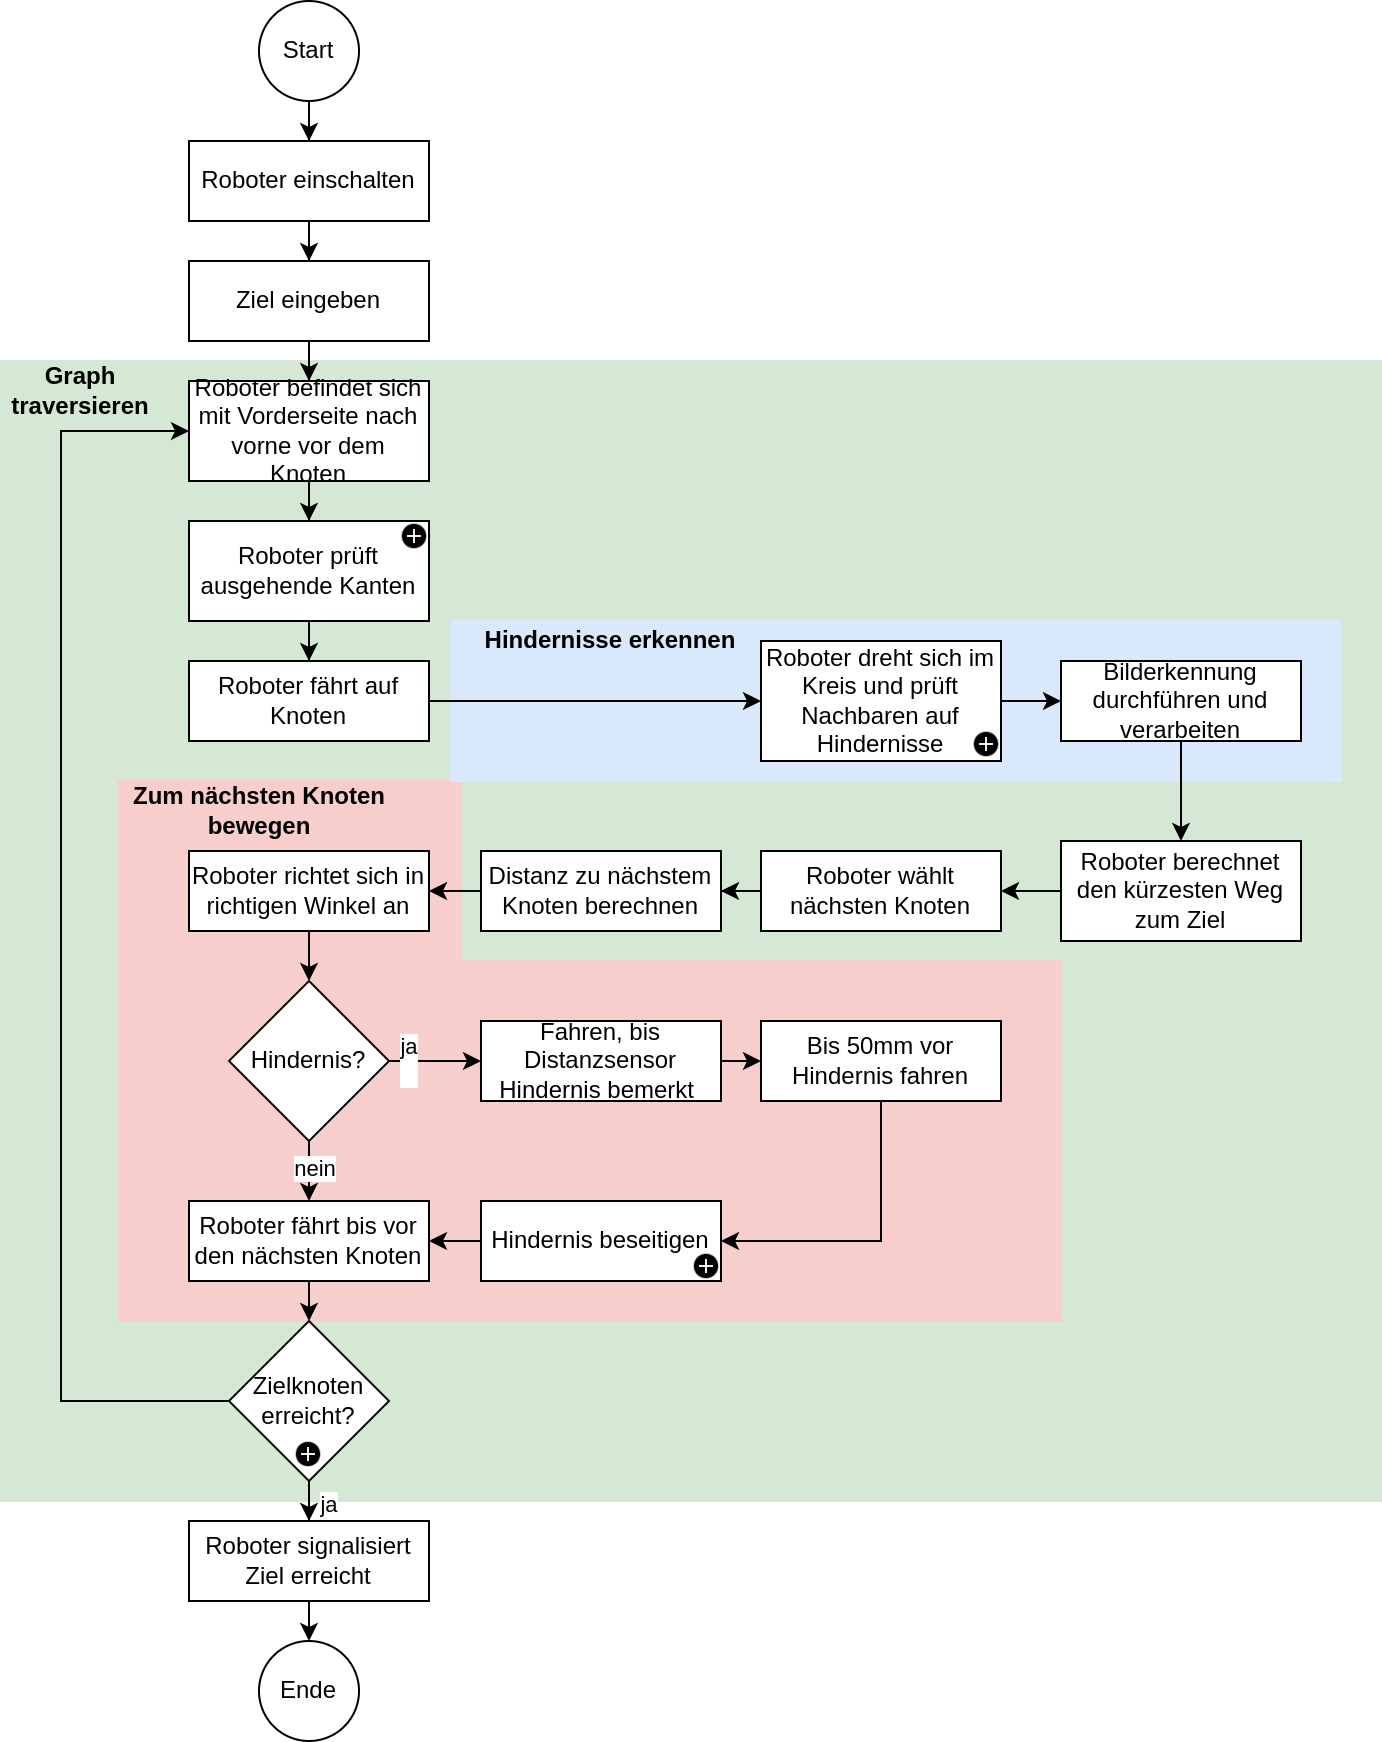
\includegraphics[width=\textwidth]{assets/gesamtkonzept/ablaufdiagramm.png}
\caption{Ablaufdiagramm}
\label{fig:ablaufdiagramm}
\end{figure}

\subsubsection{Ausgehende Kanten erkennen}\label{outgoing-angles}

Um alle ausgehenden Kanten und deren Winkel zu erkennen, wird der folgende Ablauf in Abbildung \ref{fig:ablaufdiagramm-kanten-erkennen} durchlaufen. Dies ist nötig, damit der Roboter weiss, in welche Richtung er sich drehen muss, um auf die nächste Kante zu gelangen. Ebenfalls können so fehlende Linien erkannt werden.

Falls es weniger Kanten gibt als erwartet, werden die erhaltenen Winkel zu den einzelnen möglichen Bereichen zugeordnet. In dem Bereich, in welchem kein Winkel zugeordnet wurde, fehlt eine Linie. Folglich aktualisiert der Roboter seine internen Informationen: Eine Linie wird aus dem Grundgraphen entfernt und die Basiswerte der Winkel werden mit den gemessenen Werten ersetzt.

Nachdem der Roboter den nächsten Knoten berechnet hat, wird der Winkel zur richtigen ausgehenden Kante an die Steuerung gesendet. Der Roboter dreht sich, um auf dieser Linie weiterzufahren.

\begin{figure}[H]
\centering
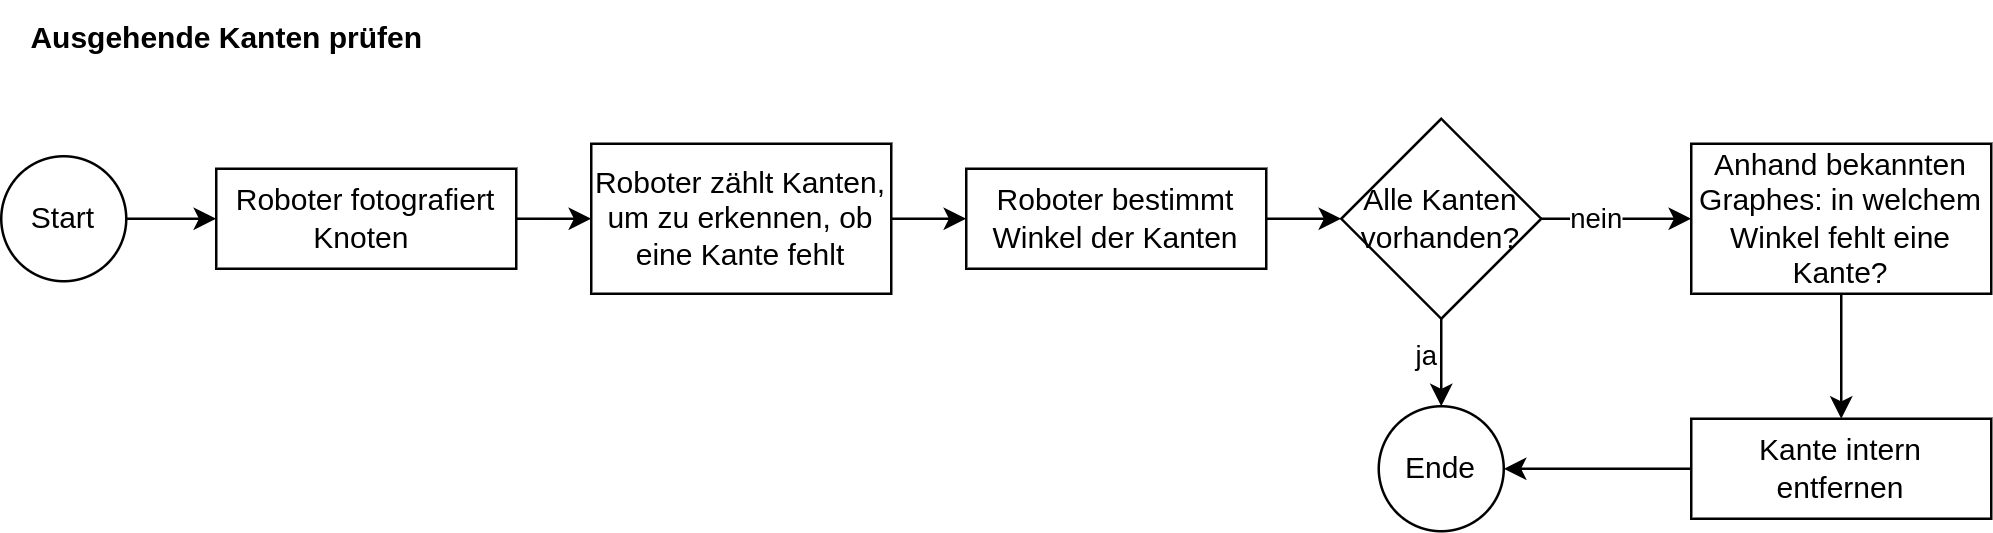
\includegraphics[width=\textwidth]{assets/gesamtkonzept/ablaufdiagramm-kanten-erkennen.png}
\caption{Ablaufdiagramm ausgehende Kanten erkennen}
\label{fig:ablaufdiagramm-kanten-erkennen}
\end{figure}

\textbf{Ablauf detailliert erklärt}

Der Roboter bewegt sich auf einen Knoten zu und hält 15 cm vor diesem an. Der Knoten wird fotografiert und der Roboter fährt anschliessend auf den Knoten. Das Bild wird mit \gls{opencv} zuerst so entzerrt, dass der Knoten gerade von oben dargestellt wird. Danach werden die einzelnen Winkel gemessen. Dies ist im Prototyping Kapitel im Anhang \nameref{winkelerkennung} ausführlicher beschrieben. Das Resultat dieser Objekterkennung ist eine Liste mit Winkeln. Im Fall, der auf Abbildung \ref{fig:angle-recognition} gezeigt ist, würde die Liste \verb|[3, 41, 68, 127]| erstellt werden.

\begin{figure}[H]
\centering
\begin{subfigure}{0.45\textwidth}
\centering
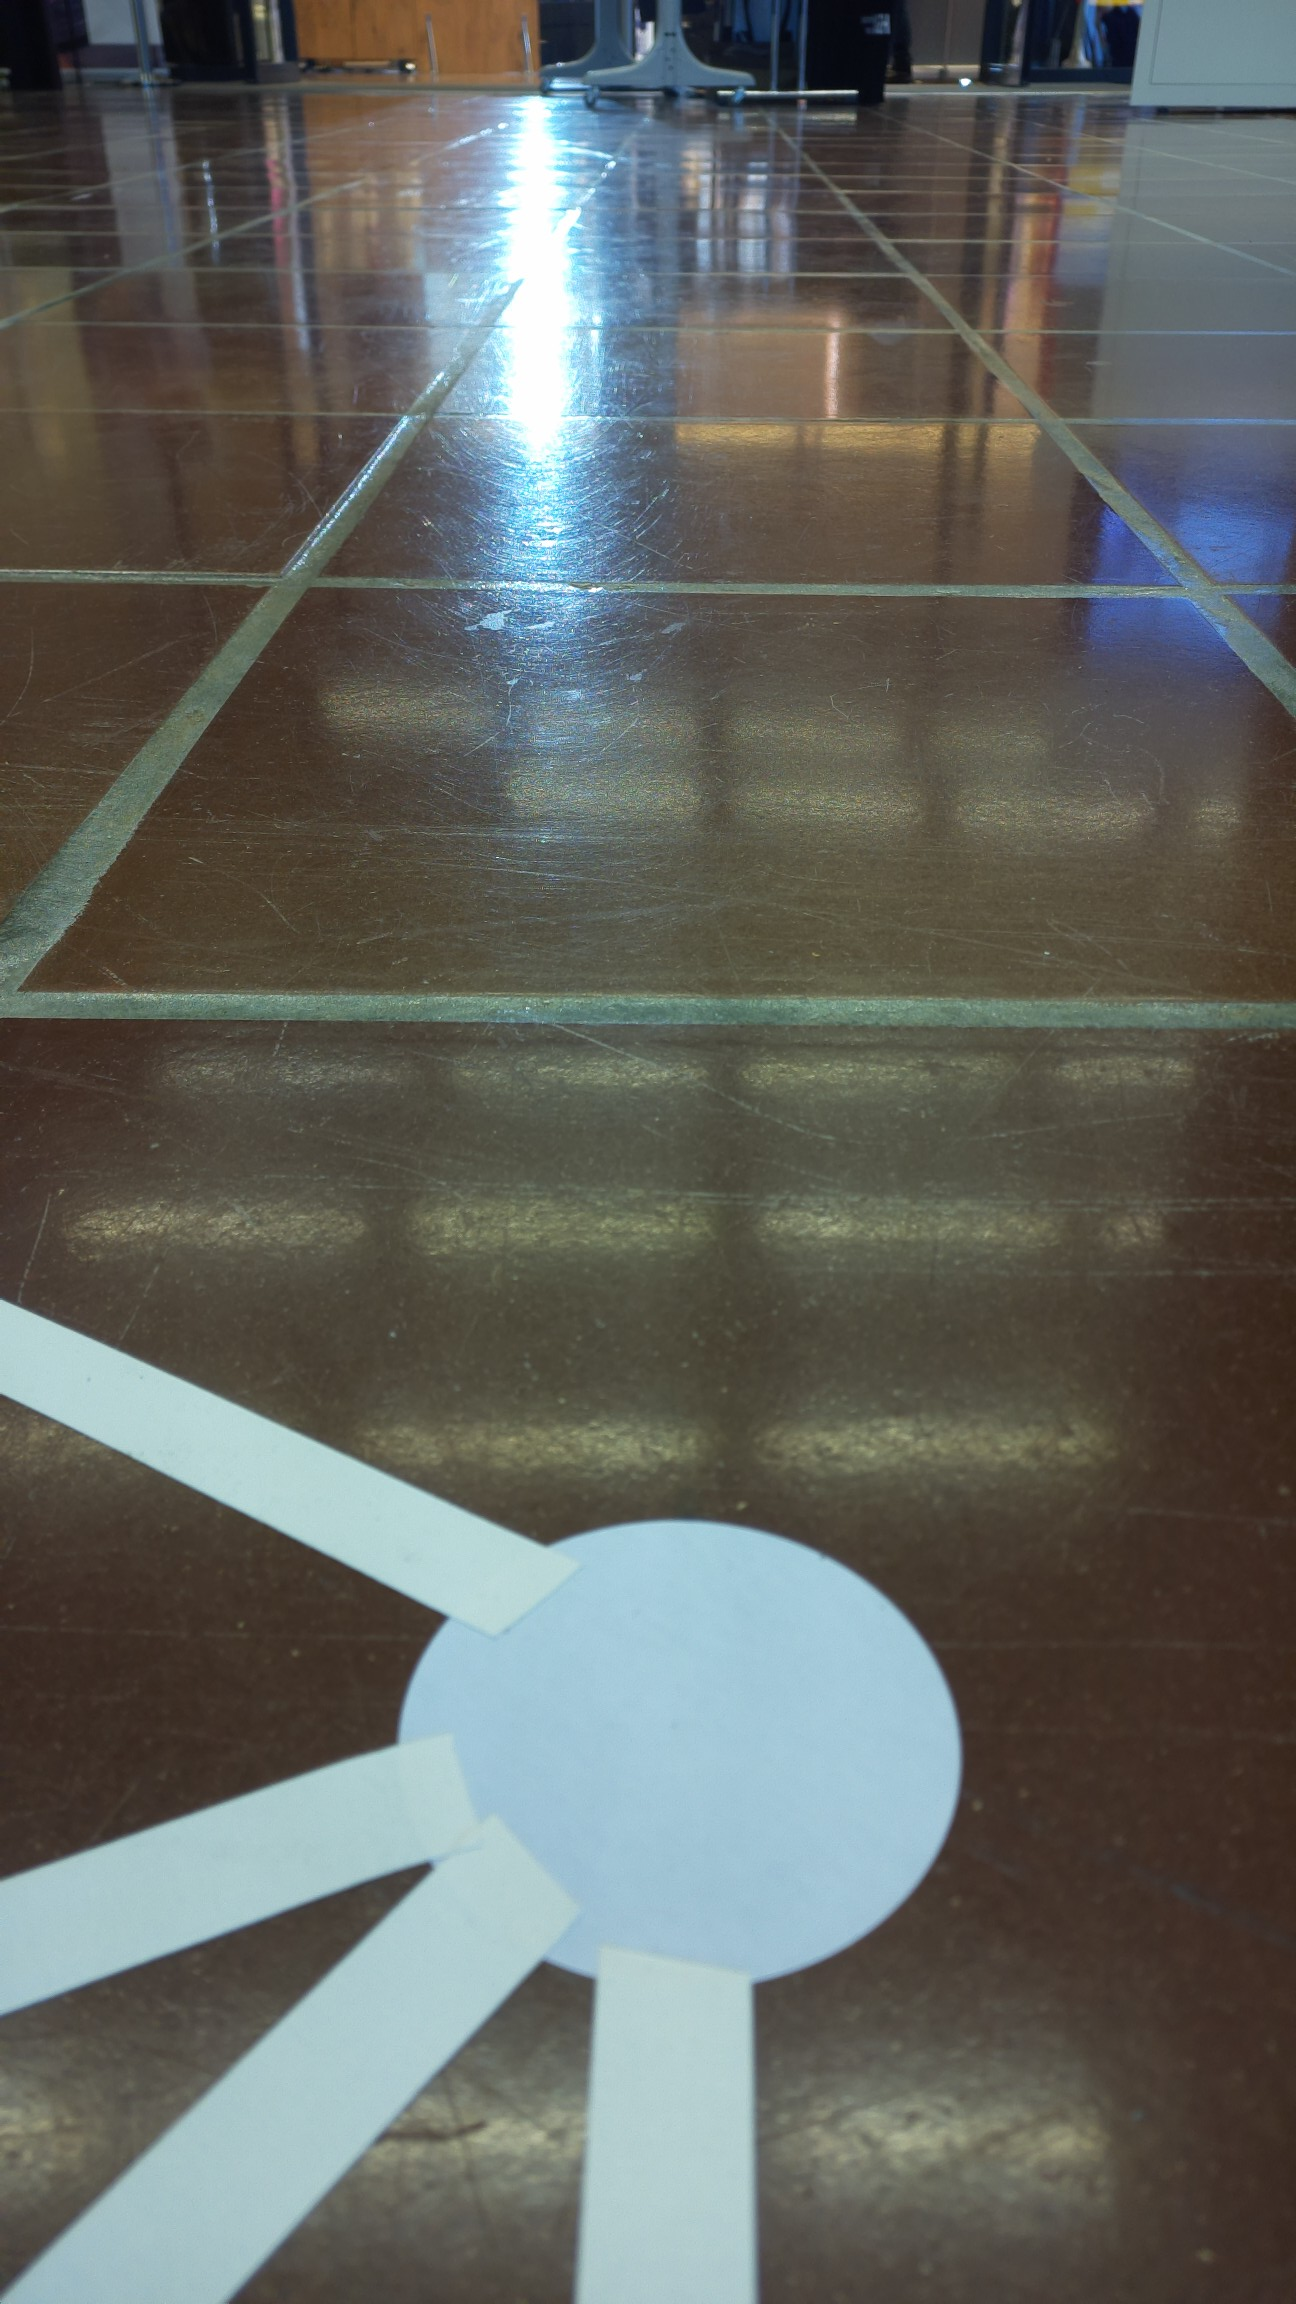
\includegraphics[width=0.95\linewidth]{assets/informatik-prototyp/opencv/angle_detection/image_taken_by_pi_camer_before_node.jpg} 
\caption{Knoten mit 15cm Abstand}
\label{fig:node-15cm-before}
\end{subfigure}
\begin{subfigure}{0.45\textwidth}
\centering
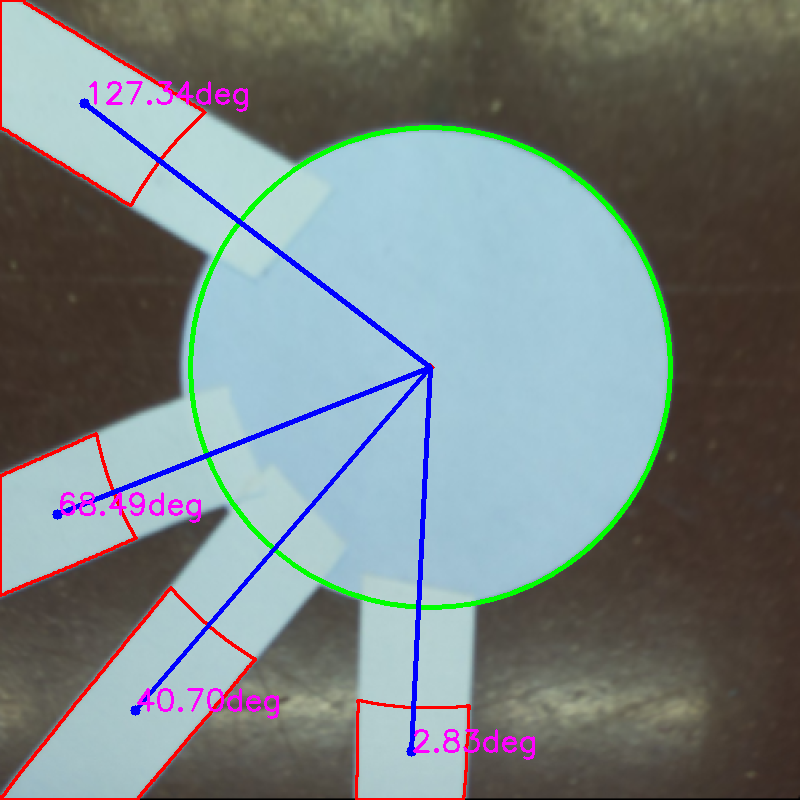
\includegraphics[width=0.95\linewidth]{assets/informatik-prototyp/opencv/angle_detection/node_with_edge_angles_annotated.png} 
\caption{Knoten mit gemessenen Winkeln}
\label{fig:node-angles}
\end{subfigure}

\caption{Winkelerkennung}
\label{fig:angle-recognition}
\end{figure}

Die erhaltene Liste mit Winkeln wird nun verwendet, um mögliche fehlende Linien zu erkennen und die Winkel intern zu speichern. Die internen Winkel werden verwendet, um den Roboter richtig auszurichten, wenn dieser auf die nächste Linie fährt.

Der Roboter selber hat einen Grundgraphen mit Winkeln gespeichert. Diese Winkel ergeben sich aus dem zur Verfügung gestellten Graph. Dabei werden die Winkel der Kanten im Graphen im Uhrzeigersinn gelesen. Dabei ist eine Linie, die nach 12 Uhr ausgeht, 0\textdegree, eine Linie nach 3 Uhr ist 90\textdegree, 6 Uhr ist 180\textdegree und 9 Uhr ist 270\textdegree. Der Roboter merkt sich, in welche Richtung er gerade schaut. Damit ergibt sich ein Offset, der verwendet wird, um die Winkel, die wie eine Uhr gelesen wurden, zu übersetzen. Mit dieser Information kann sich der Roboter dann richtig ausrichten.

Die Abbildung \ref{fig:angle-graphs-internal} soll visualisieren, wie die Winkel von jedem Knoten intern gespeichert werden. Auf jedem Knoten befindet sich eine Uhr, die aufzeigen soll, wie die Winkel mit den einzelnen Uhrzeiten korrespondieren. Intern wird 12Uhr (oben) immer als 0\textdegree\ festgehalten. Das ist der Ausgangspunkt für die Berechnungen von Drehwinkeln.

Angenommen der Roboter fährt von links auf den Knoten G zu, dann weiss er durch die intern gespeicherte Ausrichtung, dass er von 270\textdegree\ herkommt. Wenn er nun den Knoten mit den ausgehenden Kanten fotografiert, erhält er die Liste \verb|[0, 120, 180, 240, 300]|.  Jeder Wert in der Liste wird mit dem Herkunftswinkel des Roboters addiert. Diese Resultate werden modulo 360 gerechnet und es ergibt sich eine Winkelliste \verb|[30, 90, 150, 210, 270]| im Format einer Uhr. Mit dieser kann nun die Zuordnung der Kanten mit den intern gespeicherten Winkeln durchgeführt werden.

Falls der Roboter sich nun in Richtung zum Knoten E ausrichten will, wird der gewünschte Winkel minus dem Herkunftswinkel der Roboters + 180\textdegree\ und gerechnet und das Resultat modulo 360:

\[Drehwinkel = (GewuenschterAusgangswinkel - Herkunftswinkel + 180^\circ) \mod 360\]

Mit obigen Beispiel:
\[Drehwinkel = (30^\circ - 270^\circ + 180^\circ) \mod 360 = -60^\circ\]

Wenn der Drehwinkel >180 ist, kann nochmals minus 360\textdegree\ gerechnet werden, damit gegen den Uhrzeigersinn gedreht wird und so der Weg kürzer ist.


\begin{figure}[H]
\centering
\begin{subfigure}{0.98\textwidth}
\centering
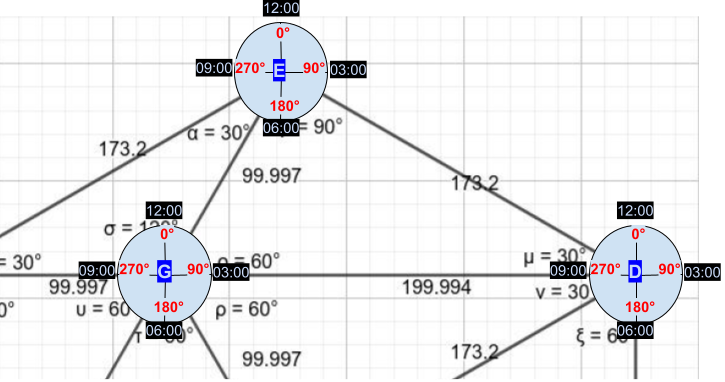
\includegraphics[width=0.95\linewidth]{assets/informatik-prototyp/simulator/internal-angles.png} 
\caption{Winkel im Graph}
\label{fig:labeled-graph-angles}
\end{subfigure}
\begin{subfigure}{0.8\textwidth}
\begin{footnotesize}
\begin{verbatim}

angles = {
    [...],
    'G': {'E': 30, 'D': 90, 'H': 150, 'A': 210, 'F': 270},
    [...],
    }
\end{verbatim}
\end{footnotesize}
\caption{Graph mit Winkeln in YAML Knoten G}
\label{fig:graph-yaml-angle}
\end{subfigure}
\caption{Graph mit Winkeln}
\label{fig:angle-graphs-internal}
\end{figure}

Da der Graph nicht genau so aufgeklebt sein wird wie auf der Skizze, wurden zusätzliche Bereiche definiert, in denen sich die Winkel befinden sollten.

Ein Ausschnitt, der zeigt, wie der interne Graph in einem \gls{yaml} File definiert ist, ist hier eingefügt.

\begin{verbatim}
C: [{D: [0, [30, 120]}, {B: [240, [120, 30]}, {H: 300, [30, 30]}],
\end{verbatim}

Auf Grafik \ref{fig:angled-graph} sind alle Winkel eingezeichnet inklusive der Halbwinkel zwischen allen Kanten. In Grafik \ref{fig:excerpt-angled-graph} ist die Kante zwischen C und D gezeigt, dies entspricht \verb|'C: [{D: [0, [30, 120]}'| im \gls{yaml} File. Da die Linie von C nach D gerade nach oben (nach 12 Uhr) weggeht, ist dies im Idealfall 0\textdegree.
Das der Idealfall nicht eintreten wird, da der Graph nicht perfekt aufgeklebt sein wird und die Linie nicht perfekt in Richtung 12 Uhr gehen wird, sind die Halbwinkel eingezeichnet, hier 30\textdegree\ und 120\textdegree. Die Kante zu Knoten D kann also im Bereich von 0\textdegree-30\textdegree\ und 0\textdegree+120\textdegree, sprich -30\textdegree\ und 180\textdegree\ liegen. Befindet sich eine gemessene Kante in diesem Bereich, wird es die Kante C zu D sein.

\begin{figure}[H]
\centering
\begin{subfigure}{0.65\textwidth}
\centering
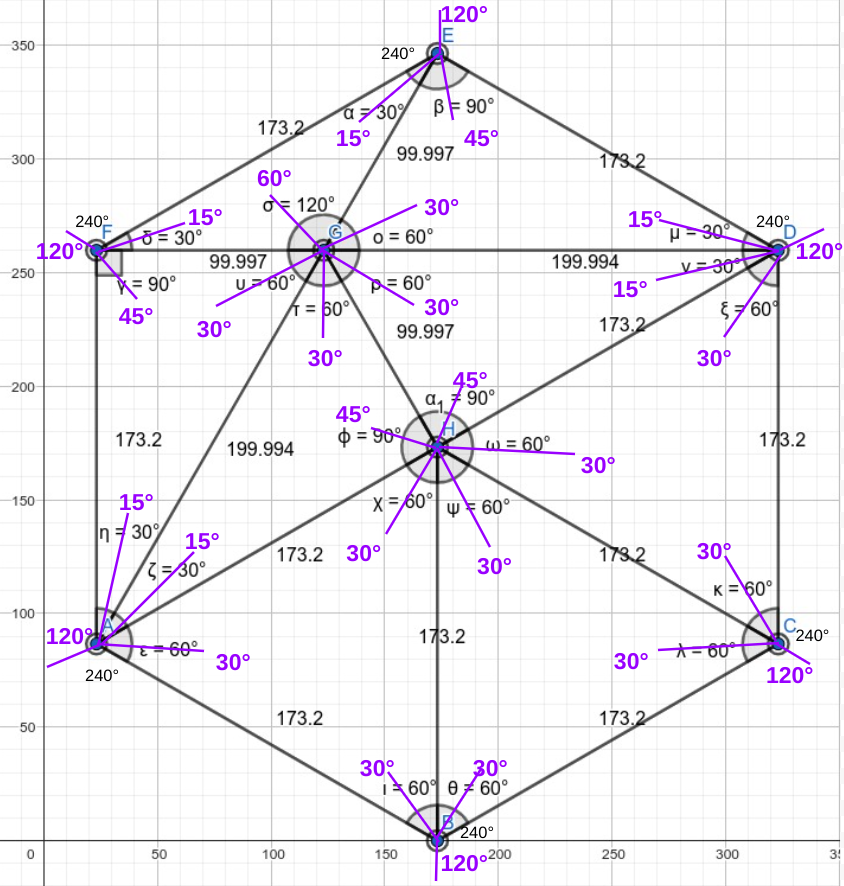
\includegraphics[width=0.95\linewidth]{assets/informatik-prototyp/graph-angles.png} 
\caption{Graph mit Winkeln und Winkelbereichen}
\label{fig:angled-graph}
\end{subfigure}
\begin{subfigure}{0.32\textwidth}
\centering
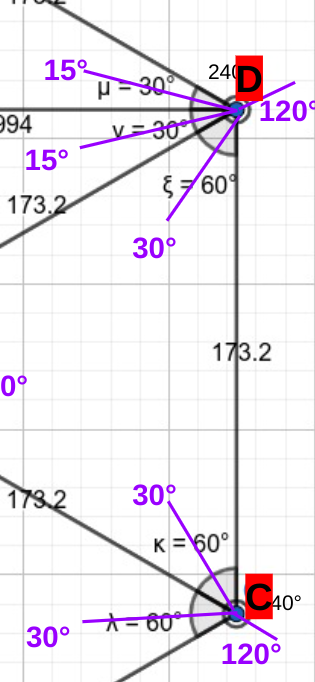
\includegraphics[width=0.95\linewidth]{assets/informatik-prototyp/c-d-angle-labeled.png} 
\caption{C zu D Winkel}
\label{fig:excerpt-angled-graph}
\end{subfigure}
\caption{Winkel und Halbwinkel im Graphen}
\label{fig:angles}
\end{figure}


\subsubsection{Zielknoten erkennen}

Damit der Roboter überprüfen kann, ob er wirklich das Ziel erreicht hat, muss erkannt werden können, ob ein Knoten der richtige Zielknoten ist. Dazu wird der \acrfull{orb} Algorithmus verwendet, der Teil der \gls{opencv} Bibliothek ist. \gls{orb-gloss} lernt die Merkmale von Objekten und erkennt auf einem Bild, welches Objekt gefunden wurde.

Der Algorithmus wird so eingesetzt werden, dass der Roboter bevor er den Lauf beginnt die Merkmale der drei Buchstaben lernt. Jedes Mal, wenn ein Knoten fotografiert wird, um die ausgehenden Kanten zu prüfen, wird ebenfalls geprüft, ob sich ein Buchstaben darauf befindet. Falls ein Buchstaben detektiert wird, bestimmt \acrshort{orb} um welchen es sich handelt.

Dadurch dass \acrshort{orb} die Merkmale der Buchstaben detektiert, ist es nicht nötig, die Rotation der Buchstaben zu beachten. Unabhängig von welcher Richtung der Roboter den Zielknoten fotografiert, kann der Buchstabe erkannt werden.

Auf der folgenden Grafik \ref{fig:orb-zielknoten-konzept} wird mit den farbigen Linien dargestellt, wie \acrshort{orb} die bekannten Merkmale (jeweils linkes Bild) in den zu analysierenden Bildern (jeweils rechtes Bild) findet.

\begin{figure}[H]
\centering
\begin{subfigure}{0.3\textwidth}
\centering
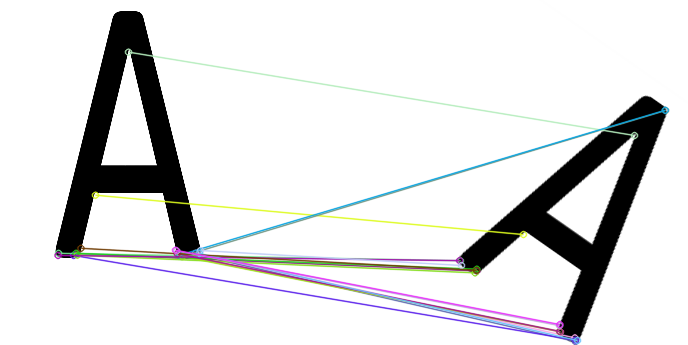
\includegraphics[width=0.95\linewidth]{assets/informatik-prototyp/opencv/target_node_detection/orb-a.png} 
\caption{ORB A}
\label{fig:orb-a-konzept}
\end{subfigure}
\begin{subfigure}{0.3\textwidth}
\centering

\includegraphics[width=0.95\linewidth]{assets/informatik-prototyp/opencv/target_node_detection/orb-b.png} 
\caption{ORB B}
\label{fig:orb-b-konzept}
\end{subfigure}
\begin{subfigure}{0.3\textwidth}
\centering
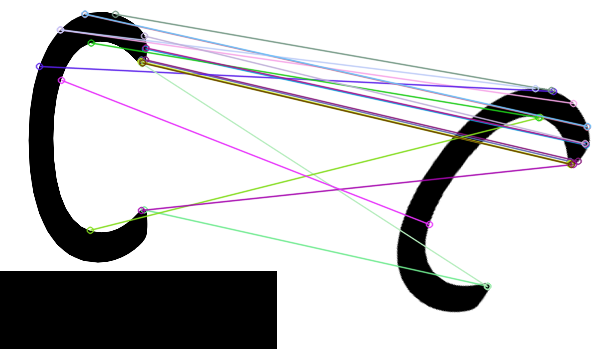
\includegraphics[width=0.95\linewidth]{assets/informatik-prototyp/opencv/target_node_detection/orb-c.png} 
\caption{ORB C}
\label{fig:orb-c-konzept}
\end{subfigure}

\caption{Zielknotenerkennung mit ORB}
\label{fig:orb-zielknoten-konzept}
\end{figure}


Mit \acrshort{orb} werden nur die Buchstaben A, B oder C erkannt, da der trainierte Algorithmus nur diese drei Zeichen kennt. So kann ausgeschlossen werden, dass ein C beispielsweise als das Klammer Zeichen \verb|(| erkannt werden würde.


\subsubsection{Pylonen und Hindernisse erkennen}\label{subsubsection:bilderkennung}

Damit der Roboter weiss, ob sich eine Pylone auf einem Nachbarsknoten oder eine Barriere auf einer ausgehenden Linie befindet, wird der Ablauf auf Abbildung \ref{fig:image-detection-obstacles} durchgeführt.

\begin{figure}[H]
\centering
\begin{subfigure}{0.45\textwidth}
\centering
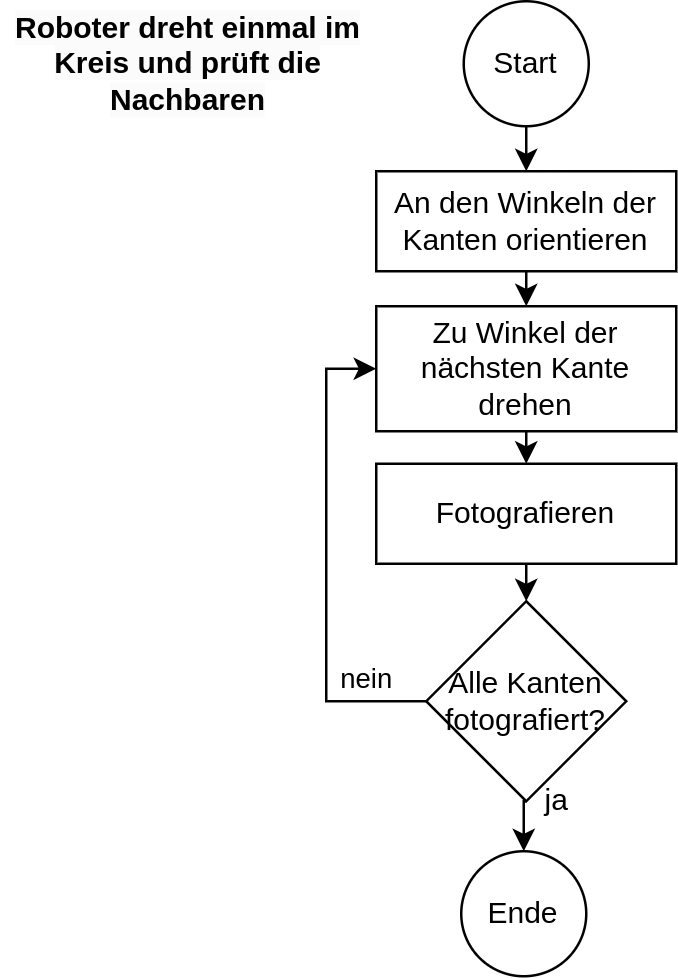
\includegraphics[width=0.95\textwidth]{assets/gesamtkonzept/ablaufdiagramm-hindernisse-erkennen.png}
\caption{Ablaufdiagramm Hindernis erkennen}
\label{fig:ablaufdiagramm-hindernis-erkennen}
\end{subfigure}
\begin{subfigure}{0.5\textwidth}
\centering
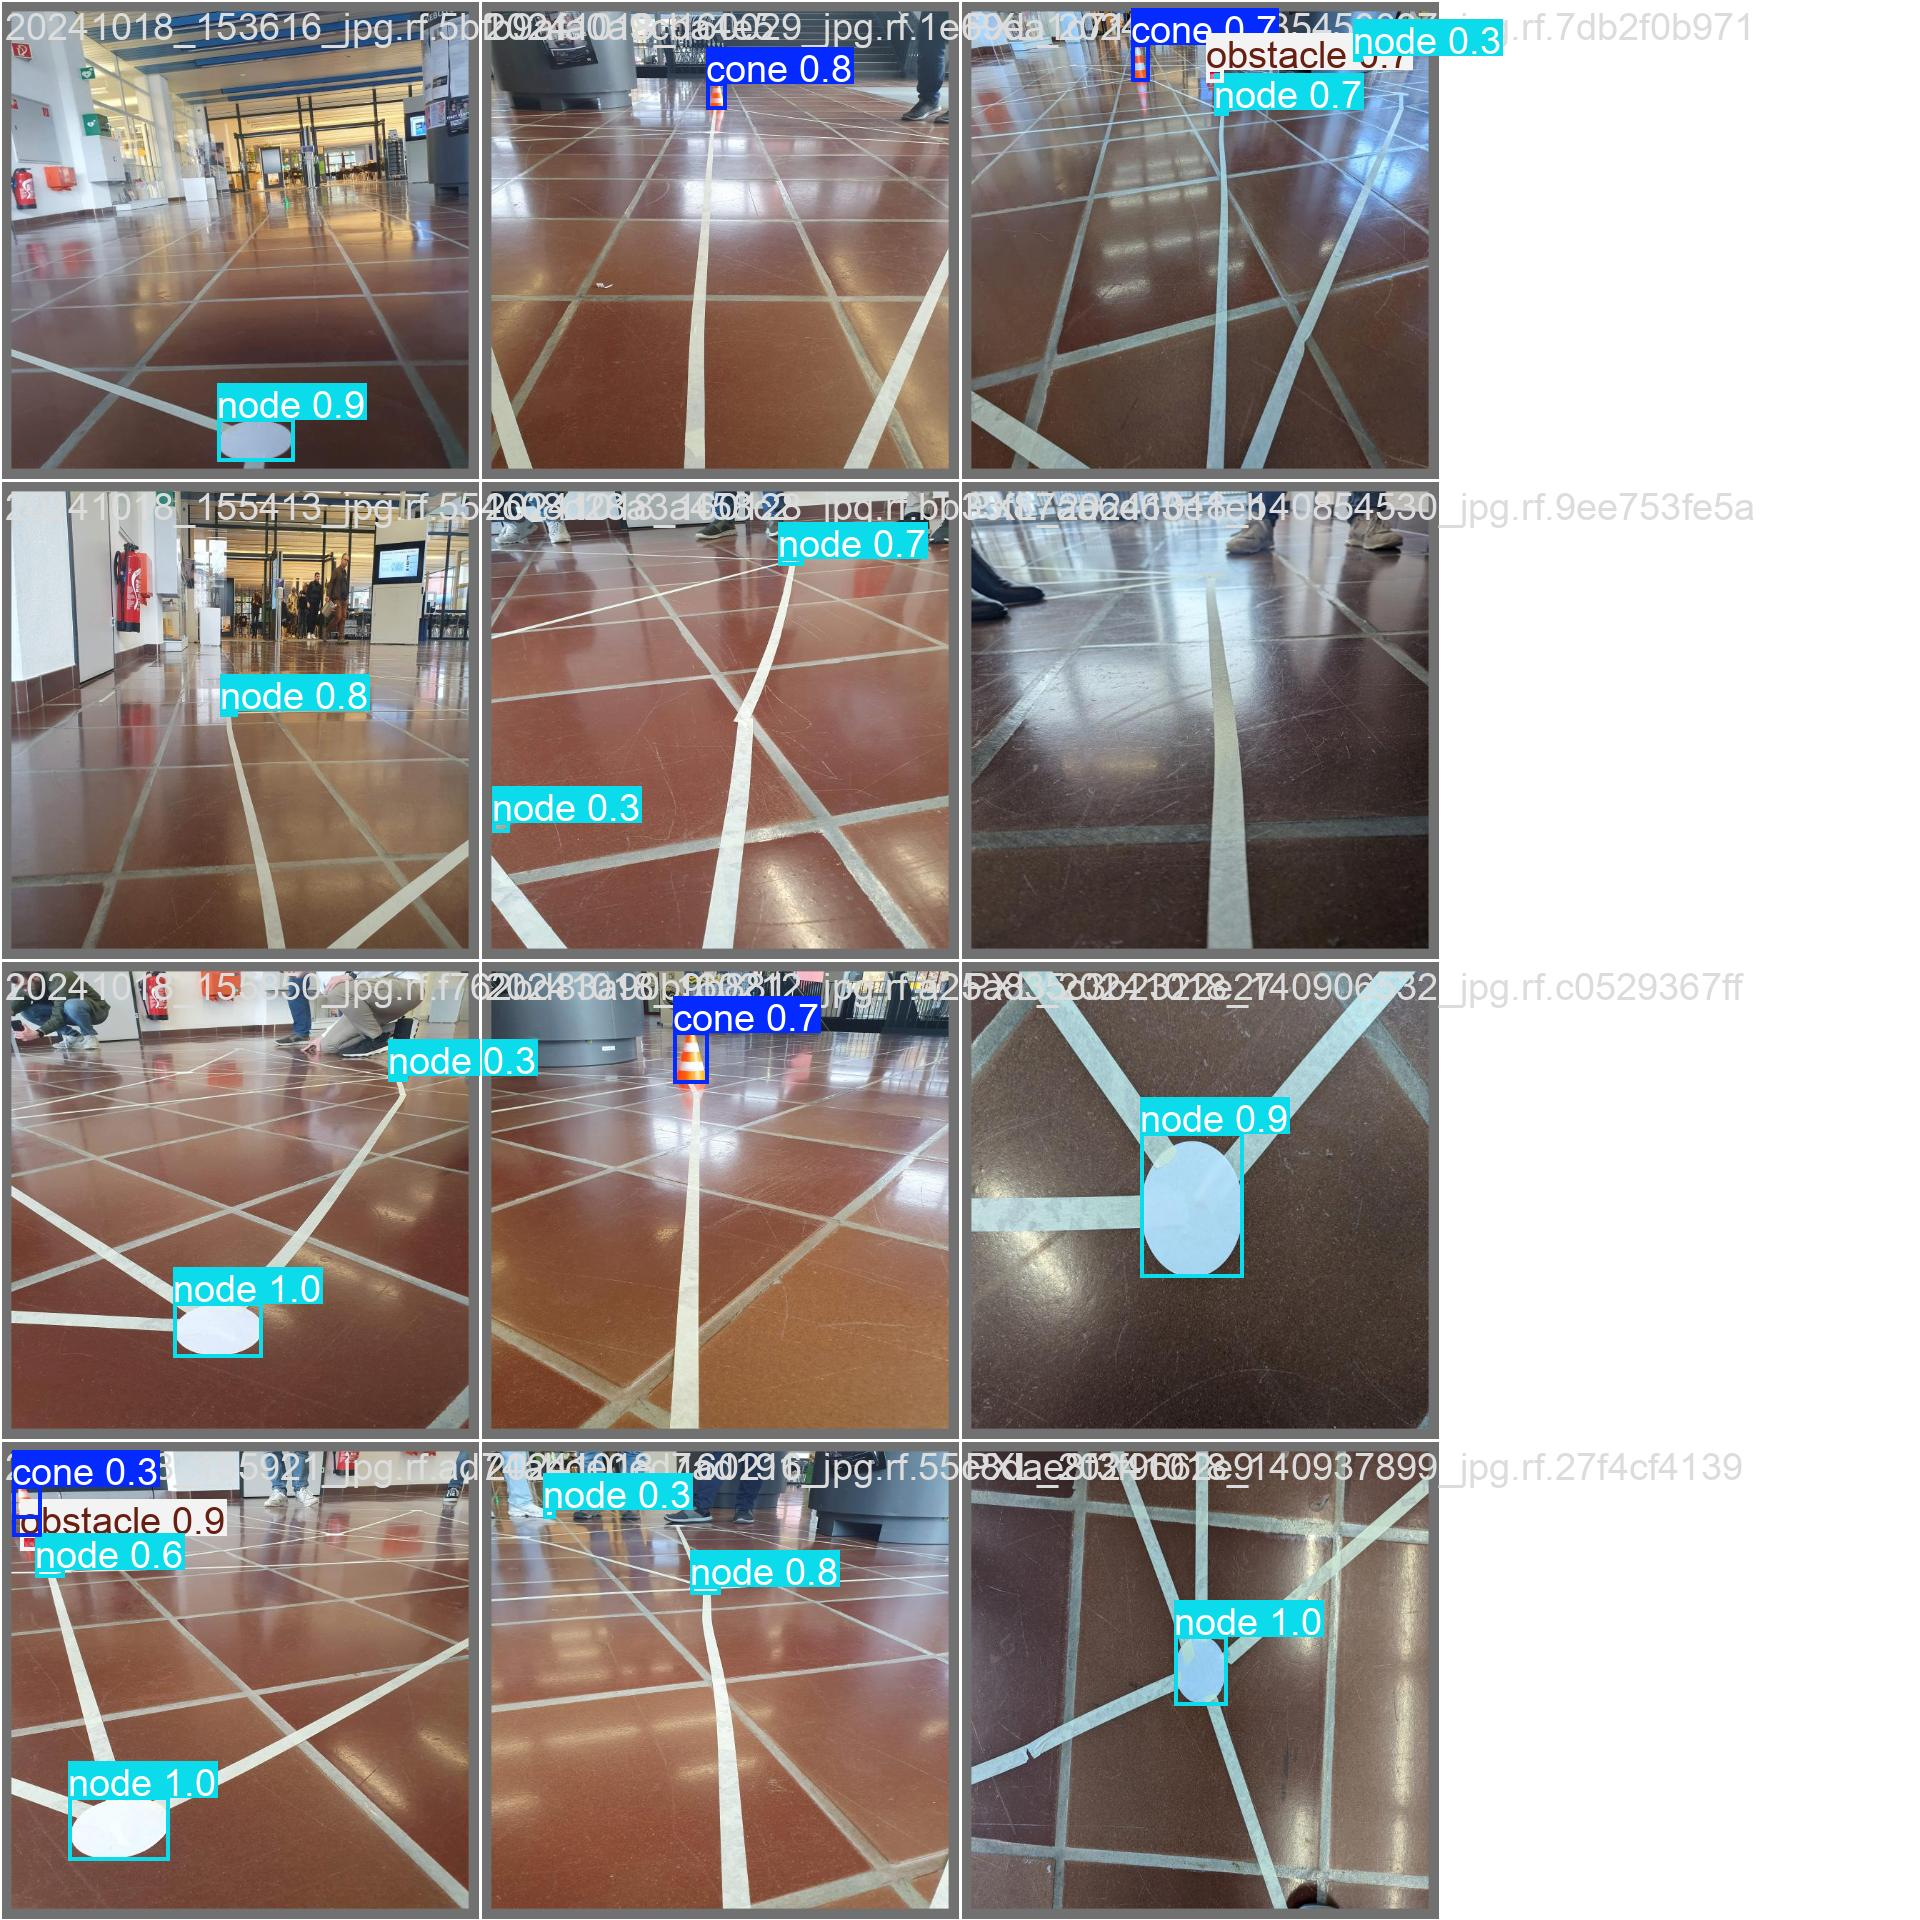
\includegraphics[width=0.95\textwidth]{assets/informatik-prototyp/yolo/recognized-images.jpeg}
\caption{YOLOv11 Bilderkennung}
\label{fig:img-recognition-yolo-concept}
\end{subfigure}
\caption{Bilderkennung Hindernisse}
\label{fig:image-detection-obstacles}
\end{figure}

Aus dem vorherigen Schritt des Winkelerkennens, kennt der Roboter alle ausgehenden Linien und deren Position. Er dreht sich nun im Uhrzeigersinn zu jeder Kante und fotografiert diese. Durch das Hochformat der Kameras sieht er weit in die Ferne und kann auch nur die wichtigen Elemente sehen, sprich, diese, die sich auf der Linie befinden.

Die Bilder werden mit dem \gls{yolo} Objekterkennungsalgorithmus ausgewertet. Dabei werden sowohl Knoten, als auch Pylonen und Barrieren erkannt. Das erhaltene Resultat beschreibt anhand der definierten Klassen, welche Elemente erkannt wurden und mithilfe der Koordinaten, wo sich diese auf dem Bild befinden.
Alle Hindernisse werden intern gespeichert indem die jeweiligen Kanten höher gewichtet oder Knoten entfernt werden.


\newpage

\subsubsection{Hindernisse bewegen}
\label{subsubsection:Hindernisse bewegen}

Um ein vorhandenes Hindernis zu bewegen, wird ein Mechanismus zum Anheben, nachfolgend Greifer genannt, verwendet. Nach dem Anheben bewegt sich der Roboter und setzt das Hindernis an der alten Position ab.
Mit nur einem Motor wird das Hindernis eingeklemmt, zentriert und angehoben. Dieser Vorgang und der Aufbau des Greifers wird in folgendem Kapitel erläutert.

Die gezeigten Abbildungen des Greifers stammen von einem Prototyp und stellen nicht das finale Design dar. Sie dienen lediglich zur Veranschaulichung der Funktionsweise. Die Dimensionen des Gestänges sowie die Positionen der Lagerstellen sollen für die finale Variante beibehalten werden.

In der Nutzwertanalyse (Anhang \nameref{nutzwertanalyse}) hat man sich zum Anheben des Hindernisses für ein Klemm-Design entschieden, welcher das Hindernis oben an der längsten Kante an 3 Punkten einspannt (siehe Abb. \ref{fig:obstacle_clamping_concept}). 


\begin{figure}[H]
\centering
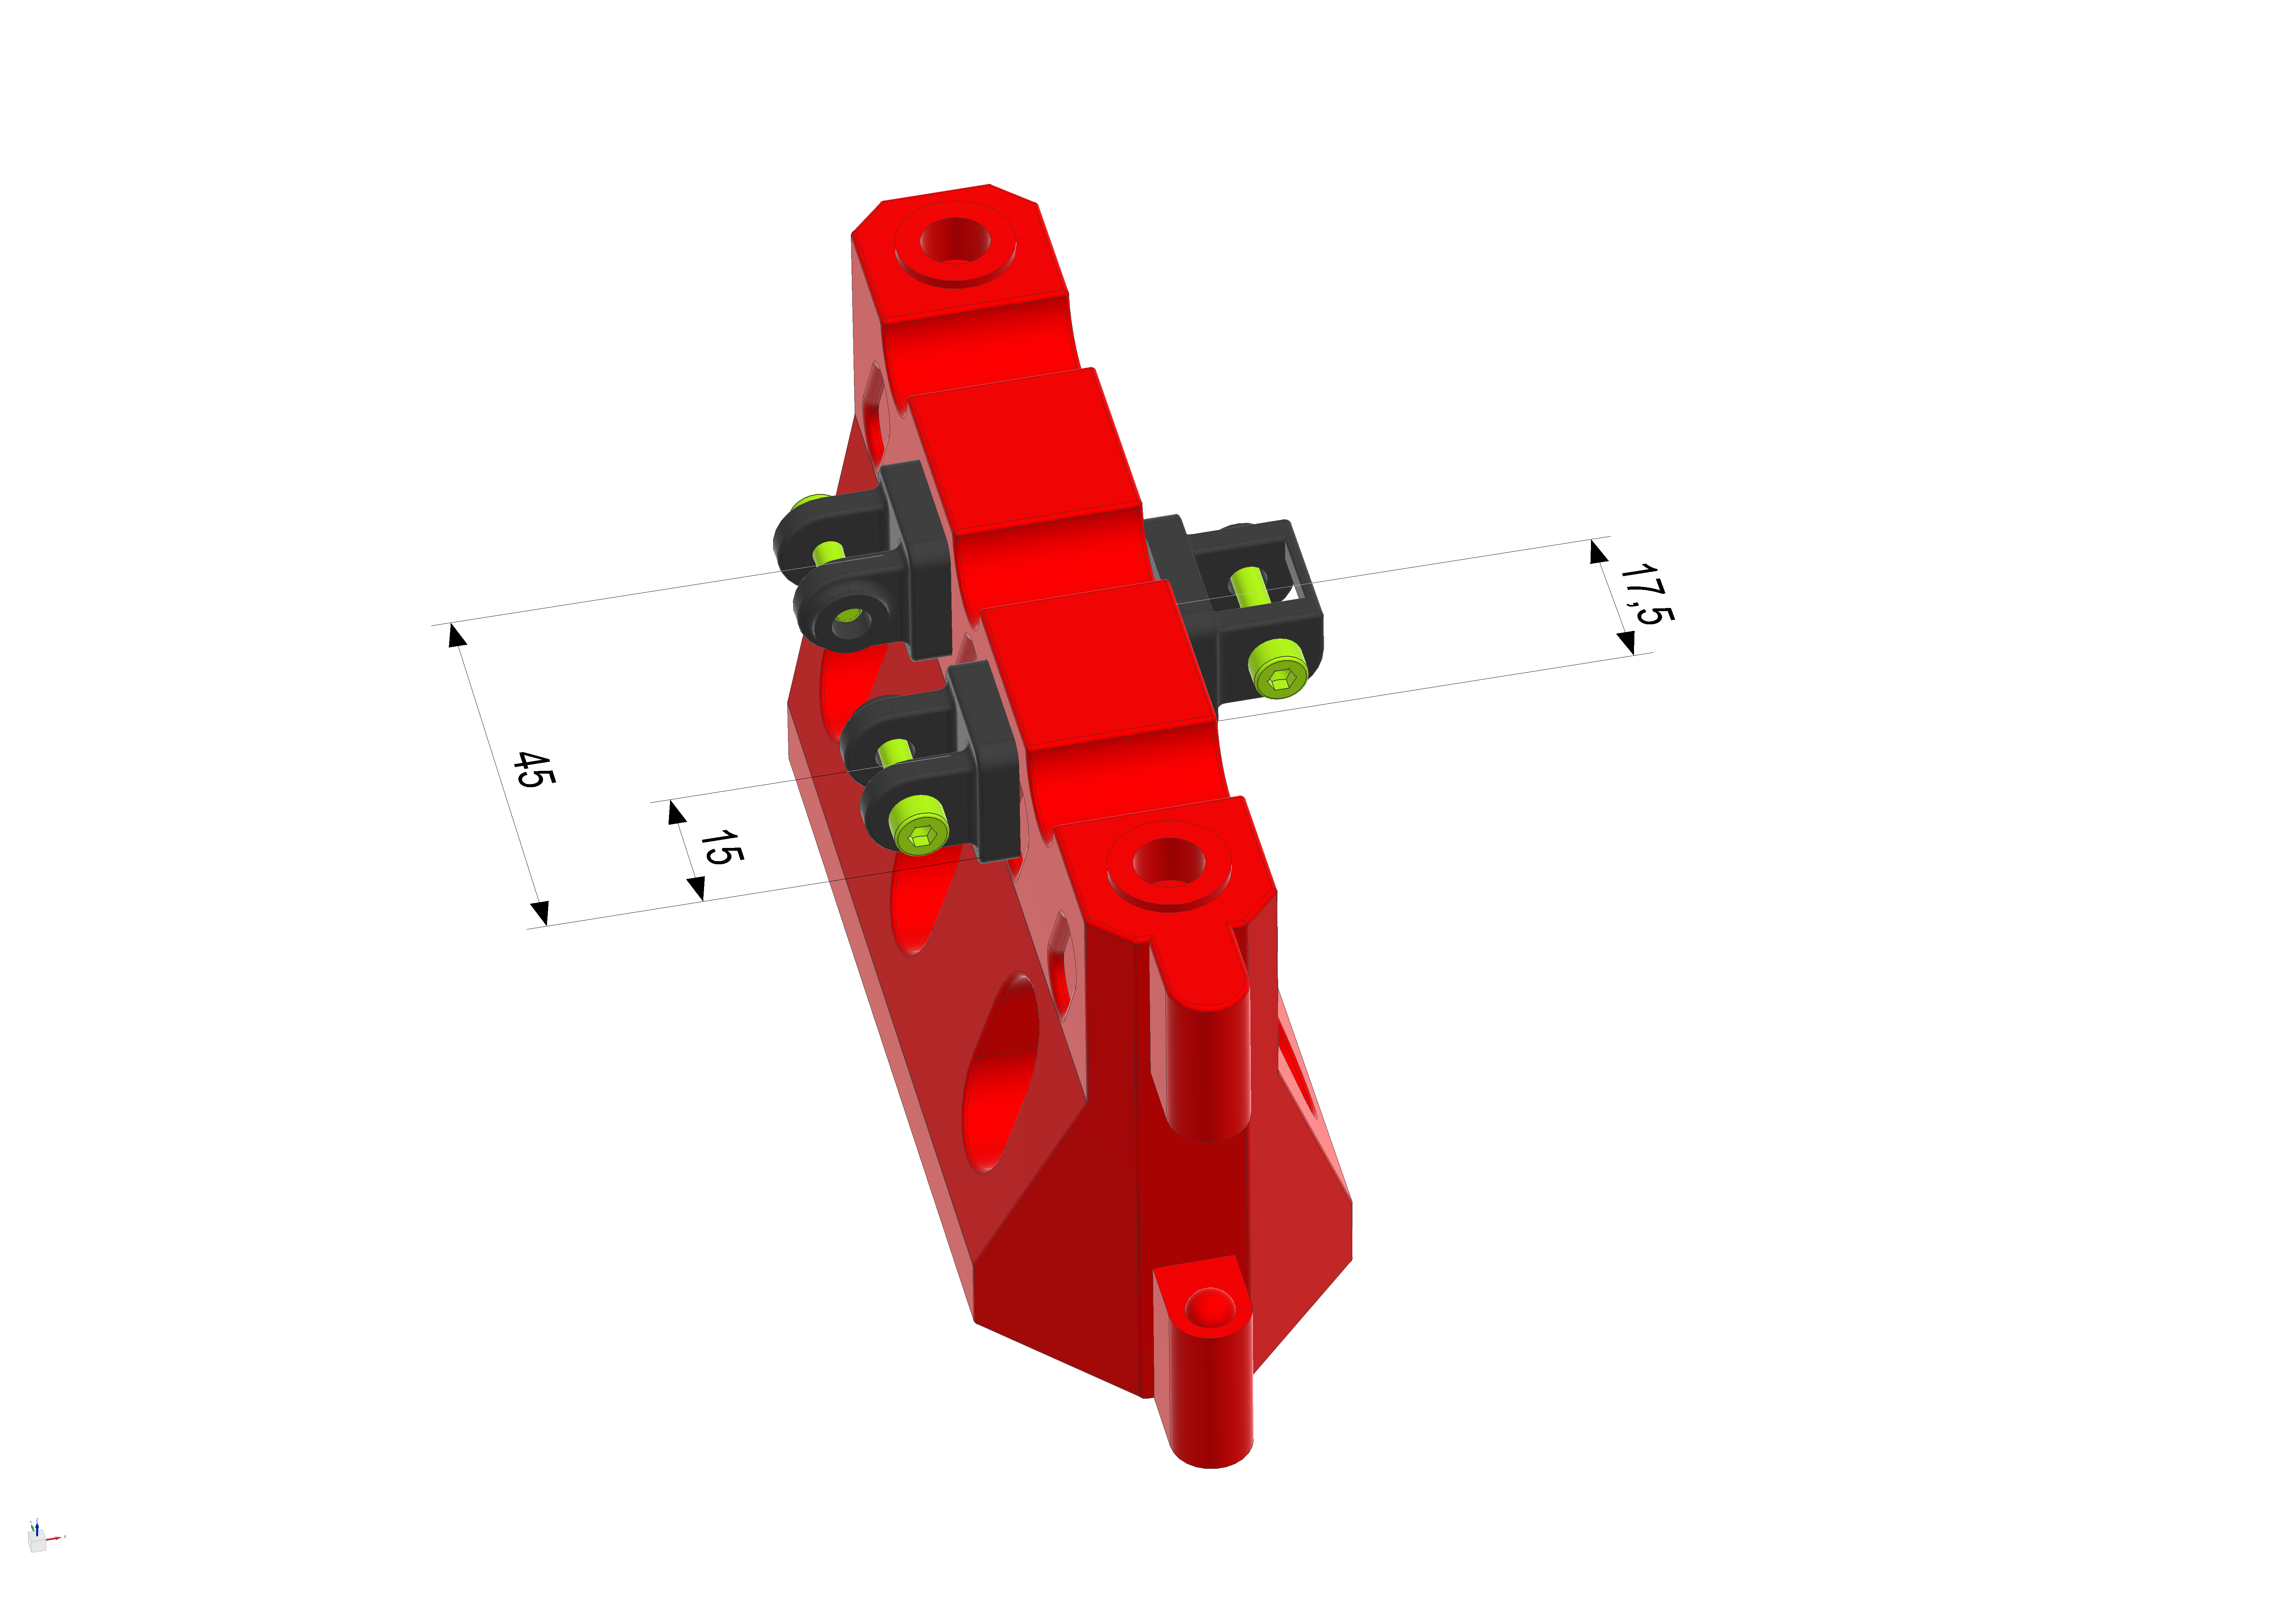
\includegraphics[width=0.95\linewidth]{assets/greifer-prototyp/Greifer_Backen_Trimetric.png} 
\caption{Position Klemmbacken}
\label{fig:obstacle_clamping_concept}
\end{figure}

\newpage

Um sowohl das Klemmen, als auch das Anheben des Hindernisses mit einem einzelnen Servomotor zu realisieren, wurde der Mechanismus als ein Gestänge realisiert (Abb. \ref{fig:gripper_components}).

\begin{figure}[H]
\centering
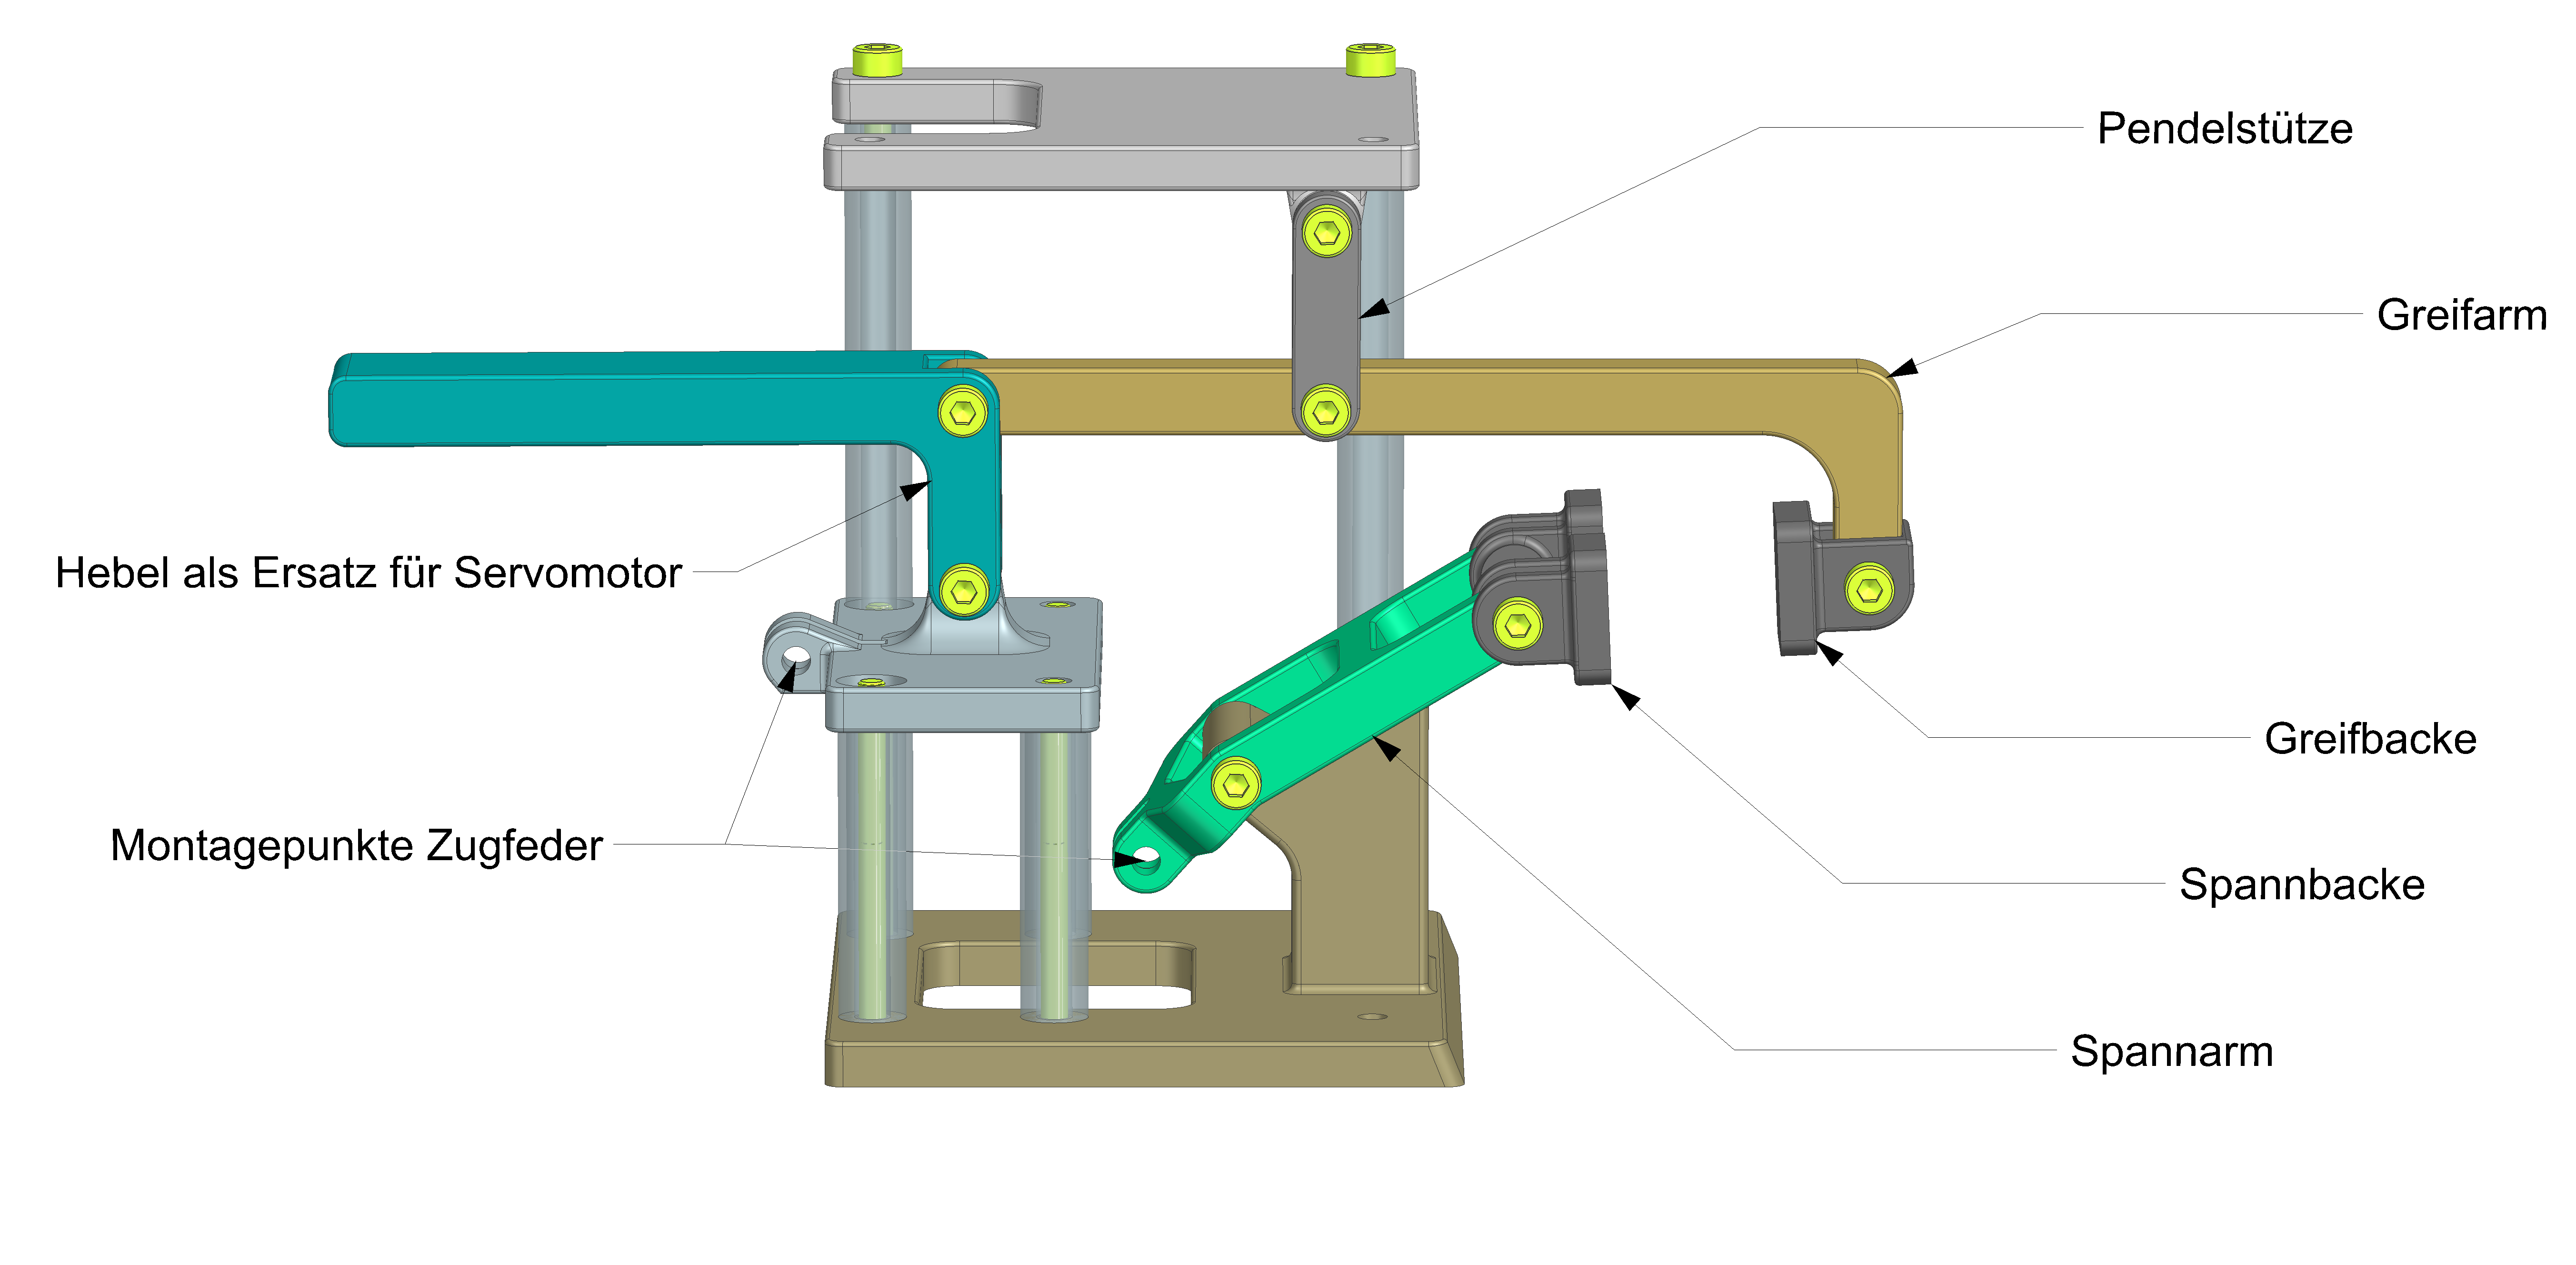
\includegraphics[width=1.0\linewidth]{assets/greifer-prototyp/Greifer_side_Komponentennamen.png} 
\caption{Komponenten des Greifers}
\label{fig:gripper_components}
\end{figure}

Die Greifbacke ist gelenkig mit dem Greifarm verbunden, welcher von der Pendelstütze geführt wird. Am Ende des Greifarms wird der Arm des Servomotors befestigt. Der Servomotor ist in der Abbildung durch einen Hebel ersetzt, da der Prototyp zu Beginn des Prototypings von Hand bedient wird. Die zwei Spannbacken sind am Spannarm befestigt. Dieser Spannarm ist drehbar am Chassis des Fahrzeugs gelagert und wird durch eine Zugfeder vorgespannt. Abgebildet sind nur die Montagepunkte der Feder.

\newpage

Dreht der Servomotor im Uhrzeigersinn, so schwingen Greifarm und Greifbacke nach oben weg. Der Greifer ist geöffnet (Abb. \ref{fig:gripper_opening_side}). So kann der Roboter auf das Hindernis zu fahren, bis dieses die zwei Spannbacken berührt. An beiden Spannbacken wird jeweils ein Endschalter montiert, welcher erkennt, wann das Hindernis nahe genug ist und anschliessend den Hebeprozess startet. Dieser Endschalter ist auf der Abbildung \ref{fig:gripper_opening_side} nicht ersichtlich.

Dreht der Servomotor aus dieser Position im Gegenuhrzeigersinn, so schwingt die Greifbacke zurück, bis sie in Berührung mit dem Hindernis kommt. Dadurch wird das Hindernis gegen die zwei Spannbacken gedrückt, welche wiederum durch die Vorspannung der Feder gegen das Hindernis drücken. Das Hindernis wird eingeklemmt (Abb. \ref{fig:gripper_gripping_side}).

Dreht der Servomotor weiter im Gegenuhrzeigersinn, so dreht nun auch der Spannarm im Gegenuhrzeigersinn mit, da er über das Hindernis vom Greifarm bewegt wird. Die Rotation des Spannarms führt dazu, dass das Hindernis angehoben wird (Abb. \ref{fig:gripper_lifting_side}). Gleichzeitig wird durch die Rotation des Spannarms die Zugfeder leicht verlängert. Somit wird die Klemmkraft auf das Hindernis erhöht und sichergestellt, dass dieses nicht aus dem Greifer rutscht.

\begin{figure}[H]
\centering
\begin{subfigure}{0.49\textwidth}
\centering
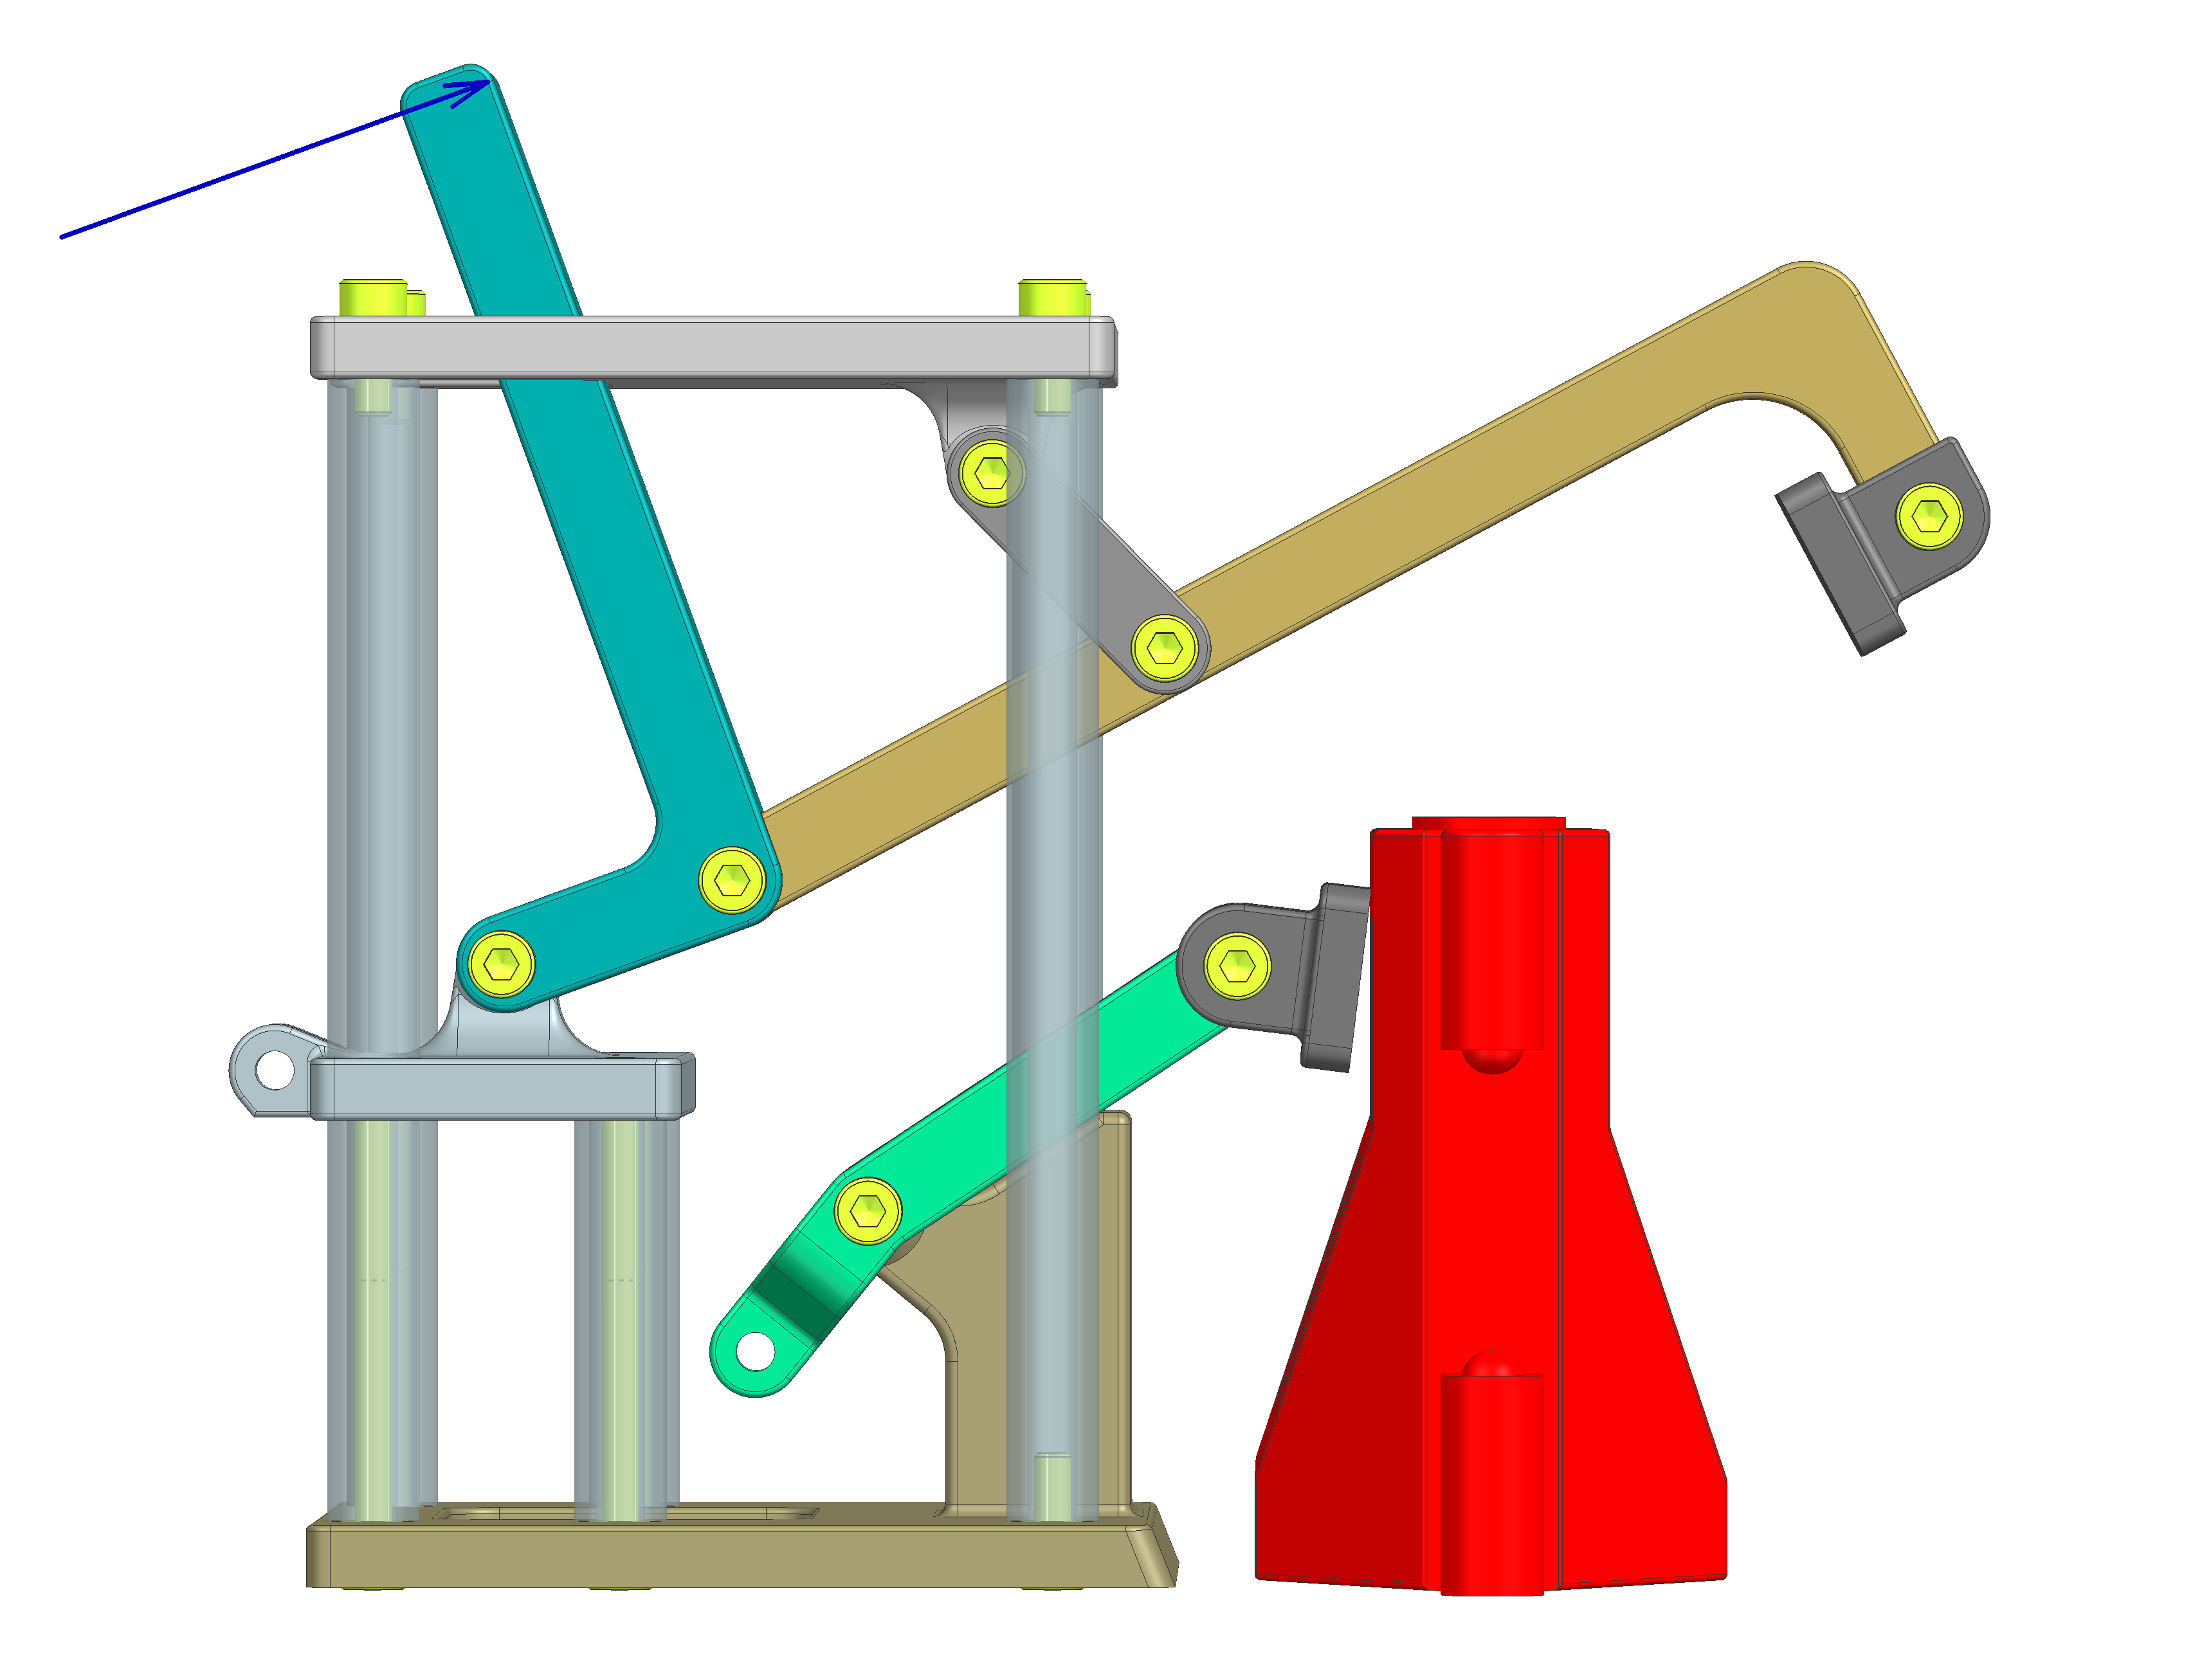
\includegraphics[width=\textwidth]{assets/greifer-prototyp/Greifer_side_Offen.png}
\caption{öffnen}
\label{fig:gripper_opening_side}
\end{subfigure}
\begin{subfigure}{0.49\textwidth}
\centering
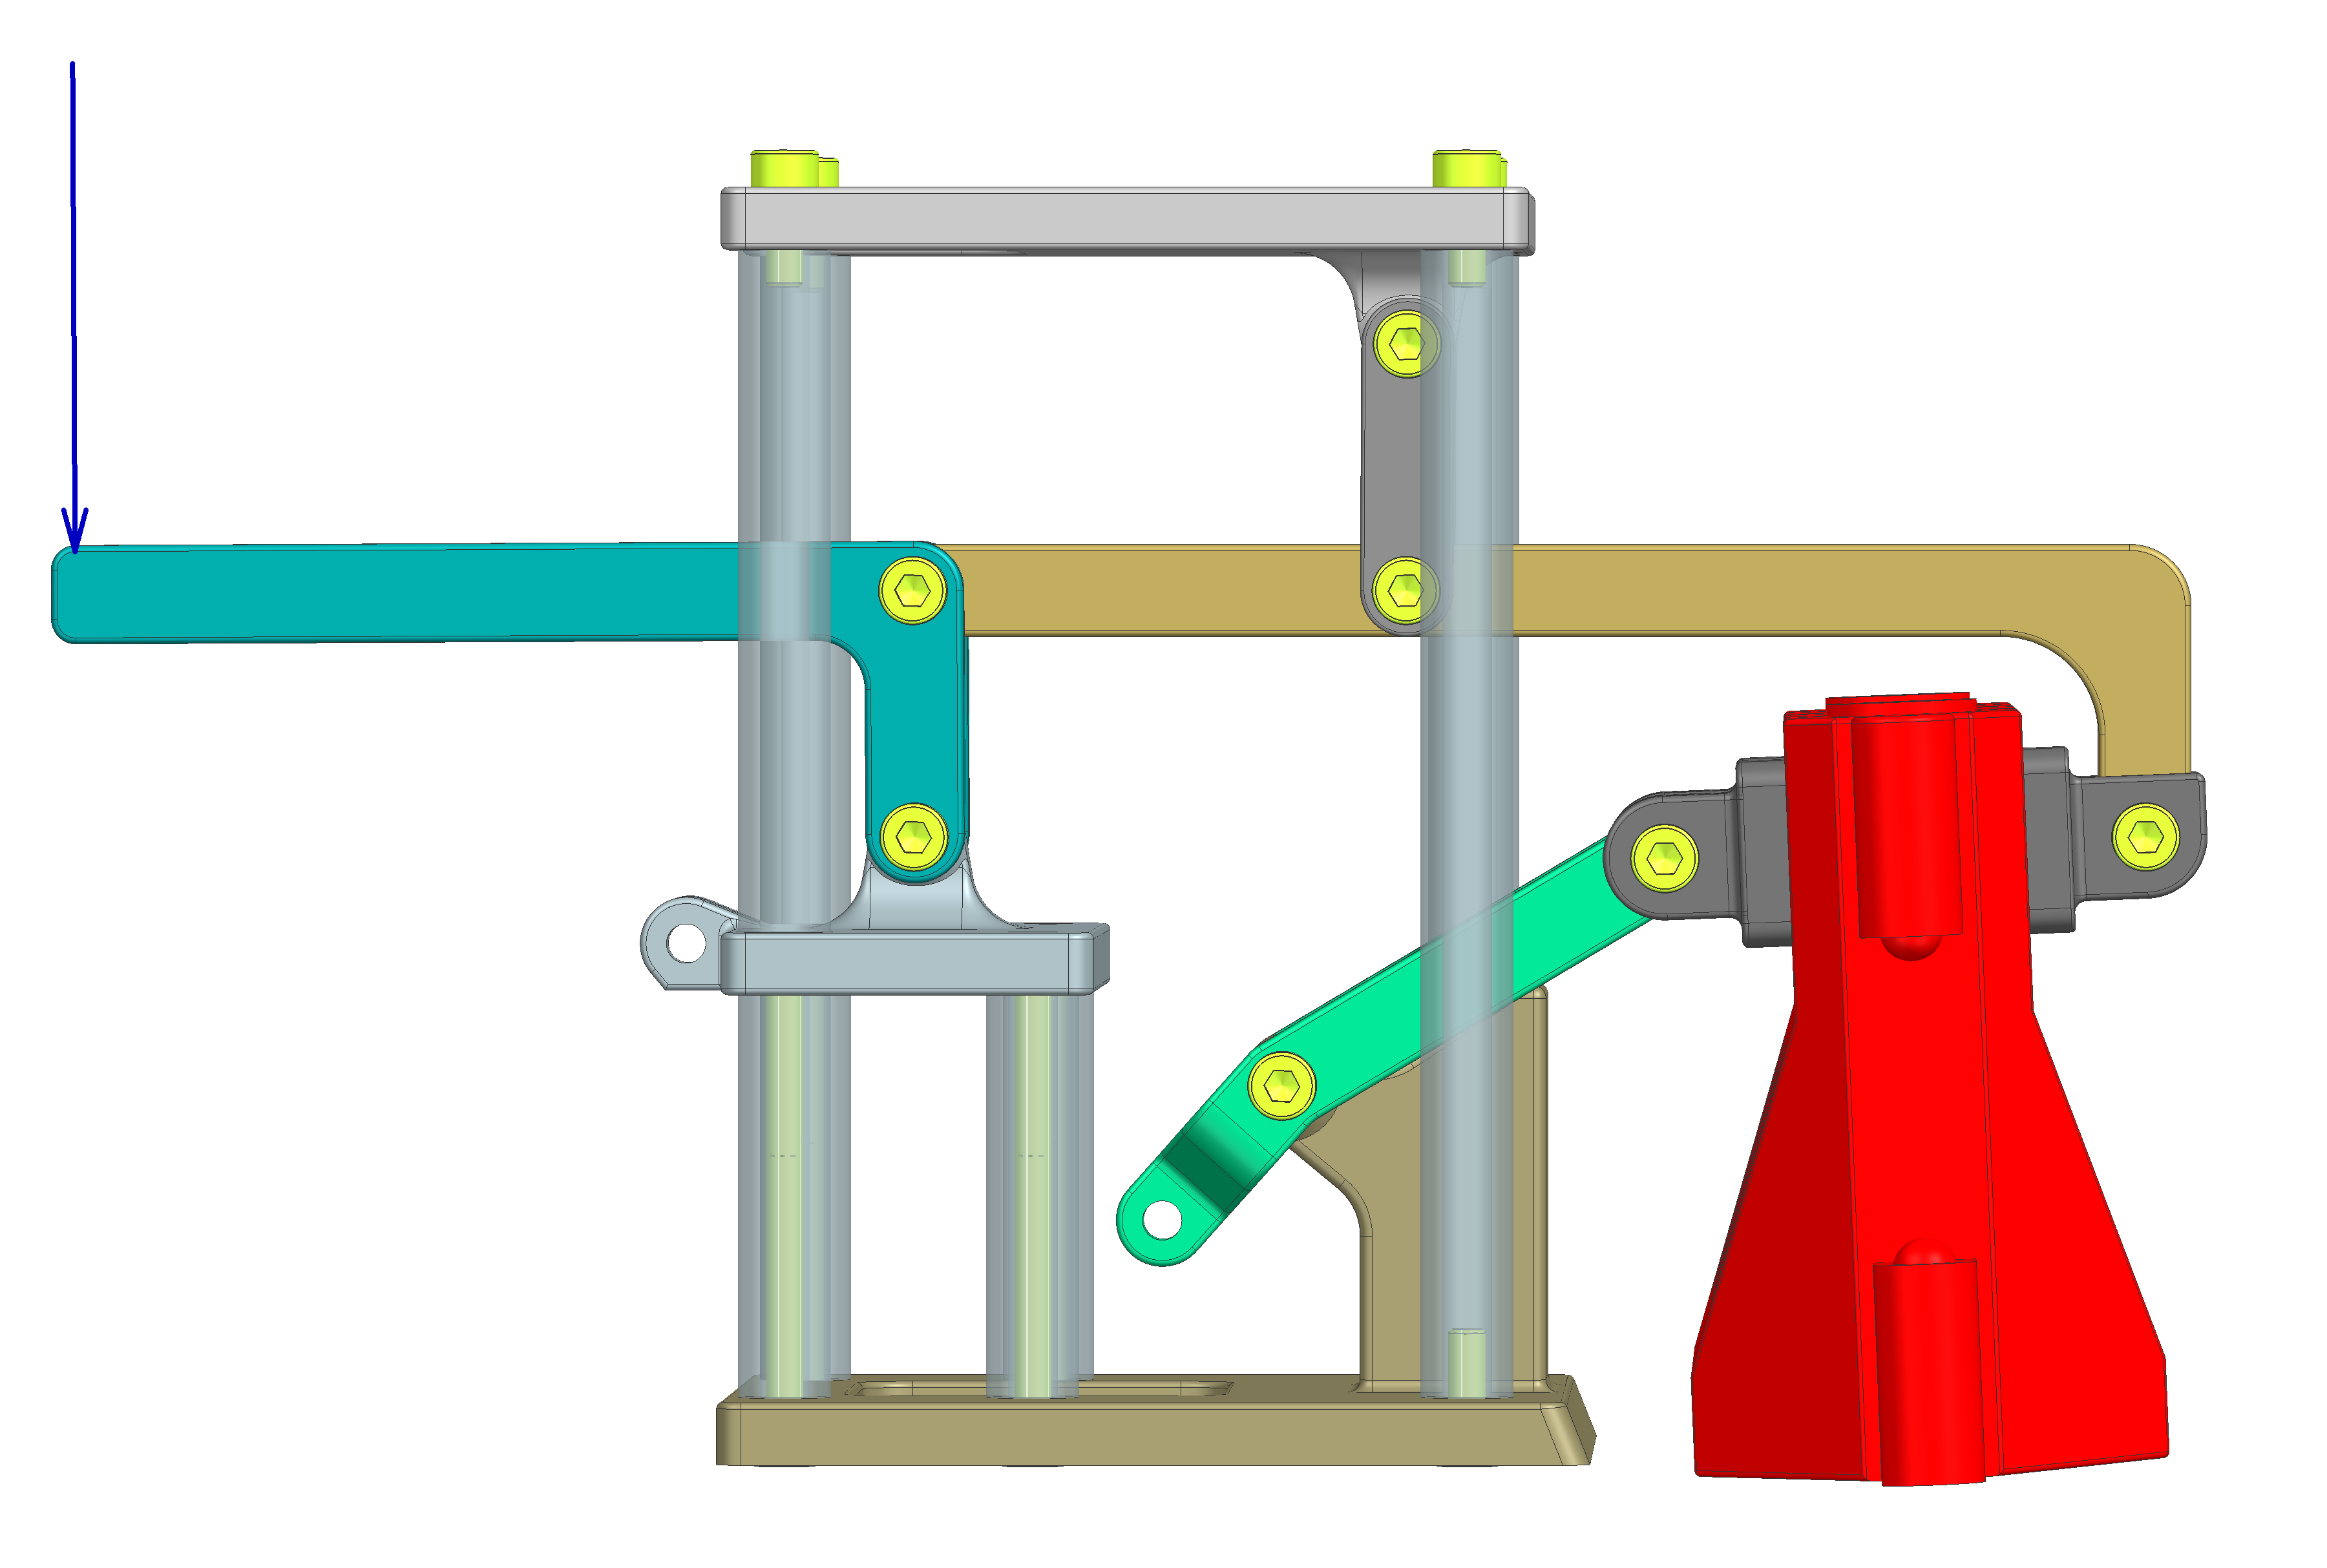
\includegraphics[width=\textwidth]{assets/greifer-prototyp/Greifer_side_Klemmen.png}
\caption{klemmen}
\label{fig:gripper_gripping_side}
\end{subfigure}
\begin{subfigure}{0.49\textwidth}
\centering
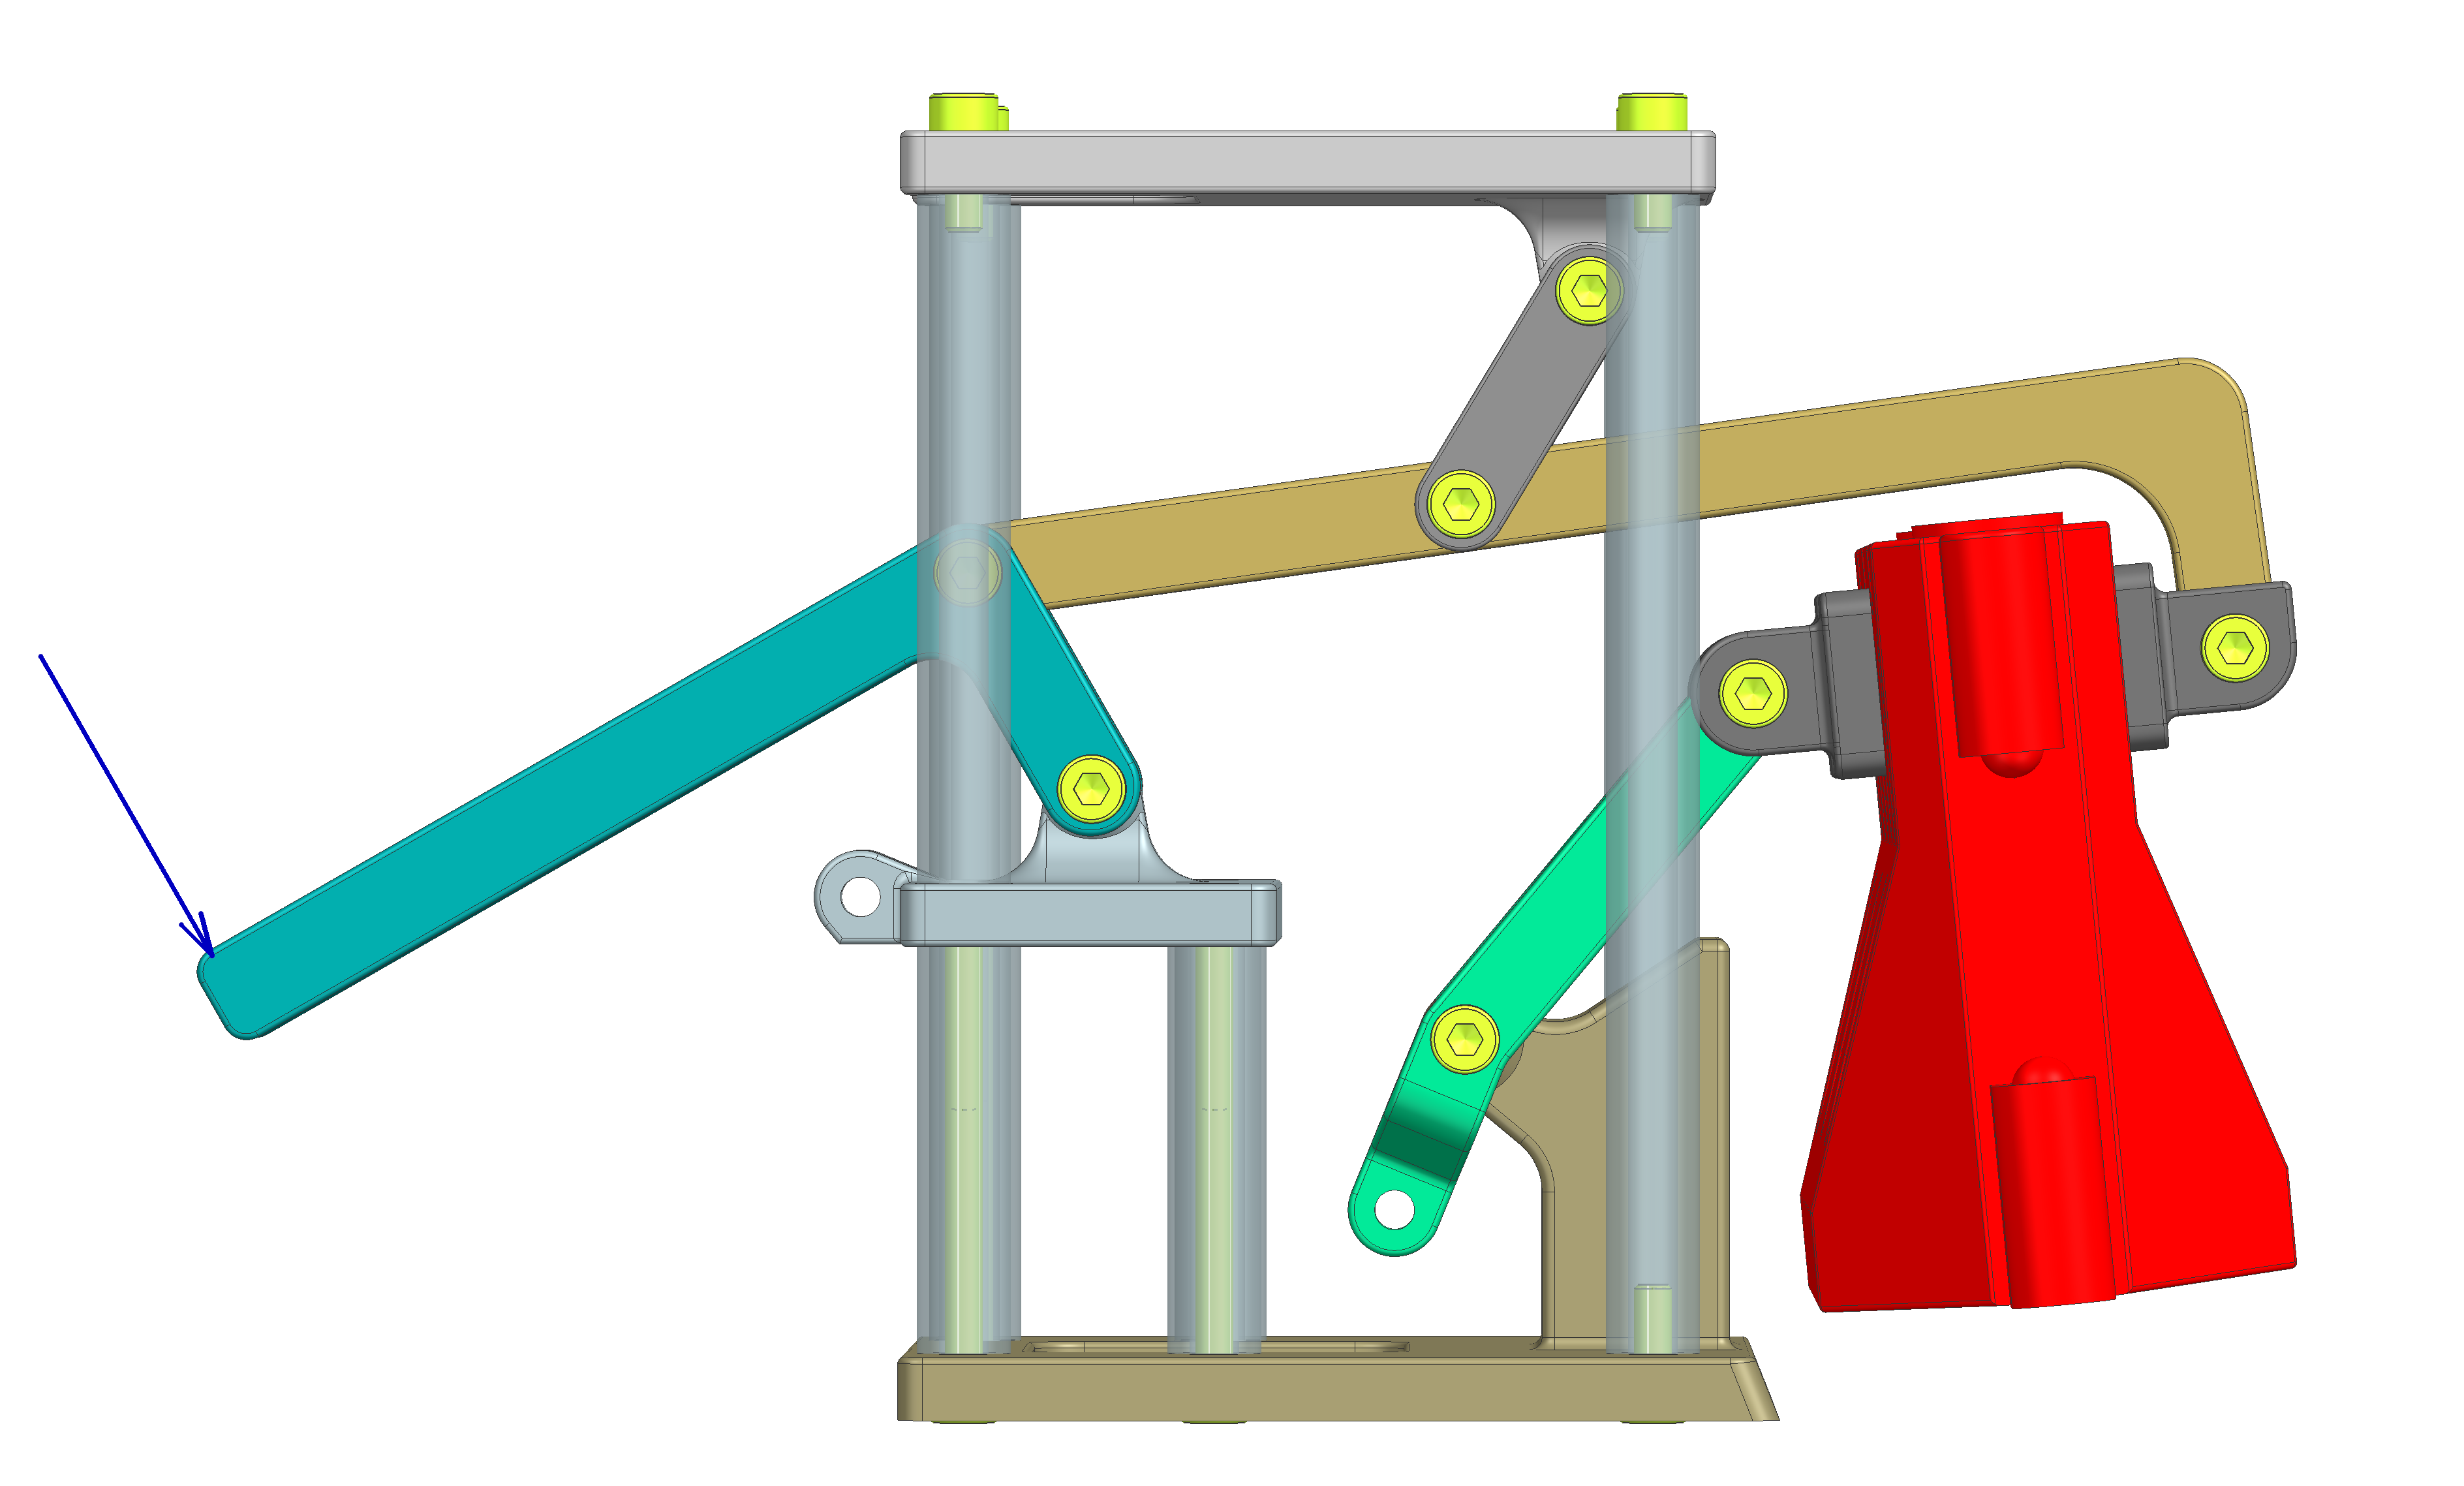
\includegraphics[width=\textwidth]{assets/greifer-prototyp/Greifer_side_Angehoben.png}
\caption{anheben}
\label{fig:gripper_lifting_side}
\end{subfigure}
\caption{Ablauf Hindernis anheben}
\label{fig:obstacle_gripping_process}
\end{figure}

 \newpage
 
Als Basis zur Auslegung des Greifers dient eine Berechnung der nötigen Klemmkraft, um das Hindernis anzuheben. Dazu wurden ein Haftreibwert von 0.3 zwischen Hindernis und Klemmbacken und eine Sicherheit gegen das Rutschen von 1.5 angenommen. Mit der Klemmkraft konnte anhand der Geometrie des Greifers eine Feder mit ausreichend hoher Federkonstante ausgewählt werden. Schliesslich wurde zur Auswahl des Servomotors das nötige Drehmoment berechnet, um sowohl die Zugfeder zu verlängern, als auch das Hindernis anzuheben. Die detaillierten Berechnungen sind im Kapitel \nameref{subsubsection:gripper-calculations} zu finden. Die Ergebnisse aus den Berechnungen wurden im Kapitel \nameref{subsubsection:gripper-prototype-1} anhand eines Prototyps validiert.

Das Klemmen und Anheben ist nur ein Teilschritt  zur Beseitigung eines Hindernisses. Nachfolgend wird der gesamte Ablauf erläutert. Ausgangslage bildet der Ultraschallsensor, der das Hindernis erkannt hat und den Prozess einleitet. 

\begin{figure}[H]
\centering
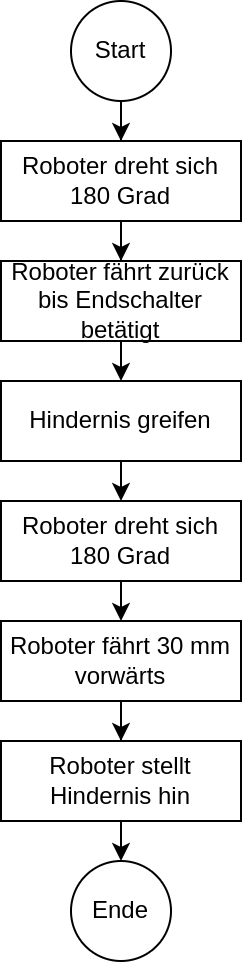
\includegraphics[width=0.2\textwidth]{assets/gesamtkonzept/ablaufdiagramm-hindernis-bewegen.png}
\caption{Ablaufdiagramm Hindernis bewegen}
\label{fig:ablaufdiagramm-hindernis-bewegen}
\end{figure}

 Mit einem Ultraschall-Sensor soll das Vorhandensein eines Hindernisses und die ungefähre Distanz dazu bestimmt werden. Zur genauen Bestimmung der Distanz vor dem Greifer wird der Endschalter am Greifmechanismus verwendet.
Greifer und Endschalter werden sich an der Rückseite des Fahrzeugs befinden, der Ultraschallsensor vorne (siehe Abb. \ref{fig:robot_concept-scetch_labeld}). Dadurch muss sich das Fahrzeug, nachdem ein Hindernis mittels Ultraschall entdeckt wurde, 180\textdegree\ drehen und langsam rückwärts fahren, bis der Endschalter am Greifer betätigt wird, um das Hindernis anzuheben. Sobald das Hindernis angehoben ist, dreht sich das Fahrzeug 180\textdegree\ und fährt 30mm vorwärts, um das Hindernis an dieselbe Stelle zurückzusetzen. Das Fahrzeug steht nach dem Absetzen wieder nach vorne ausgerichtet und kann geradeaus weiter fahren (siehe  Abb. \ref{fig:ablaufdiagramm-hindernis-bewegen}).


\subsection{Fahrwerk}

Auf Basis der Nutzwertanalyse, wurde anschliessend ein Konzept für das Fahrwerk konstruiert. Dies beinhaltet alle Elemente wie Motoren, Akkus, Liniensensoren und Steuerungseinheiten, die für selbständige Fortbewegung notwendig sind. Dafür wurde ein Prototyp erstellt. Bei diesem Prototyp stand der einfache und zweckmässige Aufbau im Vordergrund. Bei der Grundplatte wurde darauf geachtet, dass verschiedene  Versionen von Systemen einfach aufgebaut und ausgetauscht werden können. Ein flexibler Prototyp ist ressourcenschonend. Mehr Informationen dazu gibt es im Kapitel \ref{section:Nachhaltigkeit} Nachhaltigkeit. 

Das Fahrwerk wird wie in Abbildung  \ref{fig:Prototype_Fahrwerk_CAD} gezeigt aufgebaut. Das Fahrzeug wird mit zwei einzeln angesteuerten Räder angetrieben. Damit wird sowohl das Vorwärtsfahren, als auch das Drehen der Räder durchgeführt. Zusätzlich zu den beiden angetriebenen Rädern besitzt das Fahrzeug ein frei-drehendes Abstützrad. Direkt vor dem Abstützrad wird der Distanzsensor montiert. (Kap. \ref{subsection:Distanzsensor} Distanzsensor). Die \acrfull{dc} Motoren besitzen Encoder und sind über eine Welle direkt mit den Antriebsrädern verbunden (Abb. \ref{fig:sectionview-wheelmount}). Dadurch kann genau festgestellt werden, welche Distanz zurückgelegt wurde. Der Fahrbefehl entsteht aufgrund der Berechnungen der Bilderkennung. Dem Mikrocontroller \gls{tinyk22}, der die Motoren ansteuert, werden Distanz und Drehwinkel mitgeteilt. 

\begin{figure}[H]
\centering
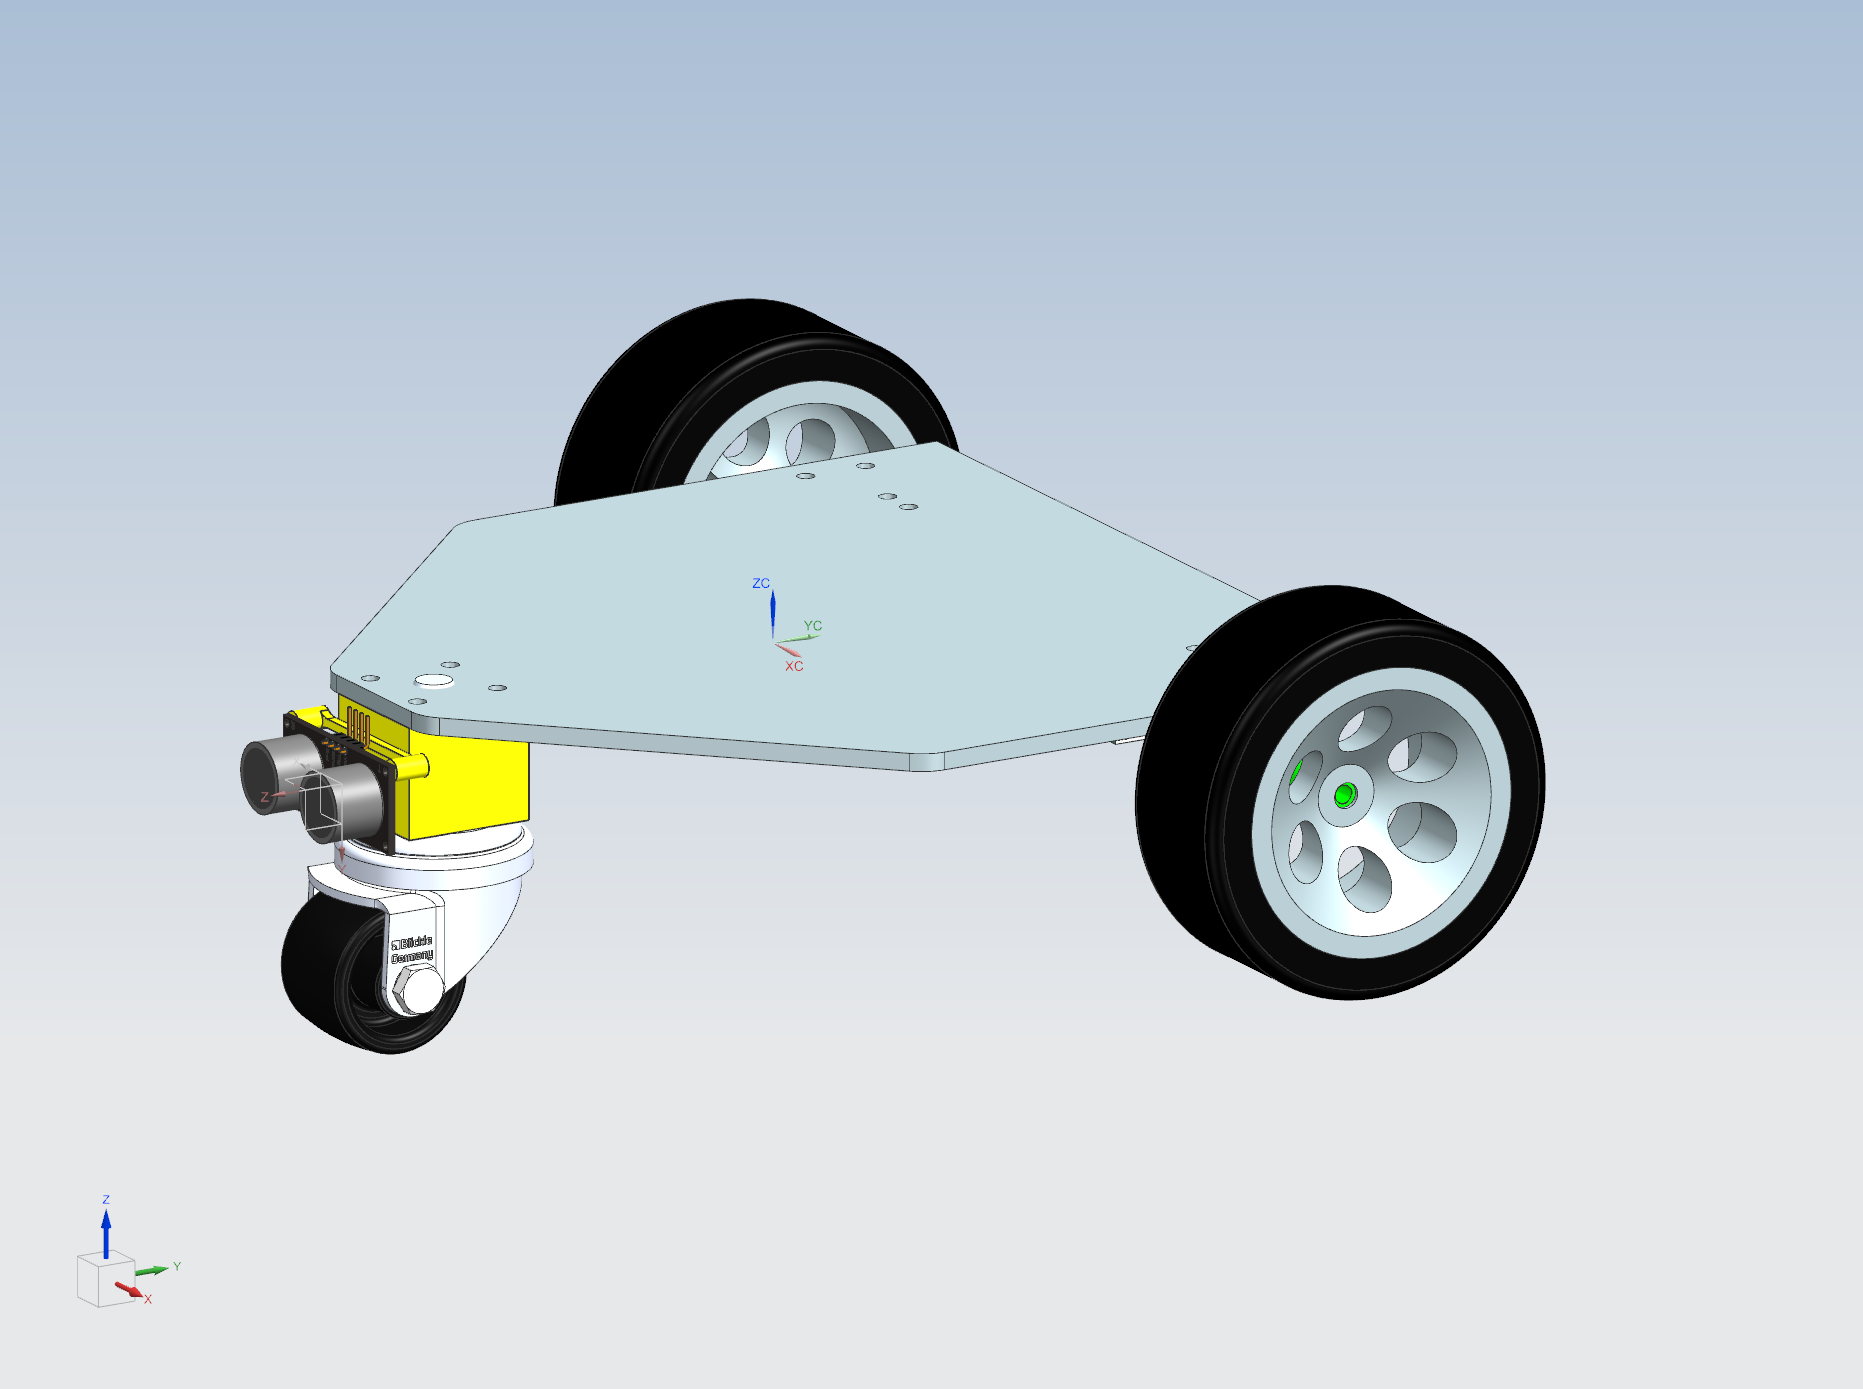
\includegraphics[width=0.9\textwidth]{assets/prototyp-fahrwerk/Prototyp_Fahrwerk_CAD.png}
\caption{Fahrwerk}
\label{fig:Prototype_Fahrwerk_CAD}
\end{figure}

Die Abbildung \ref{fig:sectionview-wheelmount} zeigt eine Schnittansicht des Antriebs. Die Räder werden mit einer Antriebswelle formschlüssig durch den Motor angetrieben. Die Welle hat radseitig ein 6-Kant angefrässt, das direkt in die Radnabe eingepasst wird und durch eine Schraube gesichert werden kann. Die Welle wird durch je ein Fest- und ein Loslager gelagert. Auf der andern Seite wird der Motor mit Hilfe des in Abbildung \ref{fig:sectionview-wheelmount} ersichtlichen Motorflansches fixiert. 

\begin{figure}[H]
\centering
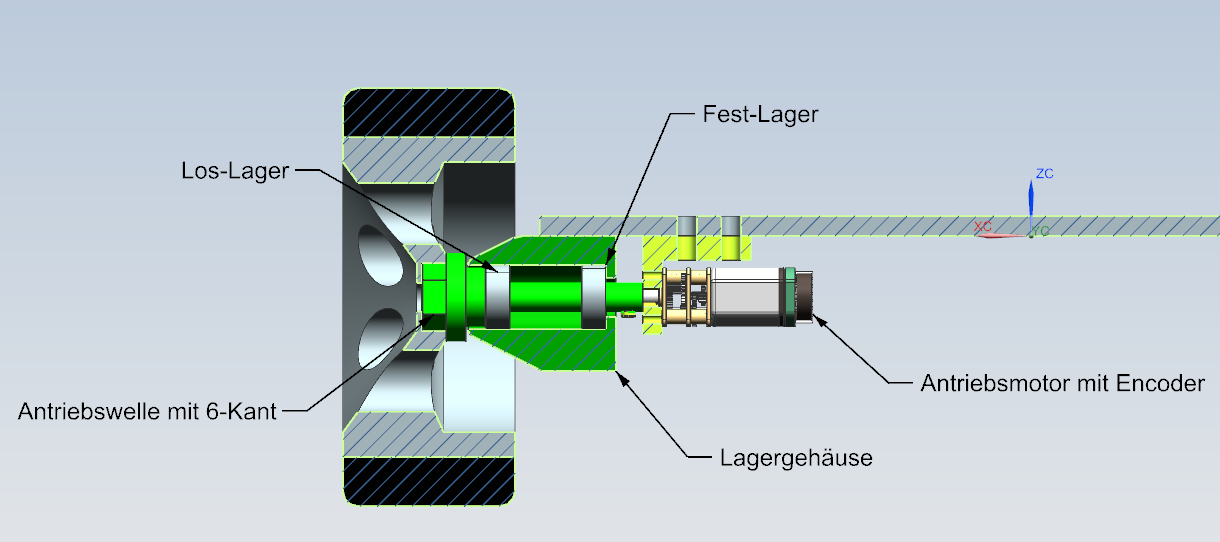
\includegraphics[width=1.0\textwidth]{img/Antrieb.png}
\caption{Schnittansicht Antrieb}
\label{fig:sectionview-wheelmount}
\end{figure}


\subsection{Linienerkennung}

Mit einem Array von Phototransistoren, Kondensatoren und Widerständen, wird die Entladezeit von Kondensatoren mittels Mikrocontroller und der Input Capture Funktion gemessen. Der Liniensensor dient als Unterstützung, damit der Roboter die Linie nicht verlässt während dem Fahren. Zusätzlich soll der Roboter bevor er losfährt, gerade vor der Linie positioniert werden, so dass er sich zumindest zu Beginn der Fahrt bereits auf der Linie befindet. Ebenfalls wird der Liniensensor gebraucht, um zu prüfen ob der Roboter auf einem Knoten steht.

\subsection{Distanzsensor}
\label{subsection:Distanzsensor}

Um die Distanz zwischen dem Roboter und einem Hindernis zu detektieren wird ein Arduino Ultraschallsensor verwendet. Der Ultraschallsensor wird sich vorne am Fahrzeug befinden, damit eine freie Sicht gewährleistet ist und keine Störungen durch das Fahrzeug selbst auftreten. Er wird, wie auf Abbildung \ref{fig:Prototype_Sensorhalter} gezeigt, oberhalb des Abstützrades montiert. Der Sensor erkennt die Distanz zum Hindernis und kann bestimmen, an welchem Punkt das Fahrzeug eine 180-Grad-Drehung durchführen muss, um sich auf den Hubvorgang vorzubereiten. Ebenfalls wird so ein Zusammenstossen mit Hindernissen verhindert, falls diese bei der Bilderkennung zuvor nicht erkannt wurden. Wird ein unerwartetes Hindernis erkannt, hält der Roboter an und macht ein Foto. Darauf soll mit Bilderkennung erkannt werden, um welche Art von Hindernis es sich handelt und was die nächsten Aktionen des Roboters sein sollen.

\begin{figure}[H]
\centering
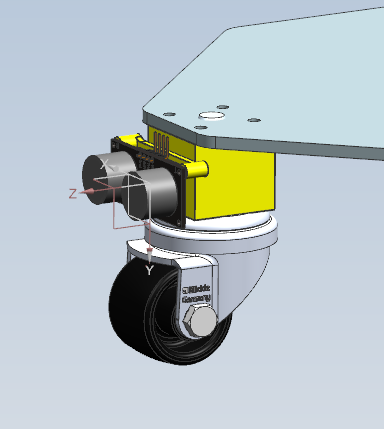
\includegraphics[width=0.5\textwidth]{assets/prototyp-fahrwerk/Prototyp_Sensorhalter.png}
\caption{Sensorhalter}
\label{fig:Prototype_Sensorhalter}
\end{figure}



\subsection{Wegfindung}

Der kürzeste Weg im Graphen vom momentanen Knoten zum Zielknoten, wird mit dem \gls{dijkstra} Algorithmus berechnet. Dieser wird zu Beginn berechnet und jedes Mal, wenn der Roboter neue Erkenntnisse zum Graph gesammelt hat, aktualisiert. 

Zusätzlich zum zukünftigen Pfad, wird der bereits befahrene Pfad gespeichert. Dies dient dazu, dass der Roboter immer in der Lage sein wird, im Fehlerzustand, auf den letzten Knoten zurück zu fahren und dabei die Orientierung behält.

\subsection{Kameraposition}

Die Kamera wird in einer Höhe von ca. 22.5cm und einem Winkel von ca. 56\textdegree\ montiert. Die Position ist fix, das heisst, es wird keine schwenkbare Kamera benötigt. In der folgenden Grafik \ref{fig:camera-position-concept} ist die Kameraposition ersichtlich. Die Kamera selbst verfügt über ein horizontales Field of View\footnote{\url{https://en.wikipedia.org/wiki/Field_of_view}} von 66\textdegree. Die Kamera wird im Hochformat verwendet. Dadurch sind im Field of View von 66\textdegree\ sowohl sehr nahe Knoten und Objekte bis zu 10cm im Bild, aber auch weit entfernte Pylonen, welche 200cm entfernt stehen.

Sowohl die Montage, als auch das Fiel of View ist in Abbildung \ref{fig:camera-position-concept} ersichtlich.

\begin{figure}[H]
    \centering
    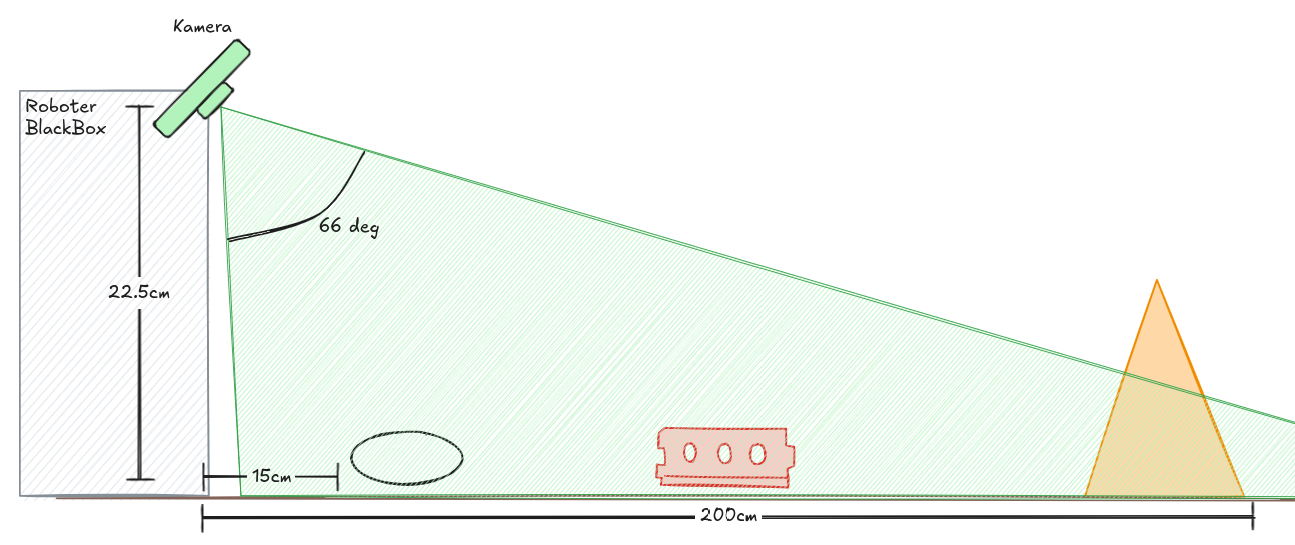
\includegraphics[width=1\linewidth]{assets//informatik-prototyp//camera/camera_position.png}
    \caption{Kamera Positionierung}
    \label{fig:camera-position-concept}
\end{figure}



\subsection{Software Steuerung}


Das Programm, welches auf das \gls{tinyk22} geladen wird, wird in C geschrieben. Mit der Entwicklungsumgebung MCUXpressoIDE kann der Code geschrieben und kompiliert werden. Das Programm kann debugged werden, da auf dem Tiny K22 ein Debugger beinhaltet ist. Es können vom Modul ``Mikrocontroller Fundamentals'' bestehende Libraries verwendet werden. Einige Anpassungen, wie zum Beispiel die \acrshort{uart}, wurden bereits vorgenommen.

\subsection{Akku}

Um das ganze System mit Spannung zu versorgen wird ein 14.8V Akku verwendet, der in einer Stunde 3000mA liefert. Daraus kann berechnet werden, dass bei einer geschätzten maximalen Leistung von 30W und einer Spannung von 12V, diese Kapazität für ca. 1.2 Stunden reicht.  

\subsection{PCB Design}

Das \acrshort{pcb} wird aus mehreren Teilen bestehen. Das Mainboard wird zentral eingebaut, da es der Knotenpunkt und der grösste \acrshort{pcb} Komponent ist. Ebenfalls wird eine separate Platine für die Spannungsversorgung benötigt, welche sich ebenfalls zentral befinden wird. Der Ultraschall- und Liniensensor befinden sich im vorderen Teil des Roboters und werden über eine Kabelverbindung mit dem Mainboard angeschlossen. Aufgrund der Wiederverwendung werden die einzelnen Komponenten, wie auch das \gls{tinyk22}, steckbar verbunden werden.

\newpage

\subsection{Schnittstellen zwischen den Kompontenten}

Im Blockschaltdiagramm in Abbildung \ref{Blockdiagramm Steuerung} wird die Hardware der Steuerung aufgezeigt. Die genauen Funktionen des Mikrocontroller sind im Prototyping Kapitel \nameref{Blockdiagramm: Schnittstellen zwischen den Komponenten} beschrieben. Im Zentrum steht der Mikrocontroller \gls{tinyk22}.
Er steuert und verarbeitet die Signale der verschiedenen Komponenten wie Motoren, Ultraschallsensor, Liniensensor oder Motortreiber. Die Verbindung zum Raspbberry Pi, der die Bilder auswertet und die Navigation implementiert, wird über \acrfull{uart} aufgebaut. Die Stromüberwachung sorgt dafür, dass keine elektrischen Komponenten durch Überlast beschädigt werden.


\begin{figure}[H]
    \centering
    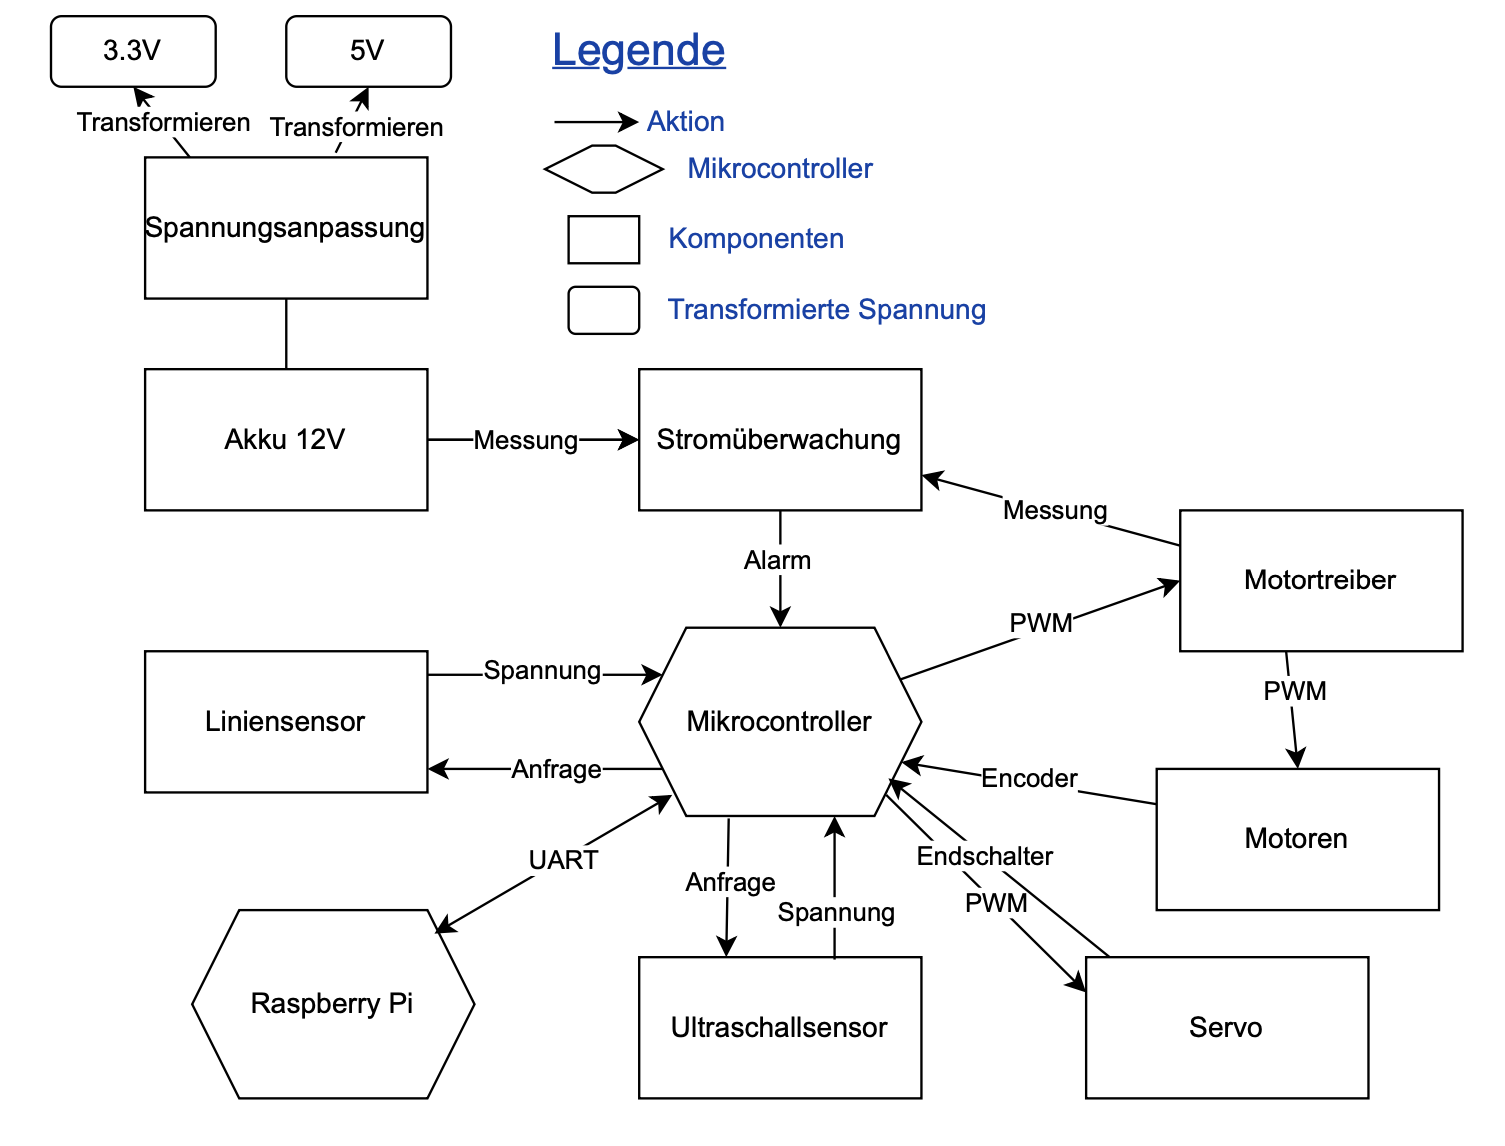
\includegraphics[width=1\linewidth]{img/Blockdiagramm-ET-drawio.drawio-2.png}
    \caption{Blockdiagramm Steuerung}
    \label{Blockdiagramm Steuerung}
\end{figure}



    \subsection{Simulator}

Das Erarbeiten des Konzeptes des Simulators, der Implementierung und des Gebrauchs wird in diesem Kapitel festgehalten.

Nach der Nutzwertanalyse war das grundlegende Konzept klar und es konnte mit der Implementierung begonnen werden.

\subsubsection{Spezifikationen}

TODO: Was soll Simulator koennen?

\begin{table}[H]
\centering
\small
\begin{tabularx}{\textwidth}{|l|X|l|}
\hline
  \textbf{Nr.} & \textbf{Spezifikation} & \textbf{Priorität 1-3}  \\
  \hline
  1  & Der Zielknoten kann ausgewählt werden. &  2\\
  \hline
   2   & Der Roboter speichert den Graph intern.  & 1\\
  \hline
   3 & Der Roboter überprüft seine Nachbarsknoten.&1\\
  \hline
  4 & Der Roboter erkennt fehlende Linien und reagiert darauf. & 1\\
  \hline
  5 &   Der Roboter erkennt Pylonen und reagiert darauf. & 1\\
  \hline
   6  &   Der Roboter erkennt Barrieren und reagiert darauf. & 1\\
  \hline
    7 &   Der Roboter berechnet den kürzesten Weg im Graphen.& 1\\
  \hline
     8  &   Der Weg des Roboters wird im GUI angezeigt. & 1\\
  \hline
      9   &   Die Reaktionen auf die Hindernisse werden im GUI angezeigt. & 2\\
  \hline
 10   &   Die Hindernisse werden im GUI angezeigt. & 2\\
  \hline
   11   &   Die Reihenfolge der Knoten wird erkannt, als Vorbereitung, dass der Roboter, der Steuerung sagen kann, wo sich der nächste Weg befindet. & 3\\
  \hline

\end{tabularx}
\caption{Spezifikationen Simulator}
\label{table:spezifikation-simulator}
\end{table}

\subsubsection{Konzeption}

Es wurden mehrere Varianten ermittelt mit einem morphologischen Kasten, die alle die Spezifikatinen erfuellen koennen. Mit einer Nutzwertanalyse wurde die beste Variante bestimmt.

TODO BEschreib gewaehlte Variante, depending wo Kasten \& Analyse sind in Doku

Die einzelnen Taetigkeiten wurden in GitHub Issues festgehalten. Jedes Issue wurde jeweils der Person zugeordnet, die gerade daran arbeitet. So konnte koordiniert entwickelt werden.

\begin{figure}[H]
\centering
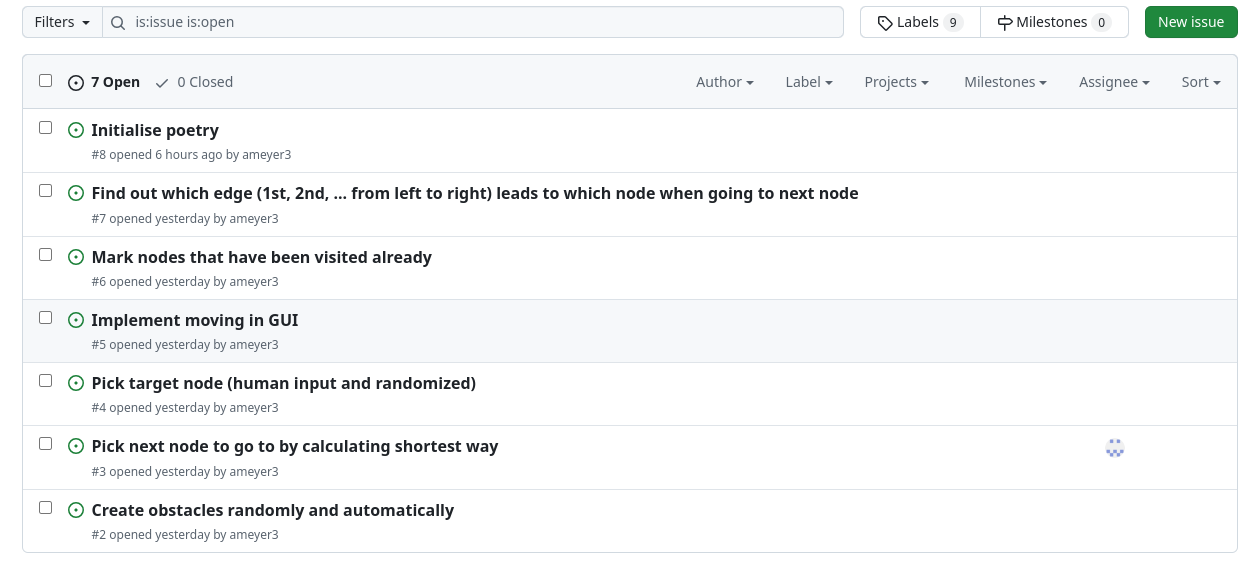
\includegraphics[width=\textwidth]{img/github-issues.png}
\caption{GitHub Issue Liste}
\label{fig:github-issues}
\end{figure}

Es wurde ein objektorientierter Ansatz gewaehlt, um den Simulator umzusetzen. Die Roboterklasse soll dabei den physischen Roboter darstellen, der die einzelnen Bauteile besitzt. So soll zum Beispiel die Wheels Klasse verwendet werden als Simulation fuer das Drehen und fortbewegen. An dieser Klasse werden diese Nachrichten gesendet, die im echten Roboter an die elektrische Steuerung gesendet werden wuerden betreffend der Fortbewegung.


\begin{figure}[H]
\centering
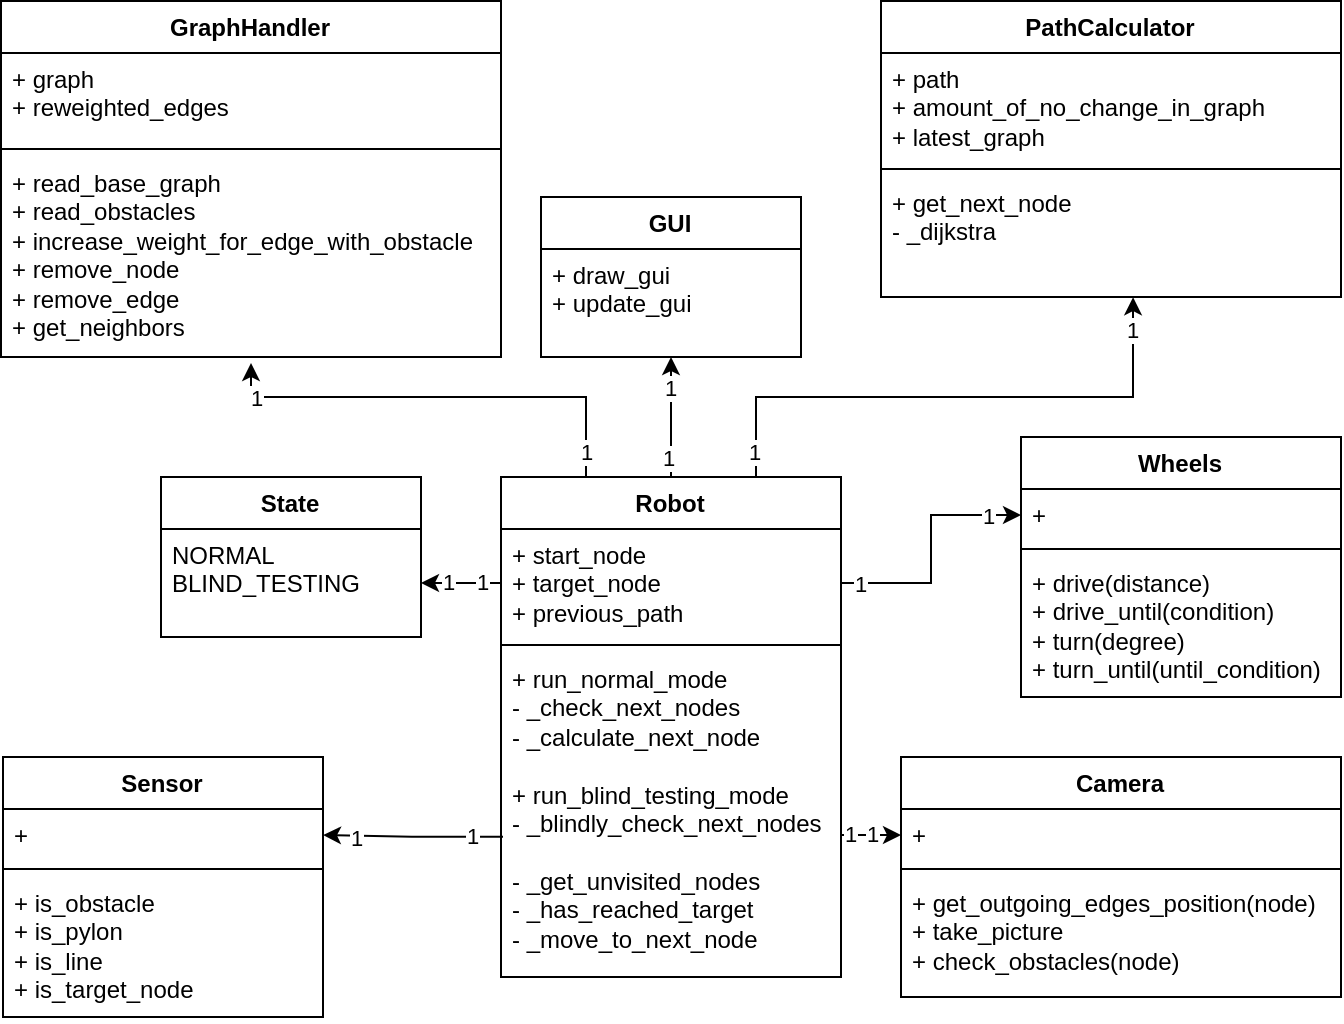
\includegraphics[width=\textwidth]{assets/informatik-prototyp/simulator/simulator-erd.png}
\caption{Simulator ERD}
\label{fig:simulator-erd}
\end{figure}

\subsubsection{Entwicklung}

Der erste Schritt war es einen Graph zu definieren. Dazu wurde ein YAML File mit dem konfigurierten Graph erstellt. 
Dazu wurde der vorgegebene Graph beschriftet: Jeder Knoten erhaelt einen Buchstaben und jede Kante ein Gewicht. Die Gewichtungen sind die relativen Laengen der Strecken. Diese Beschriftung wurde wie folgt in einem YAML File beschrieben.

\begin{figure}[H]
\begin{subfigure}{0.275\textwidth}
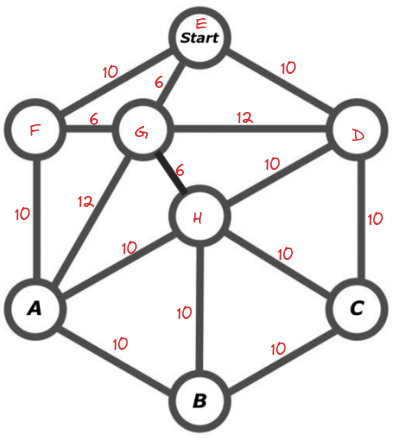
\includegraphics[width=0.95\linewidth]{img/graph_with_weighted_edges.png} 
\caption{Beschrifteter Graph}
\label{fig:labeled-graph}
\end{subfigure}
\begin{subfigure}{0.720\textwidth}
\begin{footnotesize}
\begin{verbatim}
# the edges are assorted clock-wise
A: [{ F: 10 }, { G: 12 }, { H: 10 }, { B: 10 }]
B: [{ A: 10 }, { H: 10 }, { C: 10 }]
C: [{ D: 10 }, { B: 10 }, { H: 10 }]
D: [{ E: 10 }, { C: 10 }, { H: 10 }, { G: 12 }]
E: [{ D: 10 }, { G: 6 }, { F: 10 }]
F: [{ E: 10 }, { G: 6 }, { A: 10 }]
G: [{ E: 6 }, { D: 12 }, { H: 6 }, { A: 12 }, { F: 6 }]
H: [{ G: 6 }, { D: 10 }, { C: 10 }, { B: 10 }, { A: 10 }]
\end{verbatim}
\end{footnotesize}
\caption{Graph in YAML}
\label{fig:graph-yaml}
\end{subfigure}
\end{figure}

Die Hindernisse und die fehlenden Linien sind ebenfalls in einem YAML File definiert. So koennen diese einfach angepasst werden:

\begin{verbatim}
cone:
  - F
barrier:
  - [E, G]
missing_line:
  - [E, D]
\end{verbatim}

Der Simulator liest die beiden Dateien ein und speichert sie intern als Python Dictionaries.

\textbf{Ablauf des Simulators:}

Das Ziel ist es, dass der Ablauf moeglichst nah ist an dem Ablauf des Gesamtkonzeptes.
Der Programmablauf besteht aus folgenden Teilen:
\begin{enumerate}
    \item Nachbarsknoten auf Hindernisse pruefen
    \item Naechste Knoten berechnen
    \item Zu naechstem Knoten fahren
\end{enumerate}

Es wird simuliert, dass der Roboter auf einem Knoten steht. Er dreht sich im Uhrezeigersinn im Kreis und prueft alle Nachbarsknoten. In der Simulation wird dafuer der Hindernis-Dictionary auf die jeweiligen Knoten und Strecken geprueft. Falls ein Hinderniss detektiert wirde, reagiert er wie folgt:

\begin{itemize}
    \item Ein Pylon steht auf dem Nachbarsknoten: Dieser Knoten und alle Kanten, die dahin fuehren, werden im intern gespeicherten Graph-Dictionary entfernt.
    \item Eine Barriere wird auf einer ausgehenden Strecke erkannt: Die Strecke wird im intern gespeicherten Graph-Dictionary hoeher gewichtet. TODO WIE VIEL?
    \item Eine ausgehende Linie fehlt: Diese Verbindung wird aus dem intern gespeicherten Graph entfernt.
\end{itemize}

Falls noch nie eine Berechnung des kuerzesten Weges durchgefuehrt wurde oder der intern gespeicherte Graph sich veraendert hat, wie die Berechnung der kuerzesten Pfades durchgefuehrt. Ein Dijkstra wird verwendet. Die geplante Pfad und der naechste Knoten werden gespeichert.

Danach bewegt sich der Roboter zum naechsten Knoten. Dabei wird simuliert, dass sich der Roboter zur naechsten Linie drehen soll und die Distanz zum naechsten Knoten fahren soll. Im Simulator sind alle Kanten eines Knotens im Uhrzeigersinn angeordnet gespeichert. Die Position (relativ zu der Strecke, von der der Roboter herkommt) der naechsten Strecke wird mit dem Ring Buffer Algorithmus\footnote{https://en.wikipedia.org/wiki/Circular\_buffer} berechnet. So kann Simuliert werden, dass eine Liste in einem Kreis angeordnet ist. So wird es in der richtigen Applikation moeglich sein, die Kanten zu identifizieren. 

\begin{figure}[H]
\centering
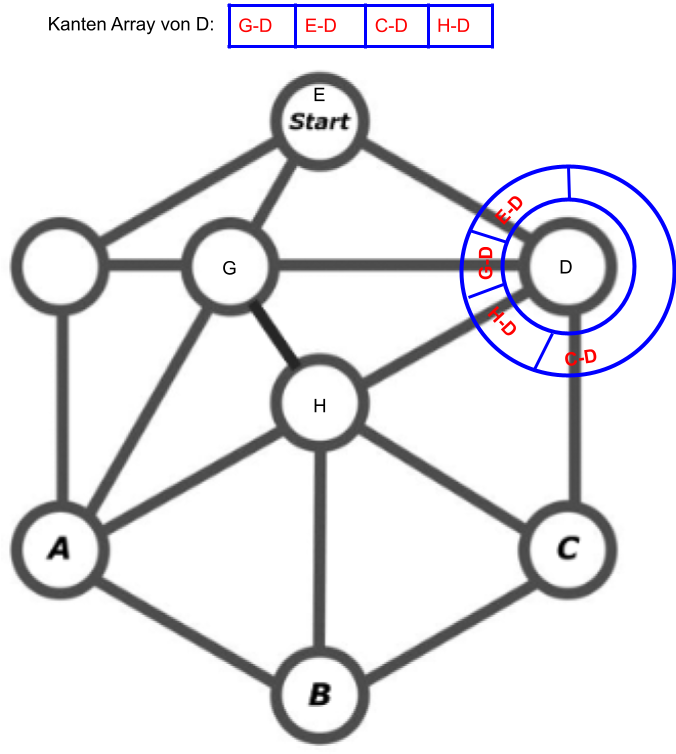
\includegraphics[width=0.75\textwidth]{assets/informatik-prototyp/simulator/ring-buffer-graph.png}
\caption{Graph with Ring Buffer}
\label{fig:ring-buffer-graph}
\end{figure}

Die Position relativ zu einer bestimmten Kante herauszufinden wird wie folgt implementiert:

\begin{verbatim}
edges_to_target = (target_index - start_index) % len(neighbors)
\end{verbatim}

Diese Ablauf wird so lange wiederholt, bis der Zielknoten erreicht wird.
Waehrend des ganzen Ablaufes werden die einzelnen Klassen aufgerufen, die die einzelnen Roboterbauteile simulieren. In diesen befindet sich zum Teil eine Mock-Logik (zum Beispiel Hindernisse aus dem Konfigurationsfile lesen anstatt aus Bildern von der Kamera) und oft nur simple Print Statements. Diese Print Statements sollen die Schnittstelle zu der Elektronik simulieren. Ein Beispiel davon ist die Wheels Klasse:

\begin{verbatim}
class Wheels:
    def drive(self, distance: int):
        print(f"DRIVE {distance}CM.")

    def turn(self, degree: int):
        print(f"TURN {degree} DEGREES.")

    # Turns until sensor detect objects
    def turn_until(self, until_condition: str):
        print(f"TURN {until_condition}.")
        is_line = False
        while not is_line:
            print("Turning")
            # Simulate that a line was detected by a sensor
            is_line = True
        print(f"Found the next line to traverse.")
\end{verbatim}

\textbf{Reset}

TODO
Falls etwas erkannt mit Sensoren, dass nicht erkannt wurde mit Kameras, zuruecksetzen und das was getroffen wurde in Graph intern eintragen

\textbf{Technische Aspekte:}

Um die Abhaengigkeiten zu externen Bibliotheken zu organisieren wird Poetry\footnote{https://python-poetry.org/} verwendet. Dabei werden die Bibliotheken in eine virtuelle Umgebung installiert, worin der Simulator ausgefuehrt wird.

\textbf{Graphical User Interface:}

Das GUI wurde mit PyGame\footnote{https://www.pygame.org/news} umgesetzt. Der Graph wird mit beschrifteten Knoten dargestellt. Der Roboter ist ein Kreis mit einem Dreieck. Die Spitze des Dreiecks zeigt die Richtung, in welche der Roboter schaut.
Der Fahrt des Roboters auf den Linien ist ebenfalls dargestellt.

Auf folgendem Bild dreht sich unser Roboter auf der Stelle im Kreis, um die umliegenden Knoten und Kanten zu ueberpruefen.
Das orangene Dreieck stellt einen Pylon dar, das rote Rechteck ein Hindernis, das beseitigt werden kann und das rote Kreuz ist eine Linie, die fehlt. Die rote Fahne ist das Ziel, das der Roboter erreichen soll.

\begin{figure}[H]
\centering
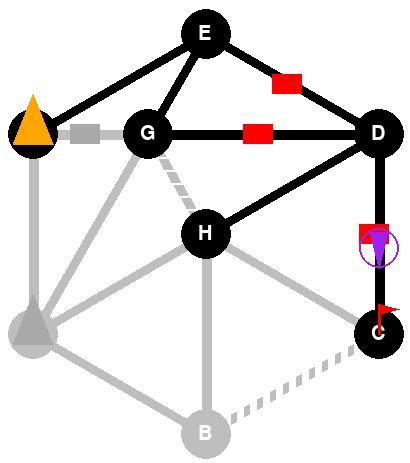
\includegraphics[width=0.75\textwidth]{assets/informatik-prototyp/simulator/sim-ui.png}
\caption{GUI des Simulators}
\label{fig:sim-gui}
\end{figure}

TODO BILD: Roboter auf Kante, mit entfernten Kanten 

\textbf{Trial and Error Mode}

Es wurde ein Modus implementiert, zu dem gewechselt wird, falls der Roboter nicht mehr weiss, wo er sich befindet. Dies soll im richtigen Roboter als Risikomitigation implementiert sein. Fuer die Simulation wurde ein Ablauf definiert fuer diesen Modus und er wurde implementiert. Die Nachrichten der Sensoren wurden gemockt.

\begin{figure}[H]
\centering
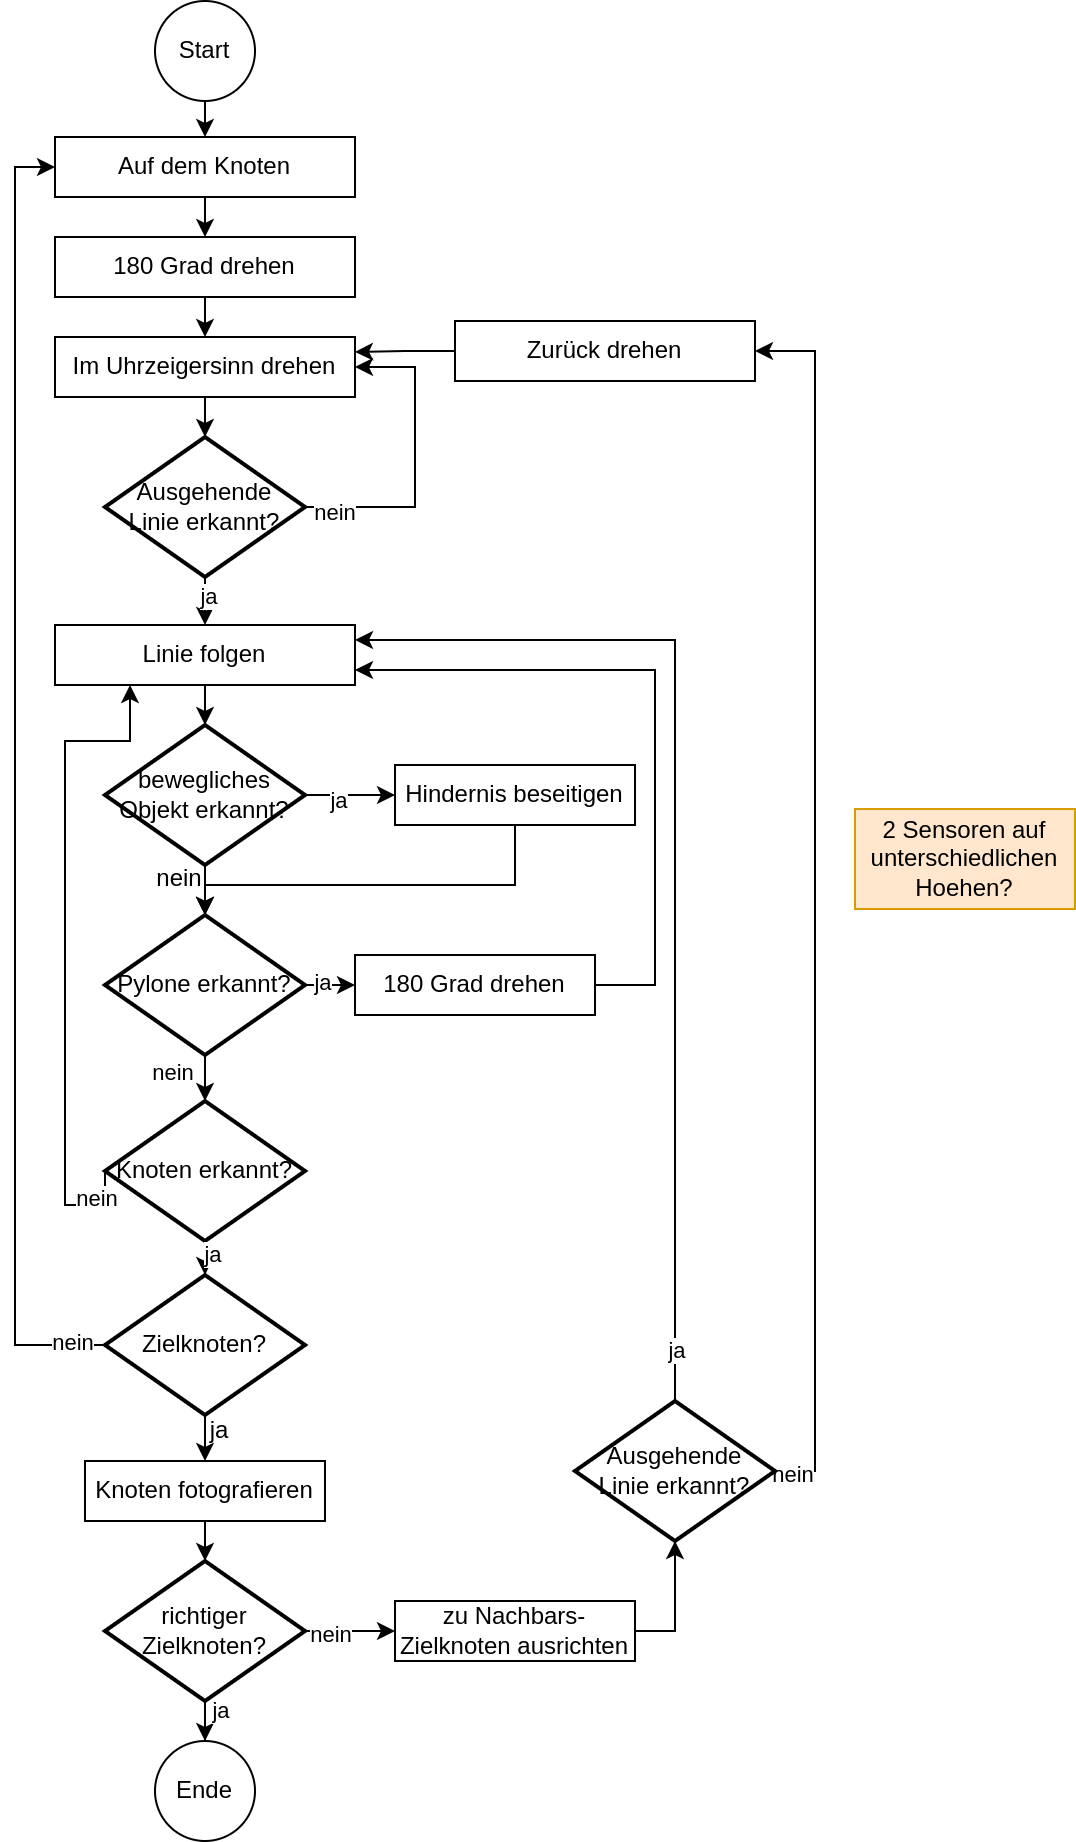
\includegraphics[width=0.75\textwidth]{assets/informatik-prototyp/simulator/simulator-trial-and-error-mode.png}
\caption{Trial and Error Mode}
\label{fig:sim-trial-error}
\end{figure}


    \section{Nachhaltigkeit}
\label{section:Nachhaltigkeit}

Das Thema der Nachhaltigkeit wird zurecht immer relevanter und wurde aus diesem Grund in diesem Projekt berücksichtigt. In den folgenden Kapiteln wird aufgezeigt auf welche Arten nachhaltig gearbeitet wurde.

%%%%%%%%%%%%%%% MT NACHHALTIGKEIT %%%%%%%%%%%%%%%%%%%%%
%%%%%%%%%%%%%%%%%%%%%%%%%%%%%%%%%%%%%%%%%%%%%%%%%%%%%%%

MT NACHHALTIGKEIT IN PROGRESS

%%%%%%%%%%%%%%% ET NACHHALTIGKEIT %%%%%%%%%%%%%%%%%%%%%
%%%%%%%%%%%%%%%%%%%%%%%%%%%%%%%%%%%%%%%%%%%%%%%%%%%%%%%

\subsection{Motorentest}

Der Motorentest wurde im Labor der Hochschule durchgeführt. Für den Aufbau wurde ein Steckplatine verwendet, diese kann mehrmals genutzt werden. Die nötigen elektronischen Bauteile wurden nicht extra bestellt, sondern von der Werkstatt ausgeliehen. Um den Stromverbrauch gering zu halten wurde der Motor zwischen den Tests ständig abgeschaltet. 

\subsection{Leiterplatten}
\label{Leiterplatten}

Leiterplatten oder auch \acrfull{pcb} sind aus der modernen Elektronik nicht mehr wegzudenken. Allerdings sind mit der aktuellen Technologie einige Herausforderungen verbunden. Viele der verwendeten Materialien, wie beispielsweise Blei, sind giftig für die Umwelt. Andere, wie der in der Fertigung eingesetzte Klebstoff, sind nicht biologisch abbaubar.

Die Minimierung von Abfall beginnt bereits bei der Planung und dem Design der Schaltung. Für die Produktion von einmaligen Prototypen sollten Designansätze gewählt werden, die eine Weiterverwendung der Bauteile nach Abschluss des Projekts ermöglichen, anstatt sie zu entsorgen. Komplexe Formen und Aussparungen in den Leiterplatten führen zu erhöhtem Materialabfall und sollten ebenfalls vermieden werden.

Es gibt bereits die Möglichkeit, sogenannte „grüne“ \acrshort{pcb}'s herzustellen, die aus umweltfreundlicheren Materialien gefertigt werden\footnote{https://de.venture-mfg.com/Was-sind-biologisch-abbaubare-Leiterplatten\%3F/}.  Derzeit sind diese jedoch noch kostenintensiv und werden im Rahmen dieses Projekts nicht berücksichtigt.

\subsection{Wiederverwendbarkeit}

Wie im Kapitel Leiterplatten \ref{Leiterplatten} beschrieben, hat die Wiederverwendbarkeit einzelner Komponenten einen positiven Einfluss auf die Nachhaltigkeit. Aus diesem Grund wird nicht eine grosse, monolithische Leiterplatte entwickelt, sondern mehrere kleinere Platinen, die jeweils auf spezifische Teilaufgaben abgestimmt sind.

Ein Beispiel dafür ist die Verwendung eines separaten Moduls für den Mikroprozessor, wie etwa beim Modell \acrfull{tinyk22} \ref{fig:Tiny_K22_PCB}. Dieses modulare Design ermöglicht es, einzelne Komponenten dieses Projekts auch in zukünftigen Vorhaben weiterzuverwenden, wodurch Materialressourcen effizienter genutzt und Abfälle reduziert werden können.

\subsection{Transport}

Ein Grossteil der Elektronikkomponenten wird aus China oder Taiwan importiert. Die damit verbundenen Transportwege, sei es per Flugzeug oder Schiff, sind in der Elektronikindustrie allgegenwärtig.

Für die Herstellung eines einzelnen Prototyps ist der Aufbau einer eigenen Industrie zur Produktion in der Schweiz wirtschaftlich nicht sinnvoll. Ebenso wurde in diesem Projekt keine Zeit darauf verwendet, alternative Bezugsquellen bei europäischen Herstellern zu identifizieren und einzubeziehen.

\subsection{Energie}

Die Herstellung der einzelnen Elektronikkomponenten erfordert erhebliche Mengen an Energie. Da die Energieproduktion zu den grössten Verursachern von Umweltbelastungen gehört, ist es sinnvoll, den Energiemix der Hauptproduktionsstandorte zu berücksichtigen.

Die Bauteile für dieses Projekt stammen überwiegend aus den USA, China\footnote{https://www.bpb.de/kurz-knapp/zahlen-und-fakten/europa/75143/eu-usa-china-energiemix/} und Taiwan\footnote{https://moeaea.gov.tw/ECW/English/content/Content.aspx?menu_id=1679}, während die Endmontage in der Schweiz erfolgt. In den Produktionsländern USA, China und Taiwan wird ein Grossteil der Energie aus fossilen Brennstoffen wie Kohle gewonnen, was erhebliche CO$_{2}$-Emissionen verursacht. Obwohl diese Form der Energiegewinnung umweltschädlich ist, stellt sie in der globalen Lieferkette eine gegenwärtige Realität dar, die sich kurzfristig nicht ändern lässt. Diese Länder bieten aufgrund ihrer etablierten Produktionsinfrastruktur und ihrer Kosteneffizienz wesentliche Vorteile, die sie zu unverzichtbaren Akteuren in der Elektronikfertigung machen.

Im Gegensatz dazu erzeugt die Schweiz ihren Strom überwiegend aus erneuerbaren Quellen\footnote{https://www.kernenergie.ch/de/schweizer-strommix-_content---1--1069.html}, insbesondere aus Wasserkraft, wodurch die Endmontage mit einem deutlich geringeren CO$_{2}$-Ausstoss verbunden ist. Die Menge an CO$_{2}$, die durch die Energieversorgung der einzelnen Komponenten freigesetzt wurde, wird in diesem Projekt jedoch nicht untersucht.



%%%%%%%%%%%%%%% IT NACHHALTIGKEIT %%%%%%%%%%%%%%%%%%%%%
%%%%%%%%%%%%%%%%%%%%%%%%%%%%%%%%%%%%%%%%%%%%%%%%%%%%%%%

\subsection{Bilderkennung}

Die Bilder wurden bereits früh mit einem Raspberry Pi und eine Raspberry Pi Kamera aufgenommen. Bevor dafür etwas neues bestellt wurde, wurden ein Raspberry Board und eine Kamera verwendet, die ein Teammitglied bereits zu Hause hatte. Beide hatten ebenfalls je eine Hülle.
Um die beiden Einzelteile miteinander zu verwenden, wurden sie lediglich zusammengeklebt, damit nicht eine neue Hülle gedruckt oder gekauft werden muss, die wahrscheinlich nicht im Roboter verwendet werden wird.
Um die Höhe und die Ausrichtung der Kamera zu simulieren, wurde ein kleines Stativ verwendet, das ebenfalls schon im Besitz eines Teammitgliedes war.
Erst nachdem klar war, dass die Qualität der Bilder in Ordnung ist, wurden die neusten Versionen der Raspberry Pis, die mehr Rechenleistung liefern, bestellt. Die Bestellung wurde über die schweizer Seite Digitec getätigt und die Hardware war bereits im lokalen Lager von Digitec. 

\subsection{Code Repositories}

Die Code Repositories befinden sich auf GitHub. Dabei gibt es für den Simulator keine GitHub Action\footnote{https://docs.github.com/en/actions/about-github-actions/understanding-github-actions}, die den Code testet. Dies bedeutet, dass nur das Minimum an Rechenleistung von den GitHub Server verwendet wird, sprich, nur diesen Speicher, der nötig ist, um Code zu speichern. Die automatischen Tests werden lokal ausgeführt.

Zusätzlich setzt sich GitHub für Nachhaltigkeit ein.\cite{github-sustainability}

Sie haben mit drei anderen Firmen die Green Software Initiative gegründet. Diese soll dabei helfen grüne Software zu erstellen.  Dabei geht es um Software Tools, die sich ihrem Kohlenstoffausstoss bewusst sind und dabei effizient handeln. Das Ziel von der Green Software Initiative ist es, Kohlenstoff zu reduzieren und nicht nur zu neutralisieren.\cite{green-software-initiative}

GitHub hat ebenfalls bei One Tree Planted mitgemacht. Deren Ziel ist es, die Umwelt wieder herzustellen, indem Bäume gepflanzt werden\cite{one-tree-planted}. Auch mit The Ocean Cleanup hat GitHub kollaboriert. Diese wollen Plastik aus den Meeren entfernen.\cite{ocean-cleanup}.

Ausserdem wird nachhaltige Software von GitHub unterstützt und gefördert. So gibt es ein GitHub Repository, dass eine extensive Liste von grüner Software hat. Sie sind in 4 Kategorien eingeteilt: Messungssoftware, Kohlenstoffeffizienz, Kohlenstoffbewusstsein und spezielle Tools. Dieses Repository wird von GitHub selber gefördert.\cite{green-software}

GitHub ist seit 2019 CO2-neutral und hat auch weitere nachhaltige Ziele. 2025 soll GitHub zu 100\% auf erneuerbare Energien setzen und in 2030 sogar CO2-negativ sein.\cite{github-goals}





%%%%%%%%%%%%%%% ALLG NACHHALTIGKEIT %%%%%%%%%%%%%%%%%%%
%%%%%%%%%%%%%%%%%%%%%%%%%%%%%%%%%%%%%%%%%%%%%%%%%%%%%%%


\subsection{Dokumentation}

Damit Overleaf produktiv für unsere LaTeX Dokumentation verwendet werden konnte, wurde eine Vollversion benötigt. Damit das Budget nicht dafür verwendet werden musste, wurde eine eigene Overleaf Instanz aufgesetzt. Damit diese möglichst nachhaltig läuft, wurde sie auf einem Server aufgesetzt, der einen anderen Hauptzweck hat und bereits vor PREN immer eingeschaltet war. So wird kein zusätzlicher Strom benötigt.

Das Backup der Dokumentation ist auf einem anderen Server eingerichtet. Auch dieser Server lief bereits vorher Non-Stop und hat eigentlich einen anderen Zweck. Zusätzlich wird das Backup auf einmal am Tag beschränkt, damit nicht bei jeder Änderung ein Backup gestartet wird. Das Backup wird auf GitHub gepusht und in einer GitHub Action wird die LaTeX Dokumentation zu einem PDF gebaut. Dadurch, dass dies maximal einmal am Tag geschieht, wird die Nutzung des geteilten Speichers von GitHub gesenkt.

\subsection{Datenaustausch}

Zu Beginn des Projektes wurde in der Gruppe entschieden, dass auf jegliches Papier verzichtet wird. Der gesamte Datenaustausch findet elektronisch statt. Es wird komplett auf Flipcharts oder Notizpapier verzichtet. Alle Mitglieder besitzen ein elektronisches Tablet, welches Papier sehr einfach ersetzen kann.
    
    \section{Projektmanagement}

Die Vorgehensweise orientiert sich an Scrum, wird jedoch angepasst auf dieses Projekt.
Scrum ist eine agile, inkrementelle Projektentwicklungsmethode, die oft in der Softwareentwicklung verwendet wird. Dabei wird in Zeitboxen, die Sprint genannt werden, gearbeitet. Pro Sprint gibt es mehrere Tasks, die bearbeitet werden sollen, sowie Sprintziele. Dies wird in diesem Projekt so gemacht.\cite{wikipedia-scrum}

Normalerweise gibt es tägliche Synchronisationsmeetings. Im Rahmen dieses Projektes werden diese wöchentlich durchgeführt, ansonsten wird eher asynchron gearbeitet.

Die Besprechungen der Testatabgaben mit dem Coach dienen als Sprintreviews. Retrospektiven werden nicht strukturiert durchgeführt, jedoch wird zu Ende jedes Sprints besprochen, ob die Arbeitsweise angepasst werden soll für den nächsten Sprint.

Als Scrum Board wird Microsoft Teams verwendet. Der Backlog wird zu Beginn der Projektes definiert und in einzelne Sprintbacklogs aufgeteilt.

\subsection{Projektorganisation}

Da es sich um eine interdisziplinarische Produktentwicklung handelt, wurde das Team aus jeweils zwei Studierenden aus den Studiengängen Elektrotechnik, Informatik und Maschinentechnik zusammengeführt. In Abbildung \ref{fig:Organigramm} ist die Projektorganisation ersichtlich. 

Im Team wurde Alina Meyer als Projektleiterin gewählt. Zudem benötigt es für die mechanischen und elektrischen Werkstätten in der Hochschule Luzern jeweils eine zuständige Person im Team. Diese wurden Ivan Zimmerman (\acrshort{elektrotechnik}) und Elias von Atzigen (\acrshort{maschinentechnik}) zugeteilt.

Die klare Aufteilung der Rollen ermöglicht es dem Team effizient und zielgerichtet an der Entwicklung des Projekts zu arbeiten. Durch diese Struktur wird gewährleistet, dass jede technische Disziplin angemessen abgedeckt ist und die Kommunikation innerhalb des Teams reibungslos funktioniert.

\begin{figure}[H]
\centering
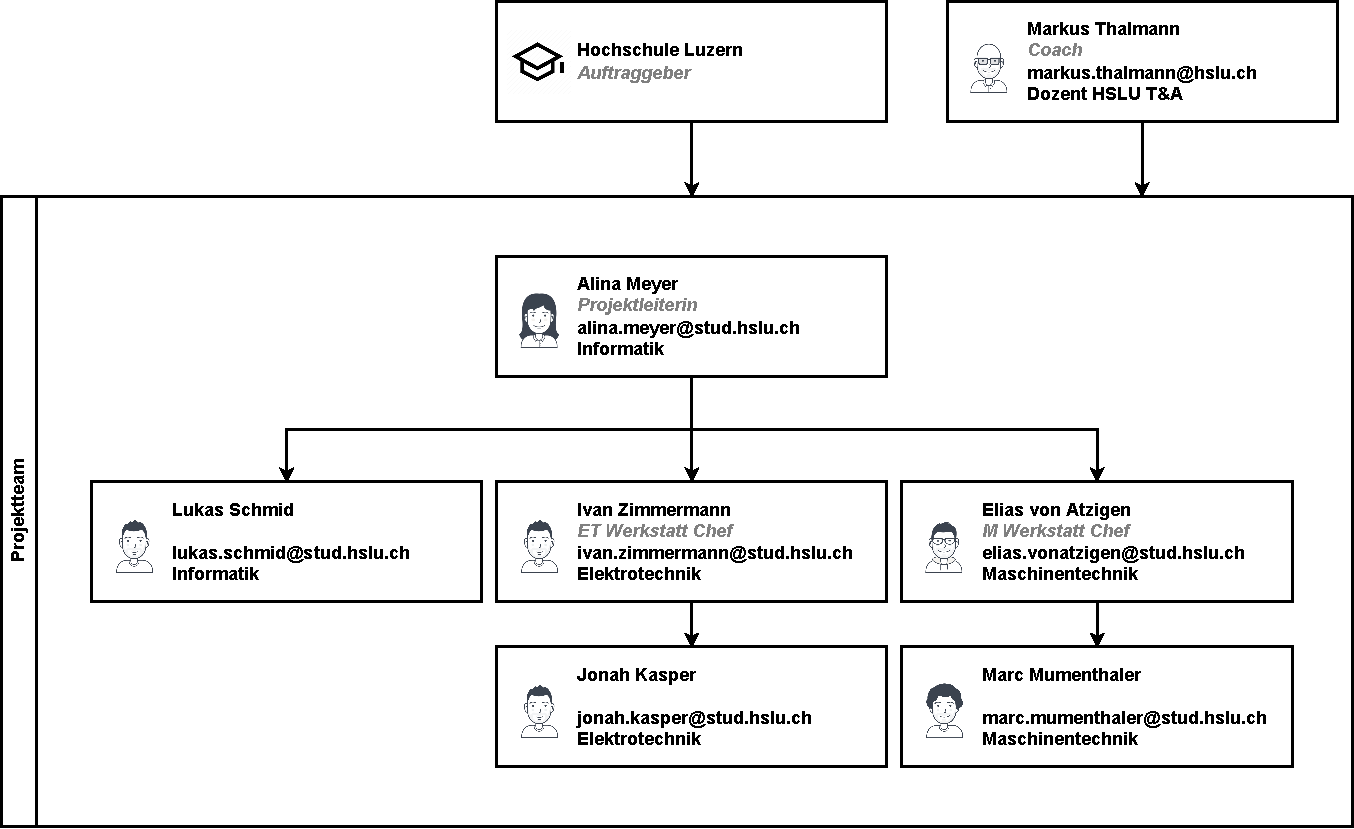
\includegraphics[width=\textwidth]{img/Projektorganisation.pdf}
\caption{Organigramm}
\label{fig:Organigramm}
\end{figure}

\subsection{Datenaustausch}

Zur Zusammenarbeit in diesem Projekt wurde ein Team auf Microsoft Teams erstellt.
Darin ist eine Datenablage, ein Taskboard und ein Chat enthalten. Der Chat wird jedoch weniger verwendet, da die Kommunikation hauptsächlich über WhatsApp erfolgt, damit die Antwortzeiten möglichst kurz sind.

Auf der folgenden Grafik \ref{fig:scrum-board} ist das Scrum Board in Teams ersichtlich. Ebenfalls sind in den Tabs auch die Dateiablage und der Chat sichtbar.

\begin{figure}[H]
\centering
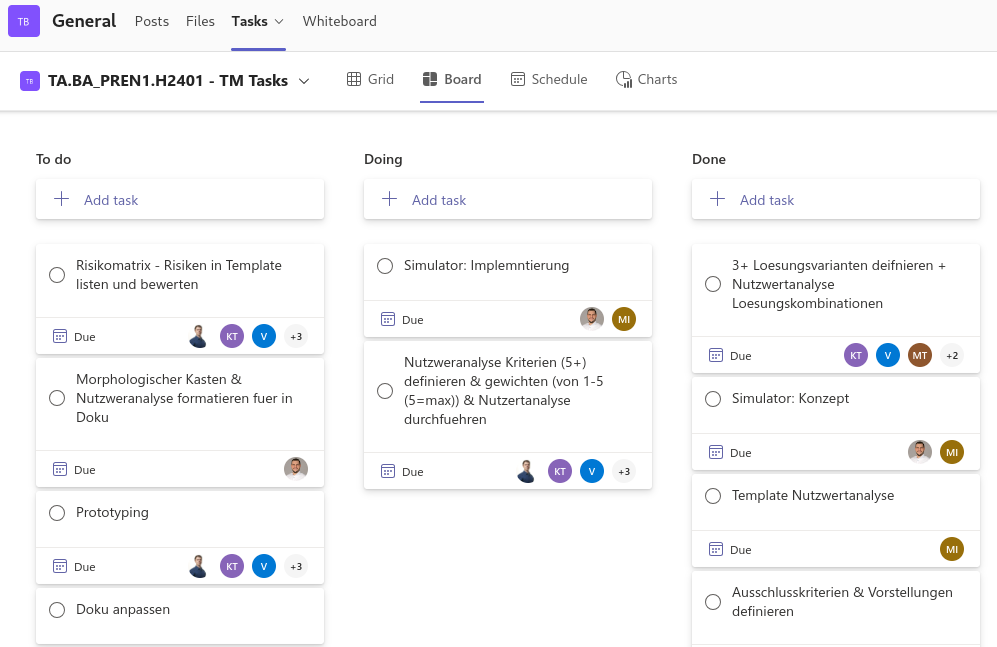
\includegraphics[width=\textwidth]{img/scrum-board.png}
\caption{Scrum Board}
\label{fig:scrum-board}
\end{figure}

Die Dokumentation wird auf einer eigenen Overleaf Instanz in LaTeX erstellt.

Eine detaillierte Auflistung des Datenaustausches und aller Kommunikationsschnittstellen befindet sich im Anhang im Kapitel \ref{kommunikationsplan} Kommunikationsplan.

Der erstellte Code wird auf GitHub gespeichert. Die Planung für den Simulator wird ebenfalls auf GitHub durchgeführt mithilfe von Issues.


    \section{Projektplanung}

Die Projektplanung wurde anhand der vorgegebenen Abgabetermine durchgeführt.
Da es vier Abgabetermine gibt, wurde das Projekt in vier Sprints aufgeteilt, die jeweils mit einem Meilenstein enden.

\subsection{Risikobewertung}

Die Risiken des Projektes sind gesammelt und bewertet worden das Resultat davon kann der folgenden Grafik entnommen werden.

BILD

Mithilfe von Prototypen sollen so viele Risiken wie möglich, so gut wie möglich vermindert werden. Zum einen wird nach Möglichkeiten gesucht, um das Eintreten zu verhindern, sowie den Schaden bei einem Eintreten zu verkleinern.

\subsection{Projektplan}

Der Projektplan in Tabelle \ref{table:projektplan} zeigt die Meilensteine, die zu erreichen sind.
Die Meilensteine sind die einzelnen Testatabgaben.
Die abzugebenden Dokumente pro Testat bilden die einzelnen Sprintziele.

\begin{table}[h!]
\centering
\begin{tabular}{|l  l l|}
\hline
  \textbf{Meilenstein} & \textbf{Datum} & \textbf{Beschreibung} \\
  \hline
  Meilenstein 1  & 04. Oktober 2024 & \makecell{Projektplan, Skizzierung der Aufgabenstellung,\\ Technologierecherche, Anforderungsliste}\\
  \hline
  Meilenstein 2  & 01. November 2024 & \makecell{Evaluation der Lösungsprinzipien, Auswahl der\\ optimalen Lösungeskombinationen}\\
  \hline
  Meilenstein 3  & 06. Dezember 2024 & \makecell{Freigabe des Gesamtkonzepts, Simulator Wegplanung, \\Dokumentation zu 80\% fertiggstellt}\\
  \hline
  Meilenstein 4  & 10. Januar 2025 & \makecell{Schlussbereicht, Präsentation}\\
  \hline
\end{tabular}
\caption{Projektplan}
\label{table:projektplan}
\end{table}

\subsection{Backlog}

Der Backlog dient als zentrales Planungselement.
In diesem Projekt sind die einzelnen Meilensteine vorgegeben. Aus diesem Grund wurden bereits zu Beginn alle Sprints geplant und der ganze Product Backlog wurde in Sprintbacklogs aufgeteilt. Nach Erreichen eines Meilensteins wird ein Ausblick auf den nächsten Sprint durchgeführt, um allfällige Anpassungen an dem Sprintbacklog vorzunehmen.

\subsection{Sprintplanung}

In den folgenden Kapiteln wurden für jeden Sprint Sprintziele definiert und ein Sprintbacklog erstellt. Für den Sprintbacklog wurden die einzelnen Meilensteine aus dem Projektplan in Epics\footnote{https://www.atlassian.com/agile/project-management/epics} beschrieben. Zu den Epics wurden User Stories erstellt. Der Aufwand der einzelnen Stories wurde mit T-Shirt Grössen geschätzt. Die einzelnen T-Shirt Grössen werden wie folgt in eine Zeitdauer umgerechnet:

\begin{table}[h!]
\centering
\begin{tabularx}\textwidth{|X | X |}
\hline
  \textbf{Grösse} & \textbf{Dauer} \\
  \hline
  S  & 4h - 2d \\
  \hline
  M  & 2d - 5d\\
  \hline
  L  & 5d+\\
  \hline
\end{tabularx}
\caption{T-Shirt Grössen}
\label{table:t-shirt}
\end{table}


\newpage
\subsubsection{Sprint 1: 20. September 2024 - 04. Oktober 2024}

\textbf{Sprintziel:}
\begin{itemize}
    \item Projektplan erstellt
    \item Aufgabenstellung skizziert
    \item Andorderungsliste erstellt
    \item Technologierecherche
\end{itemize}

\textbf{Sprintbacklog:} Der Sprintbacklog von Sprint 1 ist in Tabelle \ref{table:sprint1-backlog} dargestellt.

\begin{table}[H]
\centering
\small
\begin{tabularx}{\textwidth}{|l|l|X|c|}
\hline
  \textbf{Nr.} & \textbf{Titel} & \textbf{Beschreibung} & \textbf{Size}\\
  \hline
  1  & \textbf{Projektorganisation definieren} &&\\
  \hline
  1.1  & Rollendefinition & Die Rollen Projektleiter und Werkstattverwantwortliche werden definiert. & S\\
  \hline
  1.2 & Datenaustausch definieren & Zentrale Datenablage und Kommunikationsschnittstellen definieren.& S\\
  \hline
  1.3 & Ziele definieren & Definieren, wie wir uns den Roboter vorstellen. & S\\
  \hline
  1.4 & Vorgehen definieren & Geeignete Projektmethode wird gewählt. & S\\
  \hline
  2 & \textbf{Aufgabenstellung klären} && \\
  \hline
  2.1 & Anforderungsliste erstellen & Anforderungen, die der Roboter erfüllen muss sammeln& M \\
  \hline
  2.2 & Aufgabenstellung skizzieren & Modellierunge der Aufgabe zum Verständnis. & S \\
  \hline
  3 & \textbf{Projektplanung} && \\
  \hline
  3.1 & Projektplan erstellen & Meilensteine definieren. & S \\
  \hline
  3.2 & Backlog erstellen & Product Backlog für alle Sprints erstellen. & M \\
  \hline
  4 & \textbf{Lösungsvarianten erarbeiten} && \\
  \hline
  4.1 & Teilfunktionen finden & Roboter in Teilfunktionen aufteilen & S \\
  \hline
  4.2 & Technologierecherche & Recherche zu den einzelnen Teilfunktionen  durchführen. & L\\
  \hline
 
\end{tabularx}
\caption{Sprint 1 Backlog}
\label{table:sprint1-backlog}
\end{table}

\newpage
\subsubsection{Sprint 2: 04. Oktober 2024 - 01. November 2024}

\textbf{Sprintziel:}
\begin{itemize}
    \item Evaluation der Lösungsprinzipien
    \item Auswahl der optimalen Lösungeskombinationen
\end{itemize}

\textbf{Sprintbacklog:} Der Sprintbacklog von Sprint 2 ist in Tabelle \ref{table:sprint2-backlog} dargestellt.


\begin{table}[H]
\centering
\small
\begin{tabularx}{\textwidth}{|l|l|X|c|}
\hline
  \textbf{Nr.} & \textbf{Titel} & \textbf{Beschreibung} & \textbf{Size}\\
  \hline
  1  & \textbf{Evaluation Lösungsvarianten} &&\\
  \hline
  1.1  & Workshop Auschlusskriterien & Brainstorming, um herauszufinden, was wir nicht wollen, um Technologien auszuschliessen. & S\\
  \hline
  1.2 & Erste Aussortierung & Lösungsvarianten aussortieren ahhand Auschlusskriterien. & M\\
  \hline
  1.3 & Morphologischer Kasten & Morphologischer Kasten erstellen, um Lösungskombinationen zu ermitteln. & L\\
  \hline
  1.4 & Nutzwertanalyse & Nutzwertanalyse durchführen, um passendste Lösungskombinationen zu ermitteln. & L\\
  \hline
  2 & \textbf{Simulator} && \\
  \hline
  2.1 & Entwicklungsumgebung & Entwicklungsumgebung erstellen. & S \\
  \hline
  2.2 & Konzept erarbeiten & Konzept des Simulators definieren analog zu der Evaluation der anderen Lösungsvarianten. & M \\
  \hline
  2.3 & Wegfindung implementieren & Wegfindung in einem Graphen implementieren. & M \\
  \hline

\end{tabularx}
\caption{Sprint 2 Backlog}
\label{table:sprint2-backlog}
\end{table}

\newpage
\subsubsection{Sprint 3: 01. November 2024 - 06. Dezember 2024}

\textbf{Sprintziel:}
\begin{itemize}
    \item Dokumentation ist zu 80\% fertiggestellt
    \item Simulator ist fertiggstellt
    \item Freigabe des Gesamtkonzepts
\end{itemize}

\textbf{Sprintbacklog:} Der Sprintbacklog von Sprint 2 ist in Tabelle \ref{table:sprint2-backlog} dargestellt.

\begin{table}[H]
\centering
\small
\begin{tabularx}{\textwidth}{|l|l|X|c|}
\hline
  \textbf{Nr.} & \textbf{Titel} & \textbf{Beschreibung} & \textbf{Size}\\
  \hline
  1  & \textbf{Gesamtkonzept} & Gesamtkonzept wird mittels Prototyping ausgearbeitet.&\\
  \hline
  1.1  & Konzept Chassis (M) &  Das Konzept der Form wird definiert. & M\\
  \hline
  1.2  & Konzept Fortbewegung \& Lenkung (M) &  Das Konzept der Fortbewegung wird definiert. & M\\
  \hline
  1.3 & Konzept Hindernisse bewegen (M) & Es wird definiert, wie Hindernisse bewegt werden sollen. & L\\
  \hline
  1.4 & Konzept Linienerkennung (ET) & Die Linienerkennung wird definiert. & M\\
  \hline
  1.5 & Konzept Antriebe (ET) & Der Antrieb und wie dieser angesteuert wird wird definiert. & M\\
  \hline
  1.6 & Konzept Objekterkennung (ET) & Es wird definiert, wie Objekte erkannt werden. & L\\
  \hline
  1.7 & Konzept Steuerung (ET/I) & Es wird definiert, wie der Roboter gesteuert wird. & L\\
  \hline
    1.8 & Konzept Wegfindung (I) & Es wird definiert, wie der Weg, den der Roboter gehen soll, ausgewählt wird.  & M\\
\hline
    1.9 & Konzept Bilderkennung (I) & Es wird definiert, wie das Wegenetzwerk und die Hindernisse erkannt werden. & L\\
\hline
    1.10 & Konzept I/O (M/ET/I) & Es wird definiert, wie das Ziel ausgewählt wird und wie kommuniziert wird, dass der Roboter am Ziel angekommen ist. & M\\
\hline

  2  & \textbf{Simulator} &&\\
  \hline
    2.1 & Hinderniserkennung & Implementieren, dass Hindernisse erkannt und unterschieden werden. Die Reaktion ist je nach Hindernis anders.& M \\
    \hline
  2.2 & Simulator wird fertiggestellt &  Die Entwicklung des Simulators wird abgeschlossen. & M\\
  \hline
  
\end{tabularx}
\caption{Sprint 3 Backlog}
\label{table:sprint3-backlog}
\end{table}

\newpage
\subsubsection{Sprint 4: 06. Dezember 2024 - 10. Januar 2025}

\textbf{Sprintziel:}
\begin{itemize}
    \item Lösung und Gesamkonzept werden präsentiert
    \item Dokumentation wird fertiggestellt und abgegeben
\end{itemize}

\textbf{Sprintbacklog:} Der Sprintbacklog von Sprint 4 ist in Tabelle \ref{table:sprint4-backlog} dargestellt.

\begin{table}[H]
\centering
\small
\begin{tabularx}{\textwidth}{|l|l|X|c|}
\hline
  \textbf{Nr.} & \textbf{Titel} & \textbf{Beschreibung} & \textbf{Size}\\
  \hline
  1  & \textbf{Dokumentation} &&\\
  \hline
  1.1  & Fertigstellung Dokumentation & Die Dokumentation wird fertiggestellt & M\\
  \hline
  2 & \textbf{Präsentation} && \\
  \hline
  2.1 & Präsentation vorbereiten & Gesamtkonzept zusammenfassen. & M \\
  \hline
  2.2 &Präsentation halten & Gesamtkonzept präsentieren. & S \\
  \hline
\end{tabularx}
\caption{Sprint 4 Backlog}
\label{table:sprint4-backlog}
\end{table}


    \subsection{Risikobewertung}\label{risk}

Die Risiken des Projektes sind gesammelt und bewertet worden. Pro Risiko wurden Massnahmen zur Prävention und zur Mitigation gesammelt. Die Bewertung wurde durchgeführt vor dem Umsetzen der Massnahmen (V.) und nachher (N.).
Zusätzlich zu den definierten Massnahmen sollen mithilfe von Prototypen so viele Risiken wie möglich, so gut wie möglich vermindert werden. 

Alle Risiken wurden bewertet anhand der Wahrscheinlichkeit und der Auswirkung. 
Die Risiken sind in den zwei Tabellen dargestellt, einmal vor dem Definieren der Massnahmen und einmal nach Umsetzung der definierten Massnahmen. Die Beschreibung aller Risiken befindet sich in der nachfolgenden Tabelle \ref{table:risk-table}.


\begin{table}[H]
\begin{subtable}{0.5\textwidth}
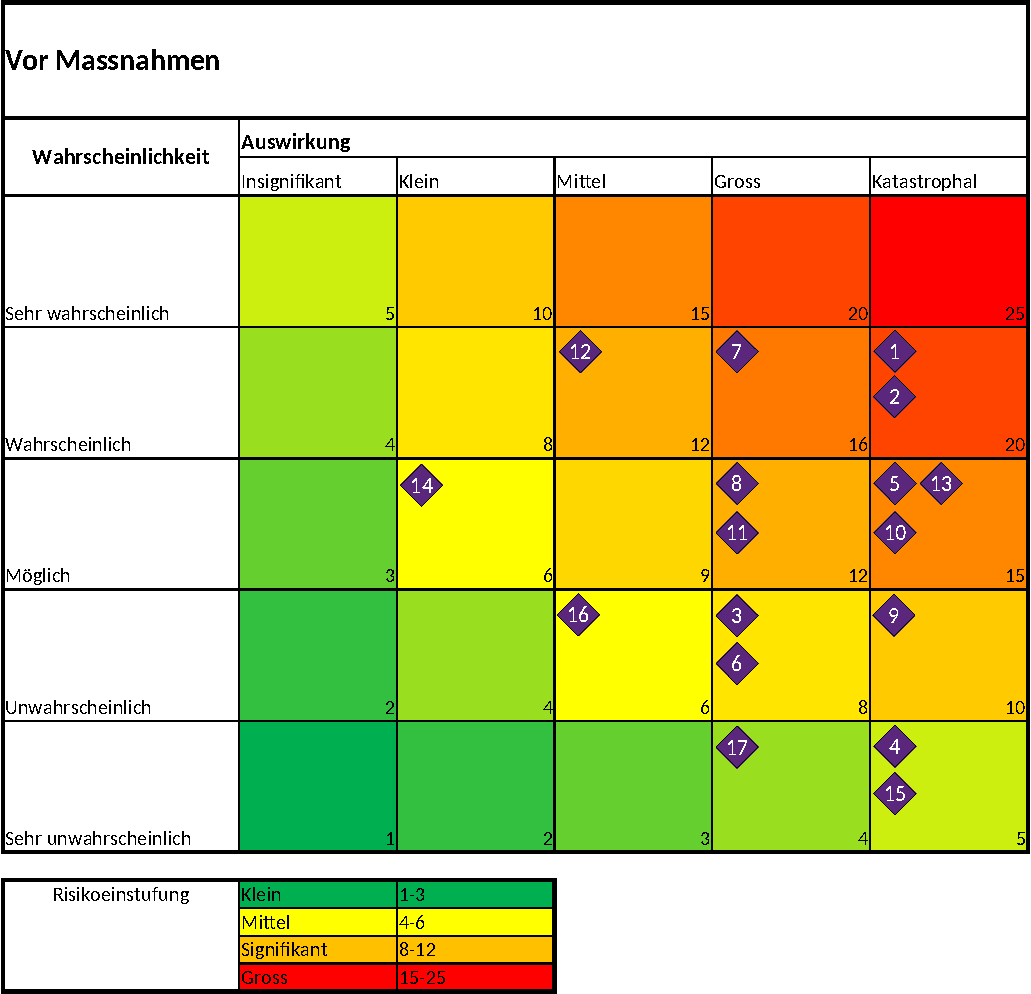
\includegraphics[width=0.99\linewidth]{assets/Risikoanalyse_vor_Massnahmen.pdf}
\caption{vor Massnahmen}
\label{table:risk-before}
\end{subtable}
\begin{subtable}{0.5\textwidth}
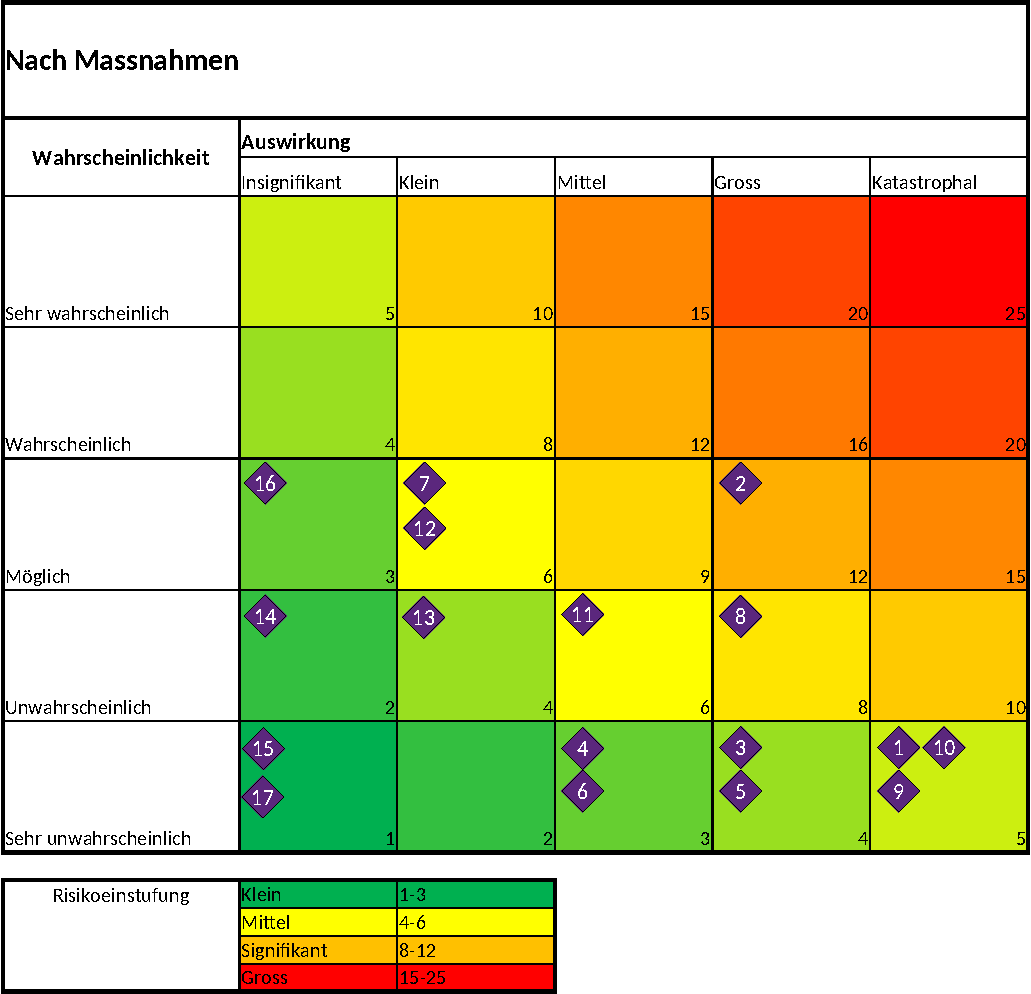
\includegraphics[width=0.99\linewidth]{assets/Risikoanalyse_nach_Massnahmen.pdf}
\caption{nach Massnahmen}
\label{table:risk-after}
\end{subtable}
\caption{Risikoanalyse}
\label{table:risk-table}
\end{table}

Aus der Risikomatrix nach den Massnahmen geht hervor, dass die grössten Risiken, die beim Entwickeln des Roboters berücksichtigt werden müssen, die folgenden drei sind:

\begin{itemize}
    \item Risiko 2: Knoten werden nicht erkannt.
    \item Risiko 7: Ein Objekt wird fehlerhaft gedeutet und falsche Wege werden intern entfernt.
    \item Risiko 12: Der Roboter wählt einen falschen Pfad, weil die Hinderniserkennung fehlerhaft ist.
\end{itemize}

Die folgende Tabelle zeigt alle Risiken detailliert auf.

\begin{table}[H]
\centering
\small
\begin{tabularx}\textwidth{|c | X | X | X | c | c|}
\hline
  \textbf{Nr} & \textbf{Beschreibung} & \textbf{Prävention} & \textbf{Mitigation} & \textbf{V.} & \textbf{N.} \\
  \hline
    1&Hindernisse werden nicht erkannt. &Mit vielen Bildern trainieren.& Distanzsensor erkennt Hindernisse, falls Bilderkennung nicht erkannt hat; Roboter fährt zurück, falls Distanzsensor erkennt.&20&5 \\
  \hline
      2&Knoten werden nicht erkannt. &Viele Bilder in verschiedenen Situationen machen, um zu trainieren.&Linien werden erkannt und Roboter orientiert sich daran.&20& 12\\
  \hline
      3&4 Minuten reichen nicht. &Testdurchfläufe in realistischen Umgebungen.&&8&4 \\
  \hline
      4& 1 Minute reicht nicht zum Aufbau.& Testdurchfläufe und einfaches Interface.&Zufälliges Ziel wird gewählt von SW, falls bei Start keines ausgewählt.&5&3 \\
  \hline
      5&Bodenfugen werden als Linie erkannt. & Testdurchfläufe in realistischen Umgebungen.&Kamera hilft Linien zu erkennen, hilft Roboter gerade zu stellen.&15&4 \\
  \hline
      6& Liniensensor fehlerhaft. &Sichere Implementation mit Tests.& Encoder Motoren.&8&3 \\
  \hline
      7& Ein Objekt wird fehlerhaft gedeutet und falsche Wege werden intern entfernt. &Knoten erkennen und nicht nur Hindernisse.&Roboter ist schnell genug, um Wege auszuprobieren und hat einen Trial \& Error Modus, der dies erlaubt.&16&6 \\
  \hline
      8&Hindernisse werden beim Anheben verschoben. &Robuste Greifmethode wählen und testen.&&12&8 \\
  \hline
      9&Überstrom bei blockierten Motoren. &Endschalter, Stromsensoren.&Abschalten bevor Bauteile beschädigt.&10&5 \\
  \hline
      10&Ungenaue Abfahrtsituation vom Knoten, Fahrzeug fährt von der Linie weg. &Liniensensor als Unterstützung, Kamera prüft Linie& Falls keine Linie mehr erkannt, rückwärts fahren und korrigieren.&15&5 \\
  \hline
      11&Die Kamera liefert unscharfe oder verzerrte unbrauchbare Bilder. &Verwendung von Kameras mit hoher Auflösung.&Falls Bilder unscharf sind, Roboter anhalten und neue Bilder aufnehmen.&12&6 \\
  \hline
      12& Der Roboter wählt einen falschen Pfad, weil die Hinderniserkennung fehlerhaft ist.&Optimierung der Hinderniserkennung.& Falls Fehlzustand auftritt, kann Roboter zu vorherigen Knoten fahren und das vorher gelernte zurücksetzen. Roboter ist schnell.&12& 6\\
  \hline
      13&Ein Softwarefehler führt zu einem Absturz während der Laufzeit, wodurch der Roboter stoppt oder Fehlfunktionen aufweist. &Exception Handling und umfangreiche Tests unter verschiedenen Bedingungen.&Automatischer SW-Neustart, Wiederaufnahme des letzten bekannten Zustands.&15&4 \\
  \hline
\end{tabularx}
\end{table}

\newpage

\begin{table}[H]
\centering
\small
\begin{tabularx}\textwidth{|c | X | X | X | c | c|}
\hline
  \textbf{Nr} & \textbf{Beschreibung} & \textbf{Prävention} & \textbf{Mitigation} & \textbf{V.} & \textbf{N.} \\
  \hline
      14&Ein Software-Update führt zu neuen Fehlern oder ist nicht kompatibel mit der aktuellen Hardware. &Gründliche Tests vor dem Rollout eines Updates.& Durch SW-Versionierung hat man die Möglichkeit, schnell zur vorherigen stabilen Version zurückzukehren.&6&2 \\
  \hline
      15&Akkustand ist zu niedrig bei Start des Laufes. & Anzeige des Akkustandes. Leicht austauschbarer Akku. Akku aufladen.&Ein zweiter Akku, der voll aufgeladen ist.&5& 1\\
  \hline
      16&Personenausfall durch Krankheit oder Unfall. &&Stellvertretungen und virtuelle Kommunikation.&6& 3\\
  \hline
      17&Datenkorruption. &&Regelmässige Backups. Alle Dokumente auf Teams erstellen. Dokumentation in LaTeX auf Overleaf. Durch Cronjob werden jeden Tag die .tex Files auf GitHub gepusht.&4& 1\\
  \hline



\end{tabularx}
\caption{Risiken}
\label{table:risks}
\end{table}





    
    \section{Schlussdiskussion}

In den folgenden Kapiteln wird zusammengefasst, was in \acrshort{pren1} bearbeitet wurde.
Dabei werden die Resultate zusammengefasst mit Ausblick auf \acrshort{pren2}.
Ausserdem werden die Kosten von diesem und nächstem Semester aufgezeigt.
Als letztes werden die gesammelten Erfahrungen bezüglich der Arbeiten und der Zusammenarbeit im Team beschrieben.

\subsection{Erfüllung der Anforderungen}

Im Rahmen von \acrshort{pren1} wurde das Konzept des Roboters als erstes in Teilfunktionen zerlegt, daraus wurde eine Technologierecherche duchgeführt. Aus den Recherchen wurden mithilfe von morphologischen Kasten für die einzelnen Teilbereiche Lösungsvarianten erarbeitet. Diese wurden mit Nutzerwertanalysen bewertet. Die Varianten, die am besten abschlossen, wurden im nächsten Schritt mit Prototyping verfeinert und getestet. Daraus wurde ein Gesamtkonzept erarbeitet und dokumentiert. Ebenfalls wurden 3 physische Prototypen erstellt, die einzelne Teilbereiche des Roboters darstellen. Diese dienen in \acrshort{pren2} dazu, dass damit parallel entwickelt werden kann. Die drei Prototypen sind ein Greifer, ein Kameraturm und ein Fahrwerk.

Das Konzept unseres Roboters hat drei Räder, wovon zwei mit Motoren angetrieben werdem. Diese dienen zur Fortbewegung und zur Lenkung. Die Linienerkennung erfolgt mittels Fototransistoren. Die Hebervorrichtung, die der Roboter braucht, um bewegliche Hindernisse zu beseitigen, wird mit einem Greifer umgesetzt, der zum Klemmen und Anheben einen den selben Servomotor besitzt. Mit einem Ultraschallsensor wird die anzuhebende Barriere erkannt. 
Hindernisse werden mit einer Kamera fotografiert und mit Bilderkennung analysiert. So weiss der Roboter, welche Wege befahrbar sind. Die Navigation wurde in einem Simulator getestet.

Somit wurde das Design für den Roboter erfolgreich erstellt und getestet. Mit diesem Design wird der Roboter in der Lage sein, die Anforderungen, die zu Beginn des Projektes erarbeitet wurden (siehe Kapitel \ref{anforderungliste}), zu erfüllen.

\subsubsection{Ausblick PREN 2}

Aus dem erstellten Design wird nun ein Roboter gebaut. Dabei werden die Einzelteile erstellt und möglichst früh zusammengeführt, um das Zusammenspiel aller Komponenten zu testen.

\textbf{Ausblick Mechanik}

In einem nächsten Schritt in der Anfangsphase von \acrshort{pren2} werden die Erkenntnisse aus den Tests mit den Prototypen aus \acrshort{pren1} ausgewertet. Auf Basis dieser Erkenntnisse wird ein finaler Roboter entwickelt, der alle Teilfunktionen vereint.   

\textbf{Ausblick Steuerung}

Bei den getesteten Hardware Komponenten  muss in einem nächsten Schritt die Software implementiert werden, sodass die Steuerung für das finale Fahrzeug aufgebaut werden kann. Die Schwierigkeit wird dabei sein, die Daten richtig zu verarbeiten wie auch die Kommunikation zwischen Mikrocontroller und der Bilderkennung herzustellen.

\textbf{Ausblick Navigation}

Bezüglich der Navigation bedeutet das, dass nun die Logik des Simulators mit den Prototypen der Bild- und Objekterkennung zusammengefügt werden. Die einzelnen Teile der Objekterkennung werden in einem Workflow zusammengefügt und die Resultate werden in der Simulatorlogik verwendet. Für die Bilderkennung wird ein Model trainiert, dass die Hindernisse und Knoten des Wegenetzes erkennen und auswerten kann. Dieses wird ebenfalls in den Workflow integriert.

Dieser erstellte Workflow wird extensiv getestet und bei Bedarf überarbeitet werden.

\textbf{Risiken}

Die erarbeiteten Risken werden in \acrshort{pren2} weiterhin berücksichtigt. Dabei wird vor allem auf diese Risiken geachtet, die als die drei grössten Risiken erkannt wurden.

\begin{itemize}
    \item Risiko 2: Knoten werden nicht erkannt.
    \item Risiko 7: Ein Objekt wird fehlerhaft gedeutet und falsche Wege werden intern entfernt.
    \item Risiko 12: Der Roboter wählt einen falschen Pfad, weil die Hinderniserkennung fehlerhaft ist.
\end{itemize}

Zusätzlich wächst der Zeitdruck. Die Einzelteile müssen parallel erstellt werden und möglichst früh kombiniert werden, da in diesem Schritt wahrscheinlich noch viele Fehler entdeckt werden, die behoben werden müssen. 

Ausserdem wird ein Studierender aus der Maschinentechnik das Team am Ende von \acrshort{pren1} verlassen und eine neue Person wird in \acrshort{pren2} beitreten. Dabei entsteht das Risiko, dass Wissen verloren geht. Diesem wurde so gut wie möglich entgegen gewirkt, durch regelmässigen Wissensaustausch und Dokumentation von den Arbeiten des Studierenden, der das Team verlässt.

\subsection{Kosten}\label{kosten}

Insgesamt stehen für \acrshort{pren1} und \acrshort{pren2} 500.- zur Verfügung. Im folgenden wird aufgezeigt wie viel davon bereits verwendet wurde und wie viel voraussichtlich noch nächstes Semester benötigt wird.

- Kosten
- angefallene Kosten in PREN1
- Ausblick Gesamtkosten

\begin{table}[H]
\centering
\begin{tabularx}\textwidth{|X | X | X | X |}
\hline
  \textbf{Bezeichnung} & \textbf{Anzahl} & \textbf{Stückpreis} & \textbf{Gesamtkosten} \\
  \hline
    Getriebemotor mit Encoder & 2 &CHF 29.90 & CHF 59.80\\
  \hline
    Raspberry Pi Camera Module 3 & 1 & CHF 29.90& CHF 29.90\\
  \hline
  Raspberry Pi 5 4GB & 1 & CHF 60.90 & CHF X 60.90\\
  
  \hline
    Servomotor aus eigenem Bestand & 1 & CHF 10.00 & CHF 10.00\\
    
  \hline
    PLA-Kunststofffilament & 750g & CHF 15.00 & CHF 15.00\\     

 \hline
    Diverse Schrauben, Muttern und Gewindeeinsätze & X & CHF 10.00 & CHF 10.00\\ 
    
    \hline
   Piezo-Buzzer & 1 & CHF 0.92 & CHF 0.92\\



    \hline
Abstandssensor ToF-based & 1 & CHF 5.71 & CHF 5.71\\

    \hline
Ultraschallsensor & 1 & CHF 5.39 & CHF 5.39\\    

    \hline
\acrshort{i/o} Expander I2C 8-bit & 1 & CHF 1.57 & CHF 1.57\\


\hline
Optical Sensor Development Tools Line Sensor & 2 & CHF 3.00 & CHF 6.00\\


\hline
Pololu QTR-8RC Reflectance Sensor Array & 1 & CHF 8.36 & CHF 8.36\\


\hline
Doppel H-Brücke DC Motor Controller Board in PREN 2& 1 & CHF 8.00 & CHF 8.00\\

\hline
Joy-it SBC-Buck02 Spannungsregler 5V in PREN 2& 2 & CHF 8.15 & CHF 16.30\\

\hline
Diverse Elektronischen Komponenten wie Widerstände und Kondensatoren in PREN 2& X & CHF 10.00 & CHF 10.00\\

\hline
Diverse Litzen und Kabel in PREN 2& X & CHF 10.00 & CHF 10.00\\

\hline
Buzzer in PREN 2& 1 & CHF 6.90 & CHF 6.90\\


  \hline
  \hline
  \textbf{Gesamtkosten} && &CHF 1000\\
  \hline
\end{tabularx}
\caption{Kosten}
\label{table:costs}
\end{table}

\subsection{Lessons Learned}

Wir hatten als Team die Möglichkeit von Grund auf ein Projekt zu planen. Wir haben gelernt eine Aufgabenstellung zu analysieren und mithilfe eines morphologischen Kastens Lösungsvarianten zu finden und die beste davon zu bestimmen. Durch das viele Prototyping haben wir zum einen mehr über die jeweiligen Technologien gelernt und zum anderen haben wir gelernt organisiert unsere Ideen zu testen und aufgrund der Testresultate zu überarbeiten.

\acrshort{pren1} war das erste interdisziplinäre Modul für uns. Dies stellte für uns eine Chance dar.

Wir hatten die Möglichkeit Einblicke in andere Studiengänge zu erhalten. Das heisst, dass wir ein oberflächliches Verständnis für andere Kompetenzen erlangen konnten und ebenfalls unterschiedliche Herangehensweisen beobachten konnten.
Die Herangehensweise, um eine Lösung für ein Problem zu finden, ist bei jeder Person anders. Es konnten klare Unterschiede zwischen den einzelnen Studiengängen beobachtet werden.
Beispielsweise wurde in der Informatik bereits schnell mit dem Entwickeln begonnen, es gab nur eine kurze Designphase, jedoch gab es in der Maschinentechnik grundsätzlich eine längere Designphase, bevor gebaut wurde.

Durch diese unterschiedlichen Herangehensweisen konnten wir voneinander lernen.
Wir wissen nun, was bei interdisziplinären Arbeiten zu erwarten ist und wir haben neue Arten gelernt, wie wir selber in Zukunft vorgehen können.

Bereits ab sechs Teammitgliedern kann es chaotisch werden, vor allem wenn diese recht klar an unterschiedlichen Punkten arbeitet.
Wir haben zu Beginn eine Projektleiterin gewählt, um eine Person zu haben, welche den Überblick über das Gesamtprojekt behält
Dies hat bei der Organisation sehr geholfen. Ebenfalls war es sehr hilfreich, dass wir uns jede Woche getroffen und ausgetauscht haben. Die Kommunikation ist sehr wichtig in Projektarbeiten und dies ist uns gelungen.

Wir sind stolz auf unser finales Design, unsere neu erworbenen Kompetenzen und auf unsere Zusammenarbeit im Team. Während dem letzten Semester haben wir vieles gelernt und wir fühlen uns bereit für \acrshort{pren2}.






    % 

\section{Template}
\subsection{Some subsection}
Lorem ipsum dolor sit amet, officia excepteur ex fugiat reprehenderit enim labore culpa sint ad nisi Lorem pariatur mollit ex esse exercitation amet. Nisi anim cupidatat excepteur officia. Reprehenderit nostrud nostrud ipsum Lorem est aliquip amet voluptate voluptate dolor minim nulla est proident. Nostrud officia pariatur ut officia. Sit irure elit esse ea nulla sunt ex occaecat reprehenderit commodo officia dolor Lorem duis laboris cupidatat officia voluptate. Culpa proident adipisicing id nulla nisi laboris ex in Lorem sunt duis officia eiusmod. Aliqua reprehenderit commodo ex non excepteur duis sunt velit enim. Voluptate laboris sint cupidatat ullamco ut ea consectetur et est culpa et culpa duis.

\subsection{Another subsection: Liste}
How to make a bullet-point list.
\begin{itemize}
    \item First item
    \item Second item
    \item Third item
\end{itemize}

 And another one:
 
\begin{itemize}
    \item First item
    \item Second item
\end{itemize}
\subsection{Third subsection: Nummerierte Liste}
How to make a numbered list:
\begin{enumerate}
    \item First enum
    \item Second enum
    \item Third enum
\end{enumerate}
\subsubsection{Some sub-subsection}
Lorem ipsum dolor sit amet, qui minim labore adipisicing minim sint cillum sint consectetur cupidatat.


\subsection{Some subsection: Bild einfuegen}
Lorem ipsum dolor sit amet, officia excepteur ex fugiat reprehenderit enim labore culpa sint ad nisi Lorem pariatur mollit ex esse exercitation amet. Nisi anim cupidatat excepteur officia. Reprehenderit nostrud nostrud ipsum Lorem est aliquip amet voluptate voluptate dolor minim nulla est proident. Nostrud officia pariatur ut officia. Sit irure elit esse ea nulla sunt ex occaecat reprehenderit commodo officia dolor Lorem duis laboris cupidatat officia voluptate. Culpa proident adipisicing id nulla nisi laboris ex in Lorem sunt duis officia eiusmod. Aliqua reprehenderit commodo ex non excepteur duis sunt velit enim. Voluptate laboris sint cupidatat ullamco ut ea consectetur et est culpa et culpa duis.

\begin{figure}[h]
\centering

\includegraphics[width=\textwidth]{img/HSLU_Logo.png}
\caption{Sample caption}
\label{fig:hslu-logo}
\end{figure}

Here we can reference image \ref{fig:hslu-logo} if a label has been defined when inserting the image. If you do this it will be uniform.

\subsubsection{Some sub-subsection: Tabelle}

This is how you make a table and reference it like this: \ref{table:template}:

\begin{table}[h!]
\centering
\begin{tabular}{ |l| l| l|} % Dimension breite
  \textbf{Column Header 1} & \textbf{Column Header 2} &  \textbf{Column Header 3}\\
  \hline
  
  Row 1, Col1 & Row 1, Col 2 & Row 1, Col 3\\

  Row 2 &Row 2 & Row 2 \\
  
  Row 3 & Row 3 & Row 3 \\
  
  
  Only fill first Col && and the last\\
\end{tabular}
\caption{Table to show how to use tables}
\label{table:template}
\end{table}

\subsection{Subsection: Akronyme und Quellen}

For acronym entries, add them to the "glossary.tex" file and reference them like this: \acrfull{pren1} when you use them for the first time.

When you wanna use the short form do this \acrshort{pren1}.

How to use a source\cite{wikipedia-scrum}.

%%%%%%%%%%%%%%%%%%%%%%%%%%%%%%%%%%%%%%%%%%%%%%%%%%%%%%%%%%%%%%%%%%%%%%%%%%%%%%%%%%%%%%%%%%
%%%%%%%%%%%%%%%%%%%%%%%%%%%%%%%%%%%%%%%%%%%%%%%%%%%%%%%%%%%%%%%%%%%%%%%%%%%%%%%%%%%%%%%%%%
%%%%%%%%%%%%%%%%%%%%%%%%%%%%%%%%%%%%%%%%%%%%%%%%%%%%%%%%%%%%%%%%%%%%%%%%%%%%%%%%%%%%%%%%%%


    % TODO Glossary is ugly
    \newpage
    \addglossary
    \printglossary[]


    % Literaturverzeichnis
  \newpage
  \addcontentsline{toc}
    {section}
    {Literatur}
  \printbibliography[
    heading=subbibliography
  ]

  % Anhang

  \newpage
\section{Anhang}

\subsection{Anforderungsliste}\label{anforderungliste}
Die erste Version der Anforderungsliste ist nachfolgend angehängt.

\begin{table}[H]
\centering
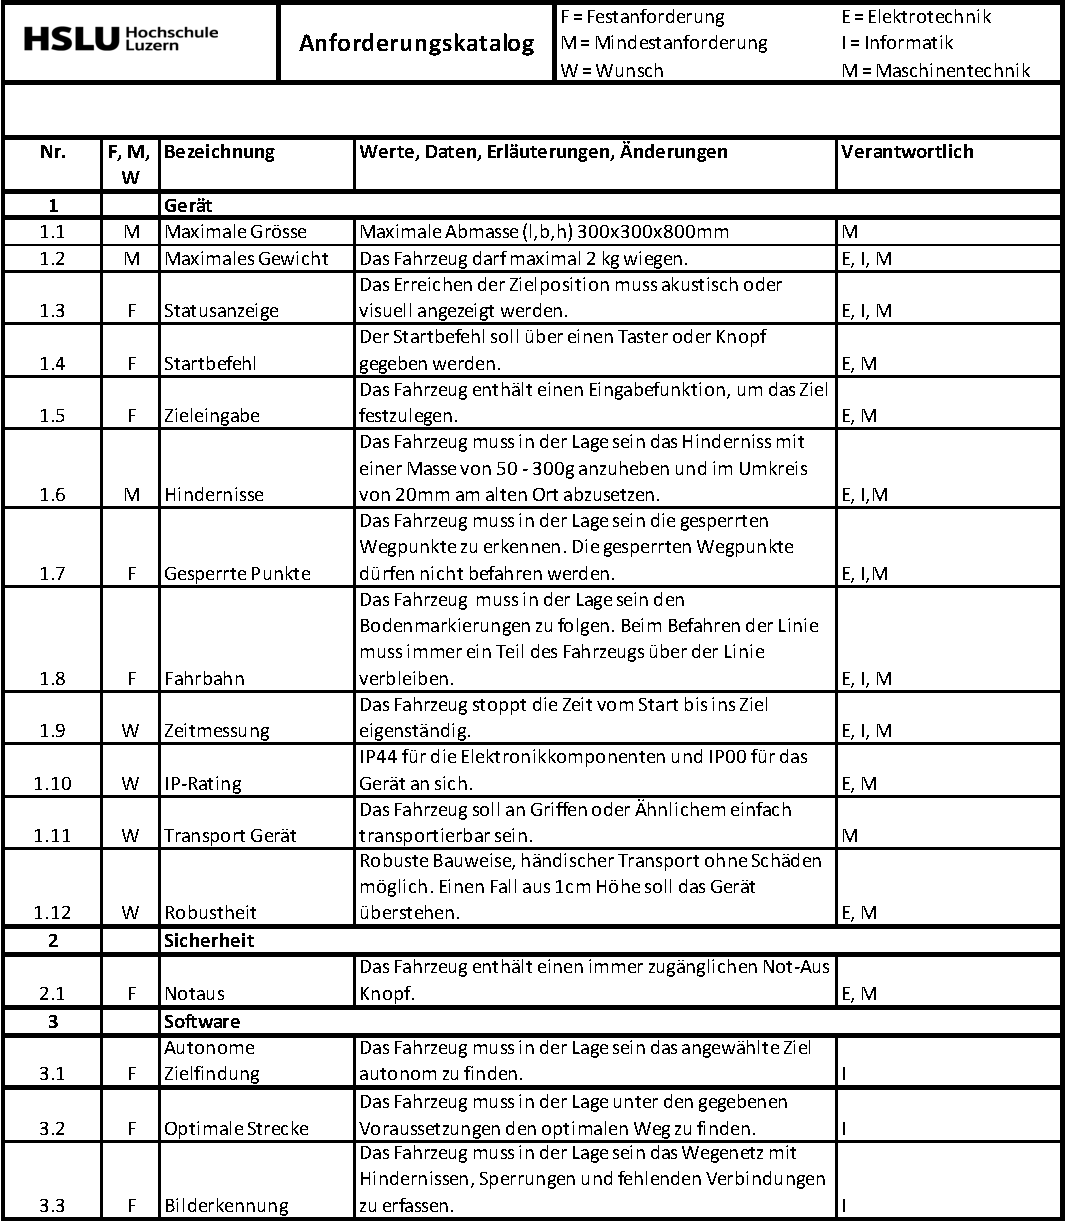
\includegraphics[width=\textwidth]{assets/Anforderungsliste_V1.01_page1.pdf}
\caption{Anforderungsliste Teil 1}
\label{table:anforderungsliste_page1}
\end{table}
\newpage

\begin{table}[H]
\centering
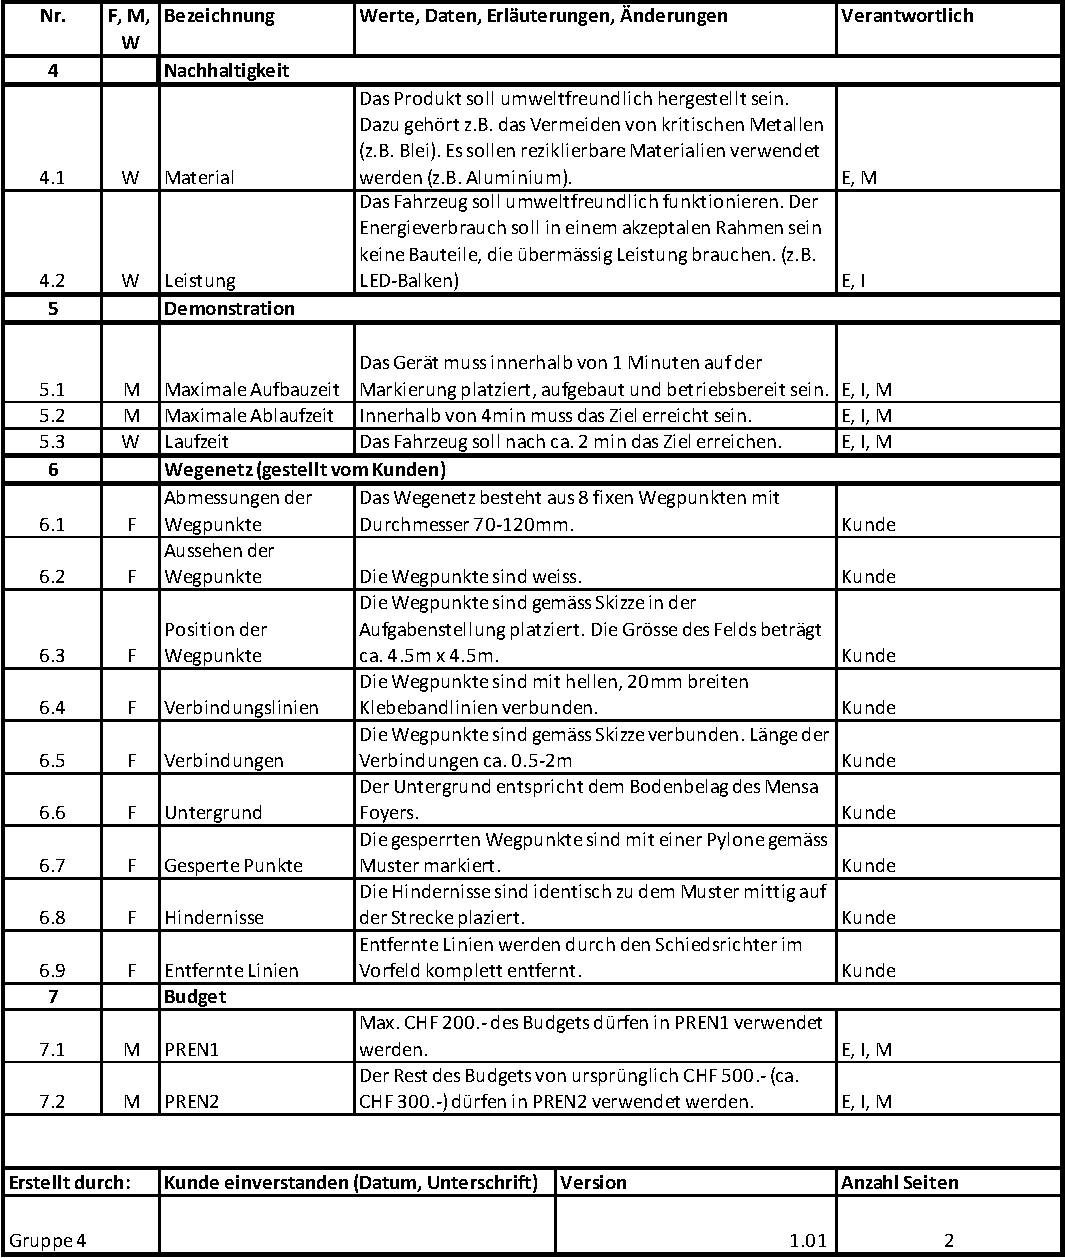
\includegraphics[width=\textwidth]{assets/Anforderungsliste_V1.01_page2.pdf}
\caption{Anforderungsliste Teil 2}
\label{table:anforderungsliste_page2}
\end{table}
\newpage

\begin{landscape}
\subsection{Kommunikationsplan}\label{kommunikationsplan}
Die Kommunikationskanäle sind folgendermassen definiert:

\begin{table}[H]
\centering
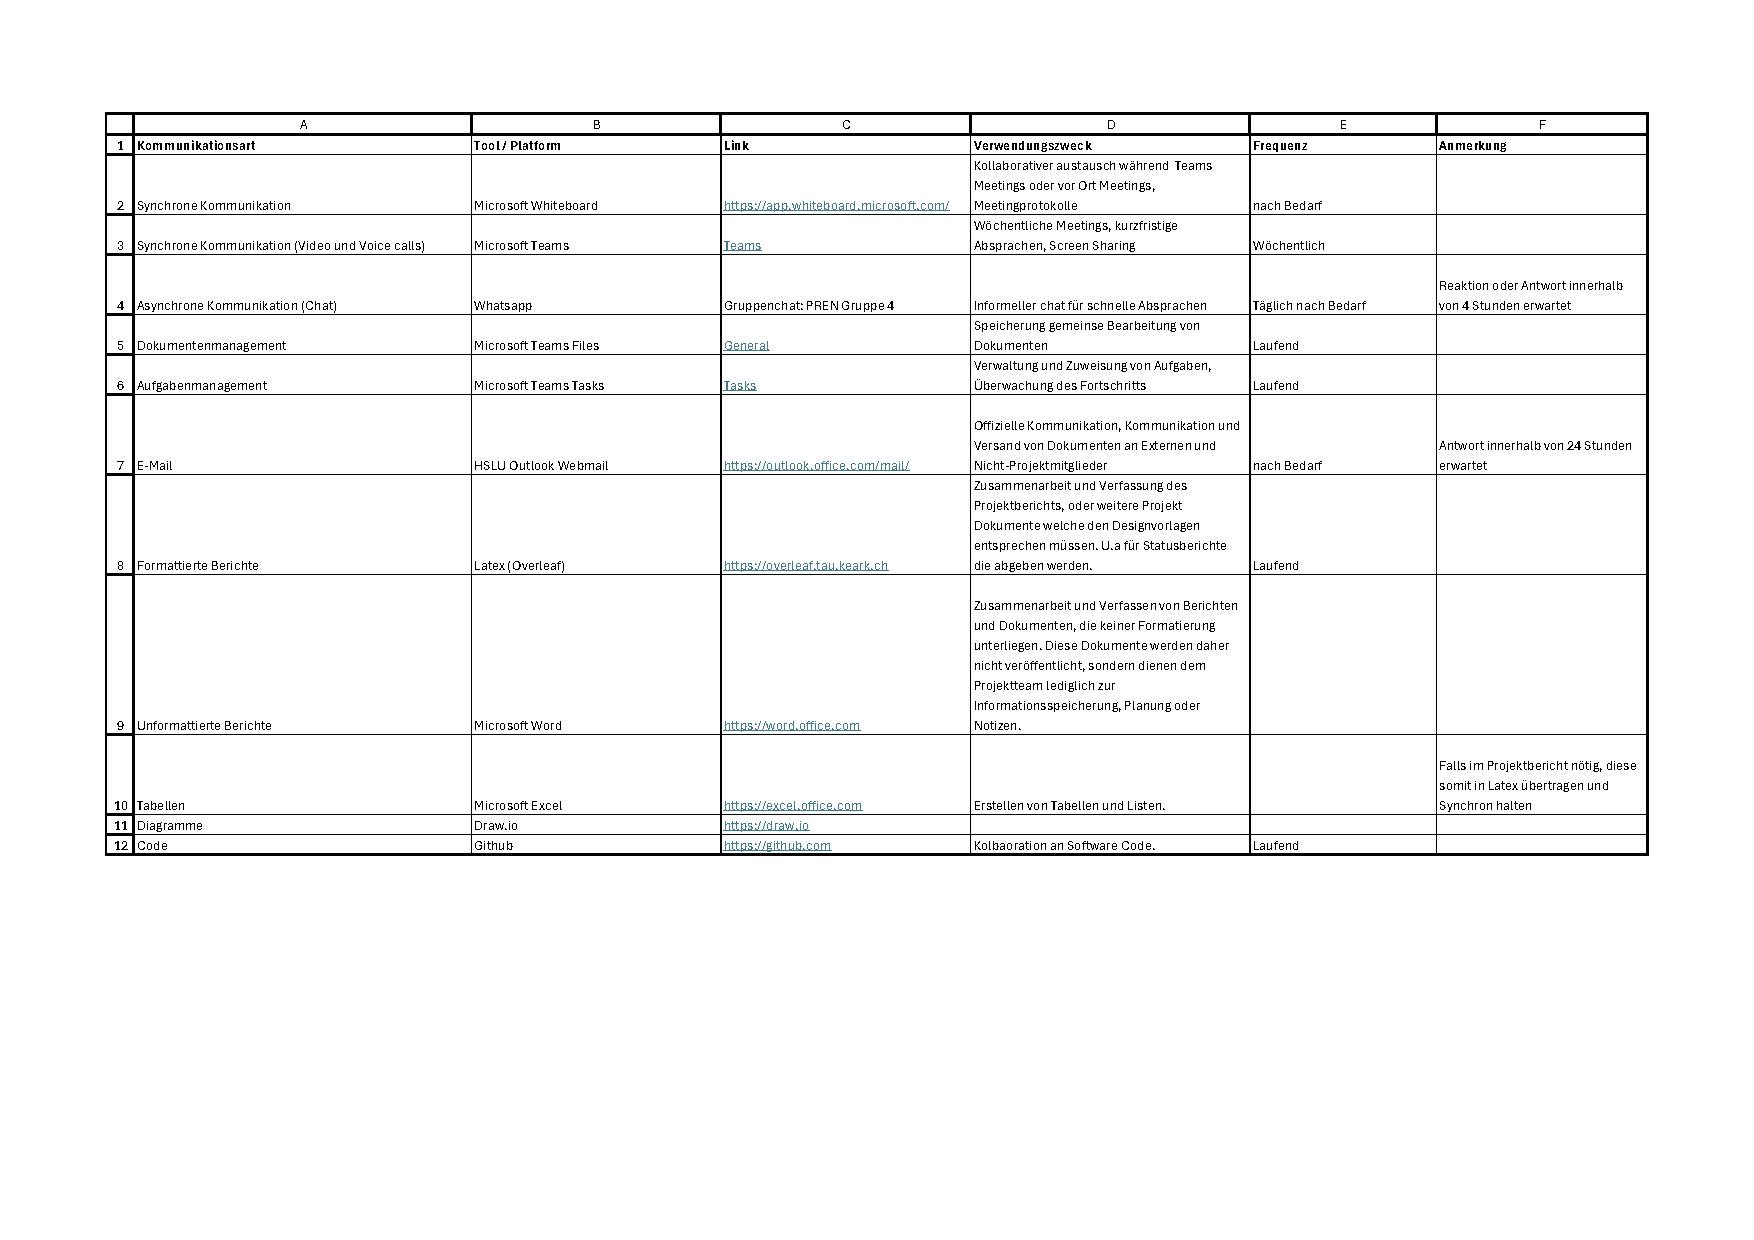
\includegraphics[width=240mm]{assets/Kommunikationschnittstellen.pdf}
\caption{Kommunikationsplan}
\label{table:communications-plan}
\end{table}
\end{landscape}

%%%%%%%%%%%%%%%%%% Technologierecherche %%%%%%%%%%%%%%%%%%%%

\subfile{parts/a-technologierecherchen}


%%%%%%%%%%%%%%%%%%%%%%%%%%%%%%%%%%%%%%%%%%%%%
%%%%%%% Entfernt, weil bereits in Doc   %%%%%
%%%%%%%%%%%%%%%%%%%%%%%%%%%%%%%%%%%%%%%%%%%%%
%\subsection{Morphologischer Kasten}\label{Morphologischer Kasten}
%Nachfolgend die Morphologischen Kästen, unterteilt in die jeweiligen Studiengänge, Elektrotechnik, Informatik und Maschinentechnik. %Jeder Kasten hat 3 Varianten eingezeichnet. Variante A: Gelb, Variante B: Rot, Variante C: Grün.
%
%\begin{table}[H]
%\centering
%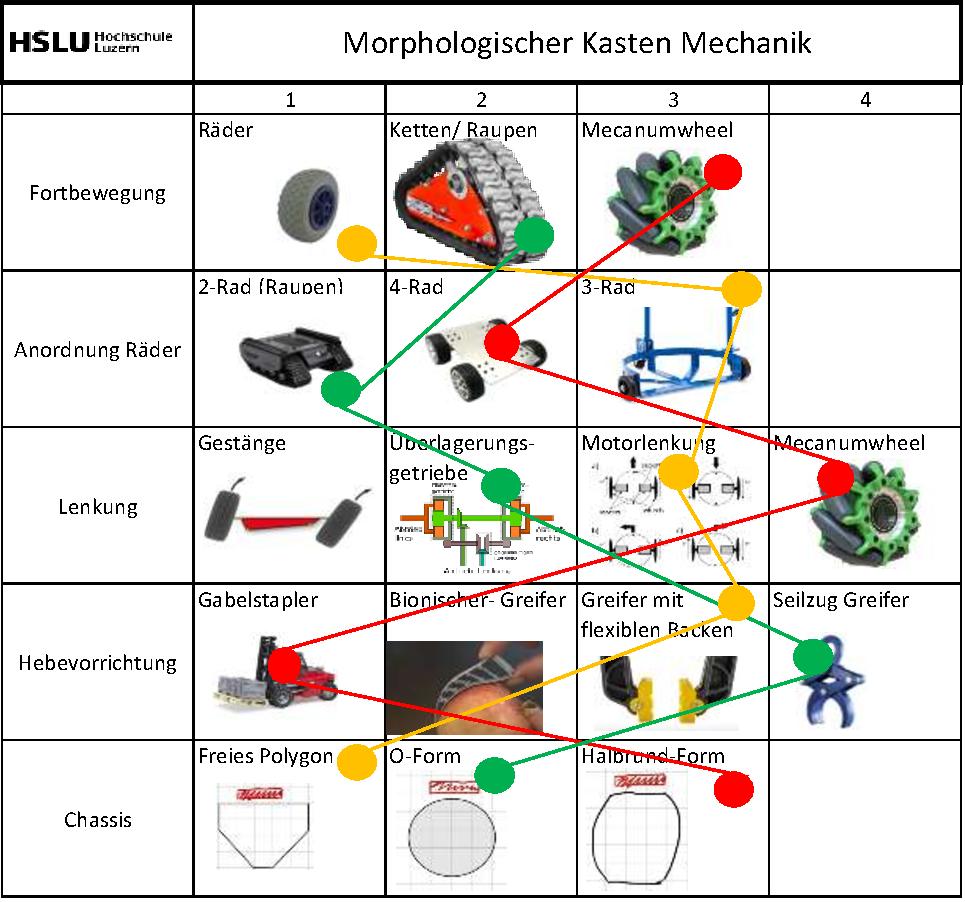
\includegraphics[width=\textwidth]{assets/MK_Maschinentechnik.pdf}
%\caption{Morphologischer Kasten: Maschinentechnik}
%\label{table:MK-Maschinentechnik}
%\end{table}
%\newpage
%\begin{table}[H]
%\centering
%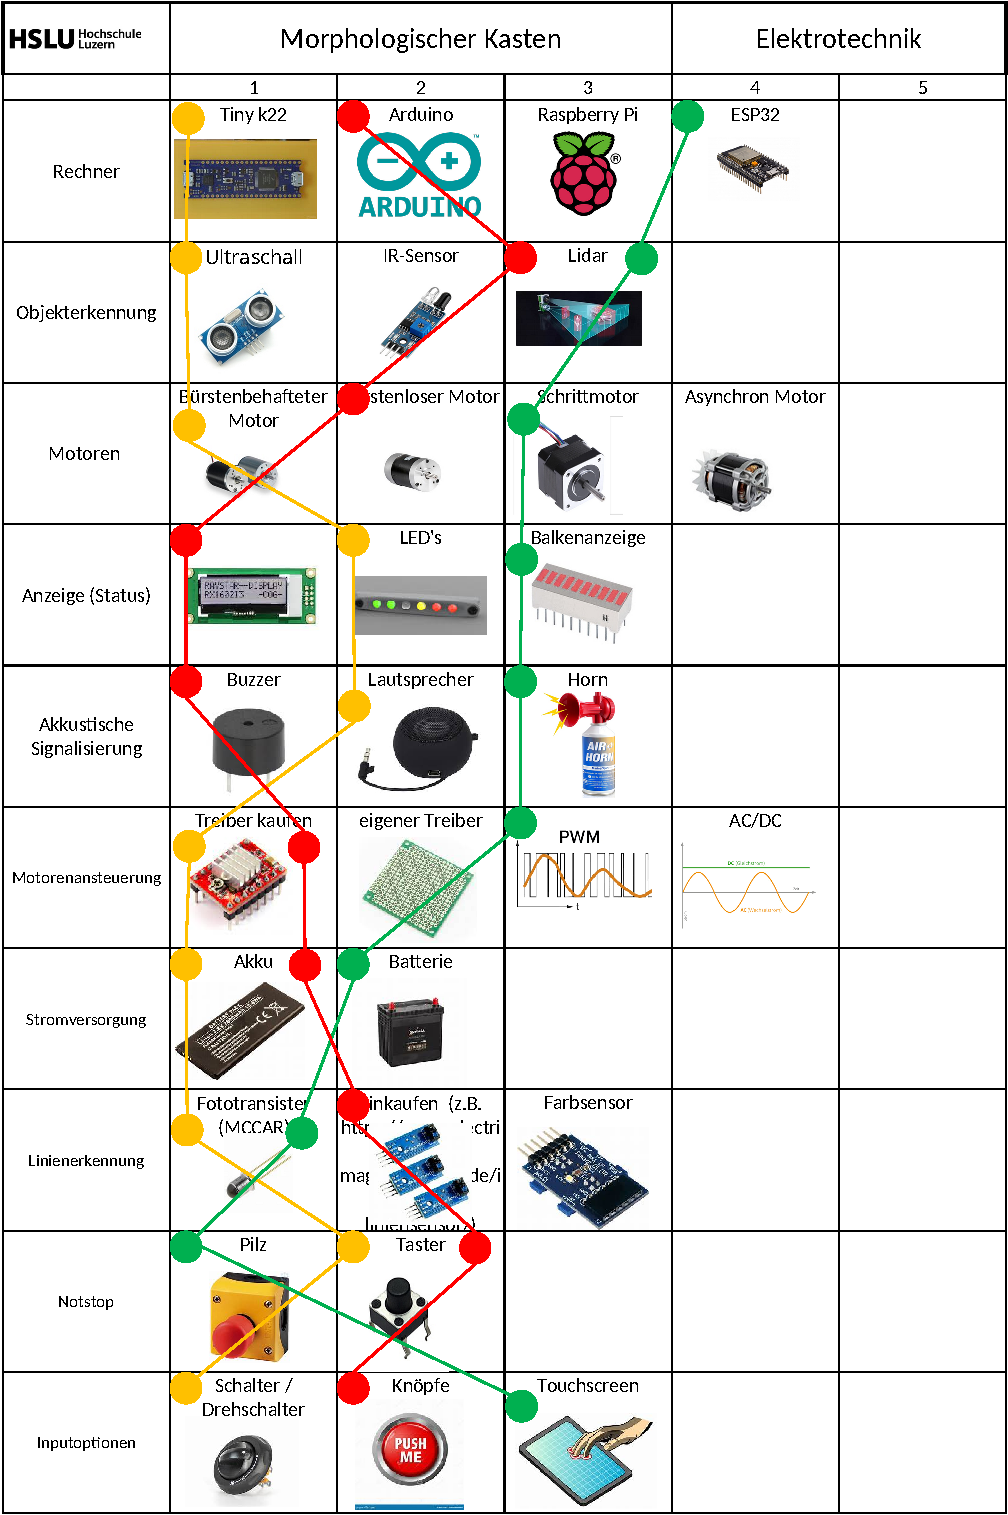
\includegraphics[height=\textheight-1cm]{assets/MK_Elektrotechnik.pdf}
%\caption{Morphologischer Kasten: Elektrotechnik}
%\label{table:MK-Elektrotechnik}
%\end{table}
%\newpage
%\begin{table}[H]
%\centering
%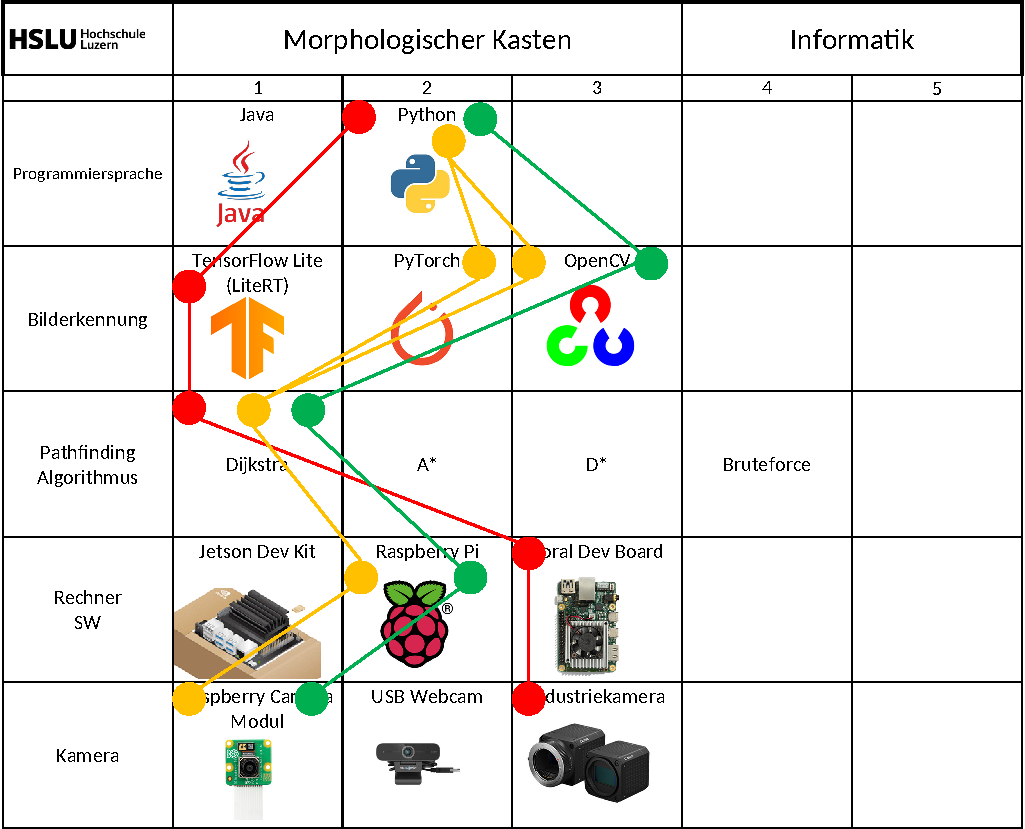
\includegraphics[width=\textwidth]{assets/MK_Informatik.pdf}
%\caption{Morphologischer Kasten: Informatik}
%\label{table:MK-Informatik}
%\end{table}
%\newpage
%\begin{table}[H]
%\centering
%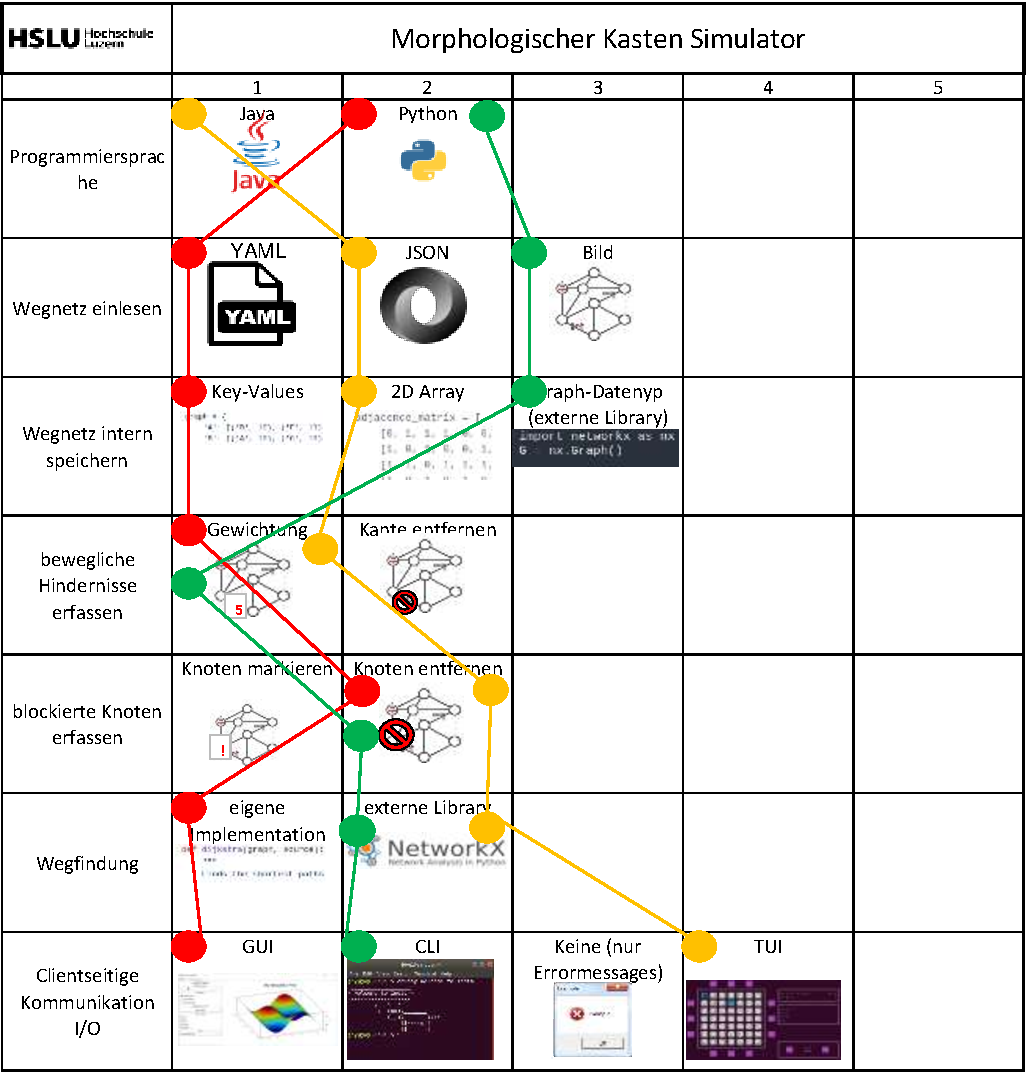
\includegraphics[width=\textwidth]{assets/MK_Simulator.pdf}
%\caption{Morphologischer Kasten: Simulator}
%\label{table:MK-Simulator}
%\end{table}
%\newpage


%%% THIS IS USELESS %%%%%%%%%%%%

% \subsection{Originale Aufgabenstellung}\label{aufgabenstellung}

% Nachfolgend ist die originale Aufgabenstellung angehängt.

% 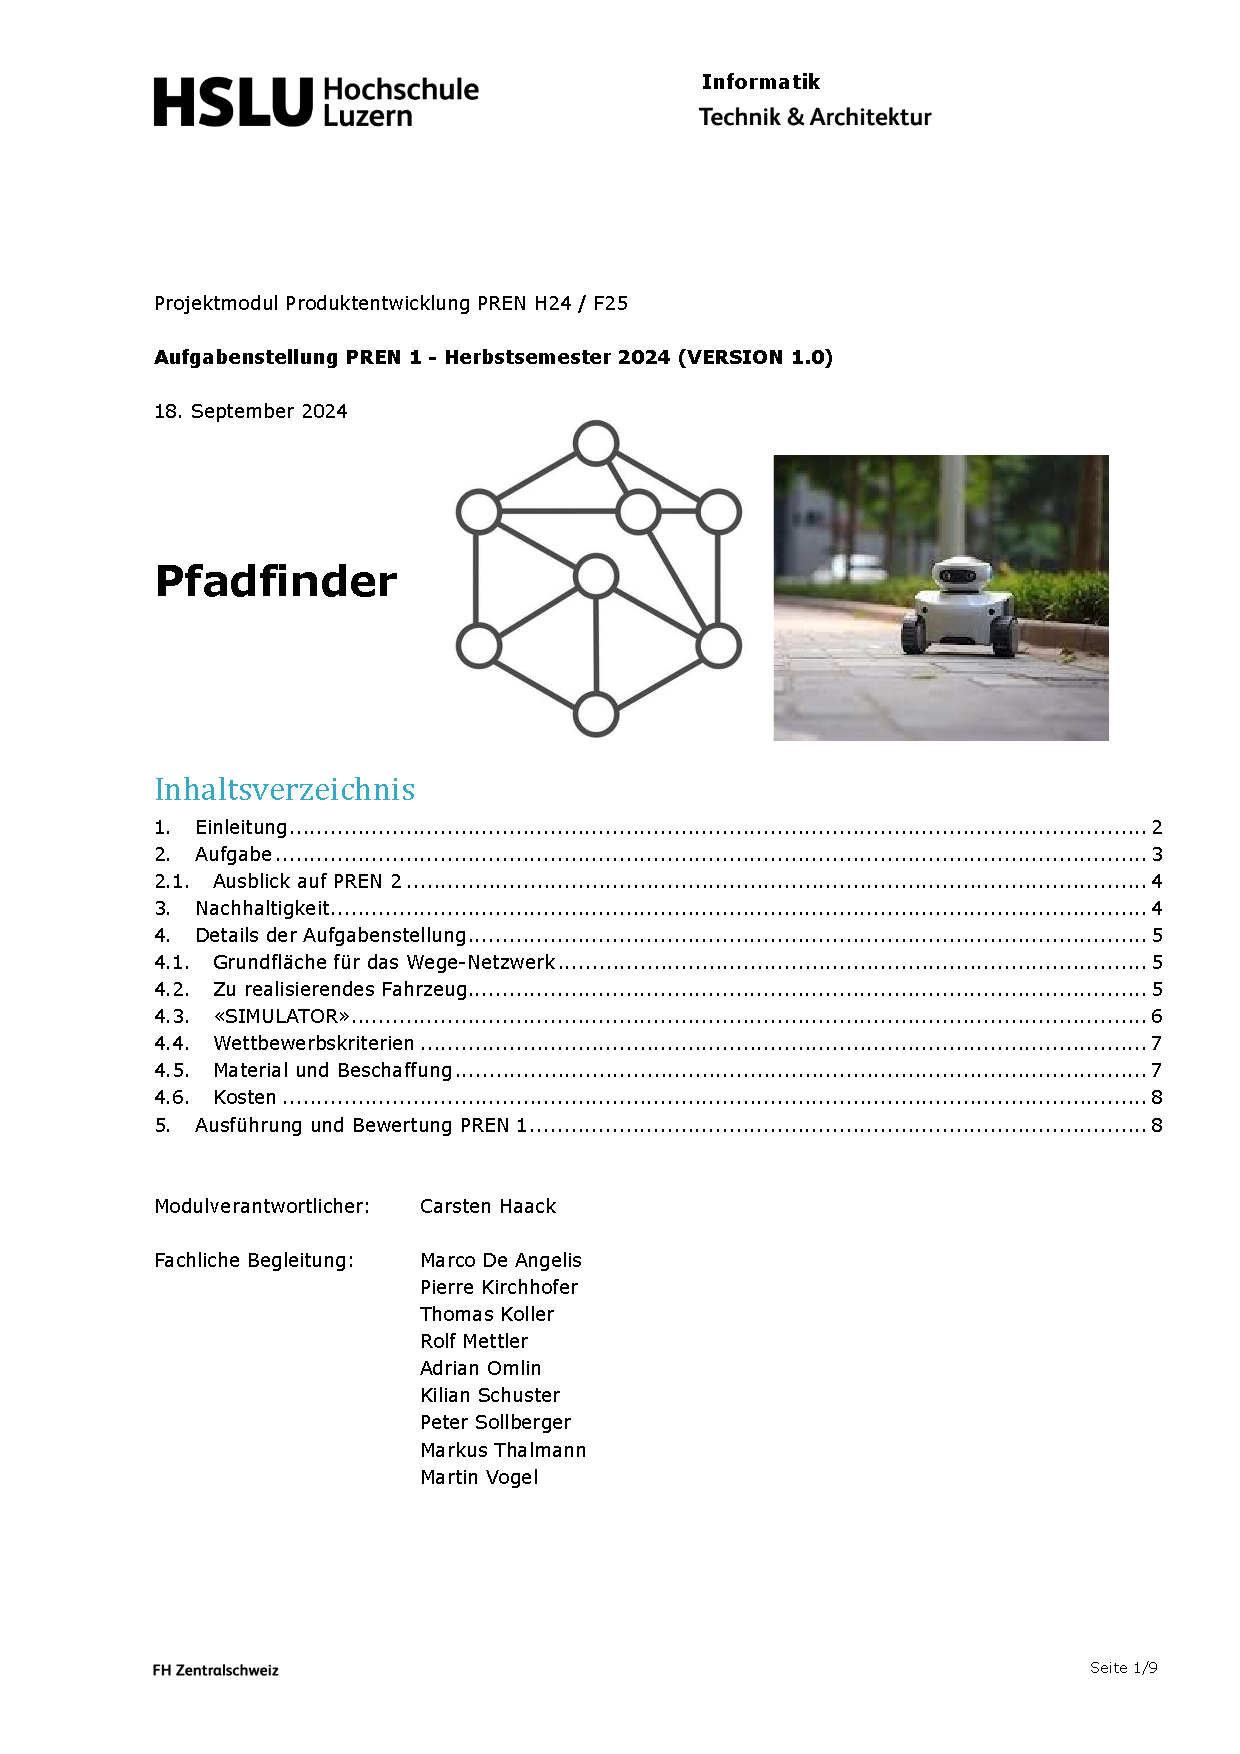
\includepdf[pages=-]{assets/AufgabenstellungPREN1HS24.pdf}



\end{document}